%----------------------------------------------------------------------------------------
%	PACKAGES AND OTHER DOCUMENT CONFIGURATIONS
%----------------------------------------------------------------------------------------

\documentclass[11pt, a4paper, twoside]{Thesis} % Paper size, default font size and one-sided paper

\graphicspath{{./Pictures/}} % Specifies the directory where pictures are stored

%\usepackage[square, numbers, comma, sort&compress]{natbib} % Use the natbib reference package - read up on this to edit the reference style; if you want text (e.g. Smith et al., 2012) for the in-text references (instead of numbers), remove 'numbers' 
\usepackage[natbib=true, maxbibnames=99, maxcitenames=2, giveninits=true, sorting=none]{biblatex}

\hypersetup{urlcolor=black, colorlinks=true} % Colors hyperlinks in blue - change to black if annoying
\title{\ttitle} % Defines the thesis title - don't touch this

\usepackage{tikz}
\usepackage{setspace}

\definecolor{OrangeGSSI}{RGB}{237,113,45}
\definecolor{blue}{RGB}{25,25,112}

%----------------------------------------------------------------------------------------
%	DOCUMENT VARIABLES
%	Fill in the lines below to update the thesis template
%	If you wish to cite each of the variables defined below, look at the
%	section above for the citation command e.g. \examiner{} below is
%	defined as \examname above so you cite it as \examname
%----------------------------------------------------------------------------------------

\title{Orchestration Strategies for Regression Testing of Evolving Software Systems}

\thesistitle{Orchestration Strategies for Regression Testing of Evolving Software Systems} % Your thesis title - this is used in the title and abstract
%-------------------------------------------------  
\supervisor{Prof. Antonia \textsc{Bertolino}} % You supervisor's name - this is used in the title page
%-------------------------------------------------   
\examiner{Dr. Ludovico  \textsc{Iovino}} % Your examiner's name - this is not currently used anywhere in the template, cite it with \examname if you want it
%-------------------------------------------------   
\degree{Doctor of Philosophy} % Your degree name - this is currently used in the title page and abstract
%-------------------------------------------------   
\authors{Renan Domingos\\ \textsc{Merlin Greca}} % Your name - this is used in the title page and abstract
%-------------------------------------------------

%----------------------------------------------------------------------------------------
%	TYPESETTING
%----------------------------------------------------------------------------------------
\usepackage{pifont}
\usepackage{colortbl}
\usepackage{flushend}
\usepackage[normalem]{ulem} % for \sout
\usepackage{multicol}
\usepackage[most]{tcolorbox}
\usepackage[nameinlink]{cleveref}
\usepackage{algorithm}
\usepackage{algorithmicx}
\usepackage[noend]{algpseudocode}
%\usepackage[english]{babel}
\usepackage{hyphenat}
%\usepackage[resetlabels,labeled]{multibib}
\usepackage{multirow}
%\usepackage{bibentry}
%\nobibliography*
%\usepackage[left=1.4cm, right=1cm, top=0.6cm, bottom=0.8cm, paper=a4paper]{geometry}

%\usepackage[left=1cm,right=2cm,vmargin=2.5cm,footnotesep=0.5cm]{geometry}
%
%\setmarginsrb  { 1.4in}  % left margin
%                        { 0.6in}  % top margin
%                        { 1.0in}  % right margin
%                        { 0.8in}  % bottom margin
%                        {  20pt}  % head height
%                        {0.25in}  % head sep
%                        {   9pt}  % foot height
%                        { 0.3in}  % foot sep

%\hyphenation{non-de-ter-mi-nis-ti-cal-ly}

\newcommand{\ugh}[1]{\textcolor{red}{\uwave{#1}}} % please rephrase
\newcommand{\ins}[1]{\textcolor{blue}{\uline{#1}}} % please insert
\newcommand{\del}[1]{\textcolor{red}{\sout{#1}}} % please delete
\newcommand{\chg}[2]{\textcolor{red}{\sout{#1}}{\ra}\textcolor{blue}{\uline{#2}}} % please change

\renewcommand{\ttdefault}{cmr}

%% Abbreviation commands
\newcommand{\tcp}{TCP\xspace}
\newcommand{\tcs}{TCS\xspace}
\newcommand{\tsr}{TSR\xspace}
\newcommand{\tsa}{TSA\xspace}
\newcommand{\rt}{RT\xspace}
\newcommand{\rea}{IR\&A\xspace}
\newcommand{\sut}{SUT\xspace}
\newcommand{\slr}{SLR\xspace}

\newcommand{\ek}{Ekstazi\xspace}
\newcommand{\ekr}{Ekstazi\xspace}
\newcommand{\rnd}{Random\xspace}
\newcommand{\fs}{FAST\xspace}
\newcommand{\fz}{{Fastazi}\xspace}
\newcommand{\fzs}{\fz-S\xspace}
\newcommand{\fzp}{\fz-P\xspace}
\newcommand{\dfj}{Defects4J\xspace}

\newcommand{\apfd}{APFD\xspace}
\newcommand{\ttff}{TTFF\xspace}
\newcommand{\pttff}{TTFF\xspace}

\newcommand{\rotatedheader}[2] {
	\rotatebox[origin=c]{90}{\textbf{{\color{#1} #2}}}
}

\newcommand{\quoter}[2]{``\textit{#1}'' (#2)}
\newcommand{\quotes}[1]{``\textit{#1}''}

\newcommand{\assignedto}[1]{\textcolor{red}{\ding{46}~{\sf Assigned to:}~#1}\\}
\newcommand{\todo}[1]{\textcolor{blue}{\ding{46}{\sf}~#1}}
\newcommand{\sugg}[1]{\textcolor{orange}{#1}}

\newcommand{\anto}[1]{[[\textbf{Anto:}~{\color{olive}#1}]]}
\newcommand{\breno}[1]{[[\textbf{Breno:}~{\color{teal}#1}]]}
\newcommand{\renan}[1]{[[\textbf{Renan:}~{\color{brown}#1}]]}


\definecolor{bronze}{HTML}{666211}
\definecolor{cyprus}{HTML}{006666}
\definecolor{derby}{HTML}{664422}
\definecolor{diesel}{HTML}{660122}
\definecolor{verdun}{HTML}{366600}
\definecolor{midnight}{HTML}{002766}
\definecolor{bossanova}{HTML}{642B66}

% Circles
\usepackage{tikz}
\newcommand*\emptycirc[1][1ex]{%
	\begin{tikzpicture}
		\draw (0,0) circle (#1);
	\end{tikzpicture}} 
\newcommand*\halfcirc[1][1ex]{%
  \begin{tikzpicture}
  \draw[fill] (0,0)-- (90:#1) arc (90:270:#1) -- cycle ;
  \draw (0,0) circle (#1);
  \end{tikzpicture}}
\newcommand*\fullcirc[1][1ex]{%
  \begin{tikzpicture}
	\draw[fill] (0,0) circle (#1);  	
  \end{tikzpicture}} 
  
%\geometry{%
%    paper = a4paper,%
%    top = 0.6in,%
%    left = 1.4in,%
%    right = 1.0 in, %
%    bottom = 0.8in,%         <---- Changing this has no effect
%    headsep = 0.25in%
%}

  
% Defining bibliographies
%\newcites{P}{Papers produced during the development of this thesis}
%\newcites{C}{Conferences related to this thesis}
%\newcites{S}{Papers identified in the Systematic Literature Review}
%\newcites{Bibliography}{Bibliography}

\defbibheading{P}{}
\defbibheading{S}{Papers identified in the Systematic Literature Review}
\defbibheading{R}{Bibliography}

\addbibresource[label=P]{production.bib}
\addbibresource[label=S]{slr.bib}
\bibliography{bibliography.bib, secondaries.bib}


\newcommand{\numpapers}{79\xspace}
\defcitealias{srikanth_requirements_2016}{S1}
\defcitealias{noor_similarity-based_2016}{S2}
\defcitealias{schwartz_cost-effective_2016}{S3}
\defcitealias{hirzel_graph-walk-based_2016}{S4}
\defcitealias{lu_how_2016}{S5}
\defcitealias{vost_trace-based_2016}{S6}
\defcitealias{wang_enhancing_2016}{S7}
\defcitealias{srikanth_test_2016}{S8}
\defcitealias{blondeau_test_2017}{S9}
\defcitealias{pradhan_search-based_2016}{S10}
\defcitealias{buchgeher_improving_2016}{S11}
\defcitealias{tahvili_dynamic_2016}{S12}
\defcitealias{oqvist_extraction-based_2016}{S13}
\defcitealias{magalhaes_automatic_2016}{S14}
\defcitealias{aman_application_2016}{S15}
\defcitealias{busjaeger_learning_2016}{S16}
\defcitealias{yoshida_fsx_2016}{S17}
\defcitealias{tahvili_cost-benefit_2016}{S18}
\defcitealias{ramler_tool_2017}{S19}
\defcitealias{strandberg_experience_2016}{S20}
\defcitealias{marijan_effect_2016}{S21}
\defcitealias{gotlieb_using_2017}{S22}
\defcitealias{chi_multi-level_2017}{S23}
\defcitealias{bach_coverage-based_2017}{S24}
\defcitealias{spieker_reinforcement_2017}{S25}
\defcitealias{vasic_file-level_2017}{S26}
\defcitealias{celik_regression_2017}{S27}
\defcitealias{ouriques_test_2018}{S28}
\defcitealias{kwon_cost-effective_2017}{S29}
\defcitealias{garousi_multi-objective_2018}{S30}
\defcitealias{shi_evaluating_2018}{S31}
\defcitealias{haghighatkhah_test_2018}{S32}
\defcitealias{zhang_hybrid_2018}{S33}
\defcitealias{miranda_fast_2018}{S34}
\defcitealias{yilmaz_case_2018}{S35}
\defcitealias{chen_optimizing_2018}{S36}
\defcitealias{celik_regression_2018}{S37}
\defcitealias{zhu_test_2018}{S38}
\defcitealias{azizi_retest_2018}{S39}
\defcitealias{guo_decomposing_2019}{S40}
\defcitealias{zhong_testsage:_2019}{S41}
\defcitealias{fu_resurgence_2019}{S42}
\defcitealias{eda_efficient_2019}{S43}
\defcitealias{goyal_test_2019}{S44}
\defcitealias{yu_terminator_2019}{S45}
\defcitealias{correia_motsd_2019}{S46}
\defcitealias{machalica_predictive_2018}{S47}
\defcitealias{najafi_improving_2019}{S48}
\defcitealias{leong_assessing_2019}{S49}
\defcitealias{cruciani_scalable_2019}{S50}
\defcitealias{philip_fastlane:_2019}{S51}
\defcitealias{magalhaes_hsp_2020}{S52}
\defcitealias{wu_time_2019}{S53}
\defcitealias{land_industrial_2019}{S54}
\defcitealias{noemmer_evaluation_2020}{S55}
\defcitealias{lubke_selecting_2020}{S56}
\defcitealias{yackley_simultaneous_2019}{S57}
\defcitealias{shi_understanding_2019}{S58}
\defcitealias{lima_multi-armed_2022}{S59}
\defcitealias{zhou_beating_2020}{S60}
\defcitealias{peng_empirically_2020}{S61}
\defcitealias{bertolino_learning--rank_2020}{S62}
\defcitealias{chen_multi-objective_2021}{S63}
\defcitealias{zarges_artificial_2021}{S64}
\defcitealias{bagherzadeh_reinforcement_2022}{S65}
\defcitealias{elsner_empirically_2021}{S66}
\defcitealias{pan_dynamic_2020}{S67}
\defcitealias{mehta_data-driven_2021}{S68}
\defcitealias{xu_requirement-based_2021}{S69}
\defcitealias{zhou_parallel_2022}{S70}
\defcitealias{sharif_deeporder_2021}{S71}
\defcitealias{li_aga_2021}{S72}
\defcitealias{chen_context-aware_2021}{S73}
\defcitealias{zhang_comparing_2022}{S74}
\defcitealias{abdelkarim_tcp-net_2022}{S75}
\defcitealias{cingil_black-box_2022}{S76}
\defcitealias{yaraghi_scalable_2022}{S77}
\defcitealias{omri_learning_2022}{S78}
\defcitealias{greca_comparing_2022}{S79}
  

%----------------------------------------------------------------------------------------
%	End of TYPESETTING
%----------------------------------------------------------------------------------------

\begin{document}

\frontmatter % Use roman page numbering style (i, ii, iii, iv...) for the pre-content pages

\setstretch{1.3} % Line spacing of 1.3

% Define the page headers using the FancyHdr package and set up for one-sided printing
\fancyhead{} % Clears all page headers and footers
\rhead{\thepage} % Sets the right side header to show the page number
\lhead{} % Clears the left side page header

% \pagestyle{fancy} % Finally, use the "fancy" page style to implement the FancyHdr headers
\newcommand{\HRule}{\rule{\linewidth}{0.5mm}} % New command to make the lines in the title page



% PDF meta-data
\hypersetup{pdftitle={\ttitle}}
\hypersetup{pdfsubject=\subjectname}
\hypersetup{pdfauthor=\authornames}
\hypersetup{pdfkeywords=\keywordnames}

%----------------------------------------------------------------------------------------
%	TITLE PAGE
%----------------------------------------------------------------------------------------

%\newgeometry{left=1in}

\begin{titlepage}
\begin{center}


\includegraphics[width=0.4\textwidth]{./figures/logo_GSSI}~\\[1cm]
\textsc{\Large Doctoral Thesis}\\[0.5cm] % Thesis type

\HRule \\[0.1cm] % Horizontal line
{\huge \bfseries  Orchestration Strategies for Regression\\[0.3cm] Testing of Evolving Software Systems }\\[0.3cm] % Thesis title
\HRule \\[0.9cm] % Horizontal line

{\Large \textsc{PhD Program in Computer Science: 34th cycle}}\\[2cm]

\begin{minipage}{0.4\textwidth}
\begin{flushleft} \large
\emph{Author:}\\
\bigskip \authornames \\
\href{mailto:renan.greca@gssi.it}{renan.greca@gssi.it}
%\href{http://www.johnsmith.com}{\authornames} % Author name - remove the \href bracket to remove the link
\end{flushleft}
\end{minipage}
\begin{minipage}{0.5\textwidth}
\begin{flushright} \large
\emph{Supervisors:} \\
%\href{http://www.jamessmith.com}{\supname} % Supervisor name - remove the \href bracket to remove the link  
\bigskip \supname \\
\href{mailto:antonia.bertolino@isti.cnr.it}{antonia.bertolino@isti.cnr.it} \\
Prof. Breno \textsc{Miranda}\\
\href{mailto:bafm@cin.ufpe.br}{bafm@cin.ufpe.br} \\
\bigskip \bigskip
\emph{Internal advisor:} \\
\bigskip \examname \\
\href{mailto:ludovico.iovino@gssi.it}{ludovico.iovino@gssi.it}
\end{flushright}
\end{minipage}\\[2.0cm]
 
%\large \textit{A thesis submitted in fulfilment of the requirements\\ for the degree of \degreename}\\[0.3cm] % University requirement text
%\textit{in the}\\[0.4cm]
%\groupname\\\deptname\\[2cm] % Research group name and department name


{\large \today}\\[2.2cm] % Date

\univname \\
\addressnames
%\includegraphics{Logo} % University/department logo - uncomment to place it
 
\vfill
\end{center}

\end{titlepage}

\cleardoublepage

%\restoregeometry

%----------------------------------------------------------------------------------------
%	DECLARATION PAGE
%	Your institution may give you a different text to place here
%----------------------------------------------------------------------------------------

%\Declaration{
%
%\addtocontents{toc}{\vspace{1em}} % Add a gap in the Contents, for aesthetics
%
%I, \authornames, declare that this thesis titled, '\ttitle' and the work presented in it are my own. I confirm that:
%
%\begin{itemize} 
%\item[\tiny{$\blacksquare$}] This work was done wholly or mainly while in candidature for a research degree at this University.
%\item[\tiny{$\blacksquare$}] Where any part of this thesis has previously been submitted for a degree or any other qualification at this University or any other institution, this has been clearly stated.
%\item[\tiny{$\blacksquare$}] Where I have consulted the published work of others, this is always clearly attributed.
%\item[\tiny{$\blacksquare$}] Where I have quoted from the work of others, the source is always given. With the exception of such quotations, this thesis is entirely my own work.
%\item[\tiny{$\blacksquare$}] I have acknowledged all main sources of help.
%\item[\tiny{$\blacksquare$}] Where the thesis is based on work done by myself jointly with others, I have made clear exactly what was done by others and what I have contributed myself.\\
%\end{itemize}
% 
%Signed:\\
%\rule[1em]{25em}{0.5pt} % This prints a line for the signature
% 
%Date:\\
%\rule[1em]{25em}{0.5pt} % This prints a line to write the date
%}
%
%\clearpage % Start a new page

%----------------------------------------------------------------------------------------
%	QUOTATION PAGE
%----------------------------------------------------------------------------------------

\pagestyle{empty} % No headers or footers for the following pages

\null\vfill % Add some space to move the quote down the page a bit

\textit{``There are many potentially valuable academic insights that just wither and die on the vine because they aren’t pushed far enough to entice corporations or policy makers to adopt them. 
This intermediary step is time consuming, it's tedious, it's maybe expensive, and it's really not rewarded enough in academics."}

\begin{flushright}
Steven Levitt
\end{flushright}

\vfill\vfill\vfill\vfill\vfill\vfill\null % Add some space at the bottom to position the quote just right

\clearpage % Start a new page

%----------------------------------------------------------------------------------------
%	ABSTRACT PAGE
%----------------------------------------------------------------------------------------

\addtotoc{Abstract} % Add the "Abstract" page entry to the Contents

\abstract % Add a gap in the Contents, for aesthetics
\paragraph{Context:} 
Software is an important part of modern life, and in most cases, it provides tremendous benefits to society.
Unfortunately, software is highly susceptible to faults.
Faults are often harmless, but even small errors can cause massive damage depending on the context.
Thus, it is crucial for software developers to adopt testing techniques that can help locate faults and guarantee the functionality of both individual components and the system as a whole.
Today, there is a trend towards \textit{continuously evolving software}, in which it is desired that changes such as new features and corrections are delivered to end users as quickly as possible.
To ensure correct behavior upon release, development teams rely on \textit{regression testing} suites, which serve to validate previously-correct features and, when well-designed, avoid the propagation of faults to end users.
However, the desire for velocity that comes with continuously evolving software places an additional burden on regression testing practices, as running complete test suites can be a costly process in large-scale software.
This challenge has generated a need for novel regression testing techniques, a topic which now enjoys a robust literature within software engineering research.
However, there is limited evidence of this research finding its way into practical usage by the software development community; in other words, there is a disconnect between academia and industry on the subject of software testing techniques.
%While there is a broad field of research in this topic, few state-of-the-art techniques are actually put into practice by software developers.

\paragraph{Objective:} 
To improve applicability of regression testing research, we must identify what are the main causes of this apparent gap between software engineering academics and practitioners.
This is a multifaceted goal, involving an investigation of the literature and of the state of practice.
A related goal is to provide examples of \textit{test suite orchestration strategies} that draw from academic advancements and could provide benefits if implemented on real software.

\paragraph{Method:}
This thesis tackles the aforementioned challenge from multiple directions.
It includes a comprehensive systematic literature review covering research published between 2016 and 2022, focusing on papers that bring techniques and discussions that are relevant to the applicability of regression testing research.
Along with data extracted from the papers themselves, this discussion of the existing literature includes information received directly from authors through a questionnaire, as well as a survey performed with practitioners, seeking to validate some of the reported findings.

Test suite orchestration strategies can be a step towards bridging the so-called \textit{industry-academia knowledge gap}.
To that end we propose a combined approach for regression testing, including techniques extracted from the literature that have promising qualities.
This approach is an initial experiment with full test suite orchestration and extended approaches are also discussed.

To get a closer understanding of the state of regression testing in a practical sense, a series of interviews were conducted in collaboration with a large technology company.
During a seven-week process, we were able to interact with the team and learn the test practices performed on a daily basis and have some insight on the long-term test strategies for the company.
The responses of the interviews are reported, edited for readability and confidentiality reasons, and these results are discussed within the larger context of the study.

The results from the above components of the studies are then aggregated into two notable outputs.
First, a live repository of literature is made available online, containing the current results of the literature review and with the opportunity of expansion as more research is performed in this topic.
Then, we provide a list of the most notable challenges for the implementation of regression testing techniques in practice, that were identified during the development of this entire study.

%This thesis brings forth a discussion on the so-called \textit{industry-academia knowledge gap} when it comes to software regression testing, bringing a comprehensive literature review along with \textit{in loco} interviews with practitioners, with the objective of identifying the ongoing challenges that can be addressed in order to bridge that gap.

\paragraph{Results:}
This thesis provides the following contributions:
a comprehensive literature review of applicable regression testing research;
additional context on the literature provided by the authors of cited papers;
a preliminary test suite orchestration strategy combining robust techniques from the literature;
interviews with practitioners at a major technology company that highlight the challenges faced daily by developers and testers;
a live repository of papers to aggregate relevant literature in one online location;
a list of challenges that can serve as guidelines for researchers or even as research directions in their own right.

\paragraph{Conclusion:}
There is still much work to be done by the software engineering research and development communities in order to completely close the gap that exists between them.
To a great extent, the motivations of researchers and practitioners are not aligned --- while in academia, proposing theoretically sound novel approaches is encouraged to obtain publications, in industry there is a need for techniques that are proven to reduce effort and/or costs.
This can only be solved by close collaboration between the two sides, yet a question of who is willing to fund these experiments remain.
The data and discussions provided in this thesis show that, although difficult, this is not an impossible problem to solve and there are certain clear steps that can be taken by researchers and practitioners alike to begin addressing it.

%As an initial step towards a solution, we propose \textit{orchestration strategies} for regression testing of continuously-evolving software; to do so, we perform experiments using combinations of certain regression testing techniques that have displayed potential for real-world use and draw conclusions on the advantages and drawbacks of adopting such strategies.

%In this research proposal, we discuss the reasons and challenges behind this disconnection, and propose the development of new test orchestration strategies that aim to combine relevant software testing techniques into a complete solution that can be applied by practitioners.
%In order to help bring academia and industry closer together, we also propose the usage of applicability metrics that will be used to measure results of software testing techniques and compare how well each of them can perform in an industrial setting. 
\cleardoublepage % Start a new page

%----------------------------------------------------------------------------------------
%	DEDICATION
%----------------------------------------------------------------------------------------

\setstretch{1.3} % Return the line spacing back to 1.3

\pagestyle{empty} % Page style needs to be empty for this page

\dedicatory{In memory of Prof. Dr. Luiz Felipe Paula Soares\\ and Prof. Dr. Francisco de Paula Soares Filho} % Dedication text

\addtocontents{toc}{\vspace{2em}} % Add a gap in the Contents, for aesthetics


%----------------------------------------------------------------------------------------
%	ACKNOWLEDGEMENTS
%----------------------------------------------------------------------------------------

\setstretch{1.3} % Reset the line-spacing to 1.3 for body text (if it has changed)
%
\acknowledgements{\addtocontents{toc}{} % Add a gap in the Contents, for aesthetics
%
%The acknowledgements and the people to thank go here, don't forget to include your project advisor\ldots

I am incredibly grateful for the guidance and orientation provided by my advisors, professors Antonia Bertolino, Breno Miranda and Ludovico Iovino.
I would also like to thank GSSI professors Luca Aceto and Michele Flammini, who have been supportive in times of need since my early days at the institute.

Thanks to Milos Gligoric, from University of Texas at Austin, who provided significant contributions to the discussions and results presented in \Cref{chap:orchestration}.
I also thank Sigrid Eldh, from M\"alardens Universitet, who arranged the collaboration that allows the discussion present in \Cref{chap:industry}.
I am also grateful to the people at the industrial partner, who received me with grace and gave me the opportunity of interacting with their team, but who shall remain anonymous due to confidentiality concerns.
If you are reading this, you know who you are.
%Carene Österberg and Tommie Haag, from Ericsson, who gave me the opportunity of interacting with them and their team and without whom there would be no \Cref{chap:industry} in this thesis.

Thanks to my parents, Lizmari and Edison Greca, and my grandparents, Glacial and Aquiles Merlin, who gave me the foundational values and education that have guided me through life until this point.
Additionally, I would like to remember my grandparents Berenice and Eros Greca, who I wish could be here to share their part in this achievement, and my uncles Felipe and Chico, who encouraged me to explore the world.

Thanks to my colleagues Debashmita Poddar, Konstantin Prokopchik and Alex Coto for the companionship throughout the PhD and the many board game nights that kept us sane during the lockdowns.

I would also like to thank professors Luiz Albini and Eduardo Todt from UFPR, for the education I received before coming to Italy and for the warm welcome I received when visiting my \textit{alma mater}.

Thanks to Marco Rotilio, whose music lessons were an outlet of creativity.

Finally, I would like to acknowledge and thank my friends: André Ramos, Arthur Alves, Arthur Pieri, Cainã Trevisan, Dácio Augusto, Darren Kerwin, Douglas Novelli, Eric Bunese, Felipe de Lara, Felipe Gugelmin, Gustavo Henrique, Janderson Oliveira, Lucas Knopki, Luiz Roveran, and Pedro Vicente.
Even thousands of kilometers away, you are all special to me.

}
\clearpage % Start a new page

%----------------------------------------------------------------------------------------
%	LIST OF CONTENTS/FIGURES/TABLES PAGES
%----------------------------------------------------------------------------------------

\pagestyle{fancy} % The page style headers have been "empty" all this time, now use the "fancy" headers as defined before to bring them back

\lhead{\emph{Contents}} % Set the left side page header to "Contents"
\tableofcontents % Write out the Table of Contents

\lhead{\emph{List of Figures}} % Set the left side page header to "List of Figures"
\listoffigures % Write out the List of Figures

\lhead{\emph{List of Tables}} % Set the left side page header to "List of Tables"
\listoftables % Write out the List of Tables

%%----------------------------------------------------------------------------------------
%%	ABBREVIATIONS
%%----------------------------------------------------------------------------------------
\clearpage % Start a new page
\setstretch{1.5} % Set the line spacing to 1.5, this makes the following tables easier to read
\lhead{\emph{Abbreviations}} % Set the left side page header to "Abbreviations"
\listofsymbols{ll} % Include a list of Abbreviations (a table of two columns)
{
\textbf{APFD}: \textbf{A}verage \textbf{P}ercentage of \textbf{F}aults \textbf{D}etected\\
\textbf{CI/CD}: \textbf{C}ontinuous \textbf{I}ntegration/\textbf{C}ontinuous \textbf{D}elivery (or \textbf{D}eployment) \\
\textbf{FAD}: \textbf{F}unctional \textbf{A}rea \textbf{D}omain \\
\textbf{FOSS}: \textbf{F}ree and \textbf{O}pen-\textbf{S}ource \textbf{S}oftware \\
\textbf{IR\&A}: \textbf{I}ndustrial \textbf{R}elevance and \textbf{A}pplicability \\
\textbf{LIRT}: \textbf{L}ong \textbf{I}nterval \textbf{R}egression \textbf{T}est(ing) \\
\textbf{MCT}: \textbf{M}ulti-\textbf{C}omponent \textbf{T}est(ing) \\
%\textbf{RAN}: \textbf{R}adio \textbf{A}rea \textbf{N}etwork \\
\textbf{RT}: \textbf{R}egression \textbf{T}esting \\
%\textbf{SBT}: \textbf{S}ource \textbf{B}aseline \textbf{T}est \\\
\textbf{SIRT}: \textbf{S}hort \textbf{I}nterval \textbf{R}egression \textbf{T}est(ing) \\
\textbf{SLR}: \textbf{S}ystematic \textbf{L}iterature \textbf{R}eview \\
\textbf{SUT}: \textbf{S}ystem \textbf{U}nder \textbf{T}est \\
\textbf{TCP}: \textbf{T}est \textbf{C}ase \textbf{P}rioritization \\
\textbf{TCS}: \textbf{T}est \textbf{C}ase \textbf{S}election \\
\textbf{TSA}: \textbf{T}est \textbf{S}uite \textbf{A}mplification or \textbf{A}ugmentation \\
\textbf{TSR}: \textbf{T}est \textbf{S}uite \textbf{R}eduction \\
\textbf{TR}: \textbf{T}rouble \textbf{R}eport \\
\textbf{XFT}: \textbf{X} (Cross) \textbf{F}unctional \textbf{T}eam \\



%\textbf{AMI} & \textbf{A}dvanced \textbf{M}etering \textbf{I}nfrastructure \\
%\textbf{CPS} & \textbf{C}yber-\textbf{P}hysical \textbf{S}ystems \\
%\textbf{DoS} & \textbf{D}enial-\textbf{o}f-\textbf{S}ervice \\
%\textbf{MAC} & \textbf{M}edium \textbf{A}ccess {C}ontrol \\
%\textbf{MAPE} & \textbf{M}onitor, \textbf{A}nalyse, \textbf{P}lan, \textbf{E}xecute \\
%\textbf{MCN} & \textbf{M}ulti-hop \textbf{C}ontrol \textbf{N}etwork \\
%\textbf{MILS} & \textbf{M}ultiple \textbf{I}ndependent \textbf{L}evels of \textbf{S}ecurity/Safety\\
%\textbf{MRMC} & \textbf{M}arkov \textbf{R}eward \textbf{M}odel \textbf{C}hecker \\
%\textbf{MTD} & \textbf{M}oving \textbf{T}arget \textbf{D}efence \\
%\textbf{NICS} & \textbf{N}etworked \textbf{I}ndustrial \textbf{C}ontrol \textbf{S}ystems \\
%\textbf{OPC} & \textbf{O}bject linking and embedding for \textbf{P}rocess \textbf{C}ontrol \\
%\textbf{PCS} & \textbf{P}rocess \textbf{C}ontrol \textbf{S}ystems \\
%\textbf{PLC} & \textbf{P}rogrammable \textbf{L}ogic \textbf{C}ontroller \\
%\textbf{PRISM} & \textbf{P}robabilistic \textbf{S}ymbolic \textbf{M}odel \textbf{C}hecker \\
%\textbf{RTU} & \textbf{R}emote \textbf{T}erminal \textbf{U}nit \\
%\textbf{SCADA} & \textbf{S}upervisory \textbf{C}ontrol \textbf{A}nd \textbf{D}ata \textbf{A}cquisition\\
%\textbf{SLR} & \textbf{S}ystematic \textbf{L}iterature \textbf{R}eview \\
%\textbf{SMC} & \textbf{S}tatistical \textbf{M}odel \textbf{C}hecking \\
%\textbf{VCSE} & \textbf{V}irtual \textbf{C}ontrol \textbf{S}ystem \textbf{E}nvironment \\
%\textbf{Acronym} & \textbf{W}hat (it) \textbf{S}tands \textbf{F}or \\
}

%\clearpage % Start a new page
%\setstretch{1.5} % Set the line spacing to 1.5, this makes the following tables easier to read
%\lhead{\emph{Glossary}} % Set the left side page header to "Abbreviations"
%\listofglossary{ll} % Include a list of Abbreviations (a table of two columns)
%{
%\textbf{Tool} & Something Something \\
%}

%----------------------------------------------------------------------------------------
%	PHYSICAL CONSTANTS/OTHER DEFINITIONS
%----------------------------------------------------------------------------------------

%\clearpage % Start a new page
%
%\lhead{\emph{Physical Constants}} % Set the left side page header to "Physical Constants"
%
%\listofconstants{lrcl} % Include a list of Physical Constants (a four column table)
%{
%Speed of Light & $c$ & $=$ & $2.997\ 924\ 58\times10^{8}\ \mbox{ms}^{-\mbox{s}}$ (exact)\\
%% Constant Name & Symbol & = & Constant Value (with units) \\
%}

%----------------------------------------------------------------------------------------
%	SYMBOLS
%----------------------------------------------------------------------------------------

%\clearpage % Start a new page
%
%\lhead{\emph{Symbols}} % Set the left side page header to "Symbols"
%
%\listofnomenclature{lll} % Include a list of Symbols (a three column table)
%{
%$a$ & distance & m \\
%$P$ & power & W (Js$^{-1}$) \\
%% Symbol & Name & Unit \\
%
%& & \\ % Gap to separate the Roman symbols from the Greek
%
%$\omega$ & angular frequency & rads$^{-1}$ \\
%% Symbol & Name & Unit \\
%}

%----------------------------------------------------------------------------------------
%	THESIS CONTENT - CHAPTERS
%----------------------------------------------------------------------------------------

\mainmatter % Begin numeric (1,2,3...) page numbering

\pagestyle{fancy} % Return the page headers back to the "fancy" style

% Include the chapters of the thesis as separate files from the Chapters folder
% Uncomment the lines as you write the chapters

%----------------------------------------------------------------------------------------
%	Introduction
%----------------------------------------------------------------------------------------
\chapter{Introduction}\label{chap:intro}
\lhead{\emph{\nameref{chap:intro}}} % Set the left side page header to "Introduction"

Software has become an ubiquitous part of every-day life, be it in computers, smartphones, vehicles, or other devices.
Well-functioning software can be a major asset for most people, helping to reduce operational costs, reduce time spent on tasks, and even save lives.
However, it is already in the common sense that software is not always perfect, and, from time to time, it may behave incorrectly or unexpectedly.

A recent and devastating example is the Boeing 737 Max, an aircraft that was involved in two fatal crashes in 2018 and 2019, and had to be grounded for months, due to what was likely a software fault \cite{levin_latest_2019}.
Needless to say, this software fault caused the tragic loss of many lives, as well as billions of dollars of expenses to Boeing, airlines, airports and passengers.

Despite this example, encountering bugs is an almost universal experience to people who interact with software.
Most bugs are not harmful or fatal, appearing frequently as inconveniences that may bother users, or perhaps incurring additional costs to a company that relies on the software.
From an industry perspective, these bugs are costly — fixing software defects is always more expensive after release and, in critical infrastructure systems, costly steps such as hardware redundancy must be employed to ensure uninterrupted service if the software is not deemed to be 100\% reliable.

As such, it is important for companies and communities developing software to utilize methods to mitigate the possibility that faulty software will reach production.
Today, most commercial and open-source software products are accompanied by a \textit{test suite}, a series of automated tests that are used to provide a level of certainty that parts of a software, both in isolation and in conjunction, correctly perform the tasks to which they are assigned.
One widely-adopted software testing technique is called \textit{regression testing} (\rt); its primary role is to execute the test suite with a certain frequency, in order to guarantee that recently introduced changes to the software do not affect previously-correct behavior.

However, in large-scale software development (that is, with multiple developers and a large codebase), it is usually unfeasible to execute every test after every change, either because changes are too frequent, or because there are too many tests, or both.
This is aggravated by the fact that most software is now developed in a \textit{continuous} manner, meaning software that is developed in an iterative and cyclical process, resulting in a short turnaround time between the design of a requirement, the development of a feature, and the delivery of an update to customers.
%in which it is desirable that recent changes are put in production as quickly as possible.

%To alleviate the issue of ever-growing regression testing suites, software developers and testers can design \textit{test orchestration} strategies, which will automatically aid the process of regression testing.
%These strategies can be used for various purposes, such as selecting and prioritizing the most relevant test cases, or generating new test cases based on recent changes to the codebase.

Although \rt is an active research topic, the research community's efforts over the years to mitigate \rt cost and complexity do not seem to have produced the desired impact.
A 2010 study~\cite{engstrom2010qualitative} aiming at understanding \rt practice already highlighted several divergences between software testing research and practice,
notwithstanding in 2017~\citet{garousi2017worlds}  
still called them as ``\textit{worlds apart}''. 
Indeed, in a recent systematic review of the \rt literature aiming at identifying approaches with \textit{industrial relevance and applicability} (henceforth referred to as \rea),
\citet{bin_ali_search_2019} could  only select 38 primary studies out of an initial pool of 1068 collected works.
In other words, their study would imply that 
less than 4\% of the published works on \rt could be of interest to industry.

This difficulty of bringing theoretically-sound approaches into real-world use by developers is a major challenge in software testing research.
There are many reasons why this happens; for example, many academic works on the topic aim for highly-precise techniques that, when applied in practice, are too slow to be useful or unrealistically require resources that are not easily available.
On the other hand, many practitioners already apply coarse-grained techniques that provide some reduction in costs, but that could do much better with further research and experiments, although companies are reluctant to spend time and money on improving a testing workflow instead of delivering new features.
In other words, there is a potential mismatch in motivations of researchers and practitioners who work with software testing, causing the so-called \textit{industry-academia knowledge/technology transfer gap}.

%A major challenge in software testing research is that, until recently, there was little concern regarding the practical applicability of methods and techniques proposed by academia.
%Due to this, academia and industry diverged into different paths that wish to reach similar goals, although with different priorities.
%Therefore, it is now a major concern for researchers and practitioners that new software testing techniques are designed and evaluated considering their applicability for real-world software.

This thesis brings forth a discussion on this apparent gap, extracting information from a comprehensive literature review in combination with in person interviews at a major technology company.
With this, we aim to expose ongoing challenges that prevent most software testing research from seeing real-world use and provide directions for future researchers to act upon.
In addition, as a proof-of-concept approach, we introduce \textit{orchestration strategies} for regression testing, with the objective of managing multiple \rt techniques, such as test case prioritization (\tcp), test case selection (\tcs), test suite reduction (\tsr) and test suite amplification(\tsa).
%highlighting the use of techniques already existing in the literature which exhibit characteristics that make them promising for practical usage.

Many approaches for \rt techniques have been proposed~\cite{soetens2016change,legunsen2016,henard2016,luo2018static}.
Our research goal here is not that of inventing yet another approach, but rather to understand if and how \tcs, \tcp, \tsr and \tsa should be used in combination, i.e.:
when a new software version is released, is it more convenient to apply a \tcs approach or instead a \tcp one?
Intuitively, a combination of all techniques would provide the most benefit, but this could result in additional challenges and drawbacks.
Notwithstanding the vast literature on regression testing, such type of questions remain largely unanswered.

The following paragraphs provide a summary of the remainder of this document.

As a background, \Cref{chap:background} provides a detailed description of the challenges involved with regression testing and continuously evolving software systems.
It also introduces the concept of test suite orchestration and the techniques that can be components of an overarching test strategy.
Finally, it describes the four groups of techniques that are delineated as the scope for this thesis: test case prioritization (\tcp), test case selection (\tcs), test suite reduction (\tsr) and test suite amplification (\tsa).

Then, \Cref{chap:literature_review} is a comprehensive systematic literature review covering advances in regression testing research between the years 2016 and 2022.
The focus is to identify papers that propose techniques that are either validated in practical experiments, or are promising candidates for real-world use.
In this process, we have identified 79 papers covering the four aforementioned groups of regression testing techniques.
To obtain an updated understanding of the research beyond what is included directly in the papers, we contacted the authors directly, asking them about the long-term impact of their research after publication.
Furthermore, we also contacted a number of industry practitioners to better understand their relationship with the ongoing research in the field.

A proof-of-concept test suite orchestration strategy is introduced in \Cref{chap:orchestration}, combining two previously existing techniques from literature and drawing conclusions regarding the effectiveness and efficiency of the combined approach versus the individual techniques.
This work is left open to extension with probable paths highlighted in the chapter.

During a seven-week period, an investigation was conducted in partnership with a large technology company; the results of which can be found in \Cref{chap:industry}.
Th primary objective of this period was to understand how testing is done at the company and identify the testing issues that most commonly affect the practitioners.
A series of interviews were conducted with team members involved with the testing process, from which it is possible to determine the positives of their current process, the points that could be improved with new techniques, and potential avenues for closer collaboration with academic work.
Certain parts of the extracted information are under a non-disclosure agreement, thus here we present as much as possible without infringing this contract.

Combining data and findings from the preceding chapters, \Cref{chap:gap} provides a list of ongoing challenges for the real-world relevance of software testing research.
Some of these were brought up by authors; others emerged during the interviews at the industrial partner; others still are based on our own observations of the information we collected and analyzed during the development of this work.
This chapter is designed to be a set of suggestions for researchers to keep in mind while developing their next work, as well as as potential research directions in their own right.

To provide a long-term usefulness to this work, we introduce an online live repository of research in \Cref{chap:live}.
This is based primarily on the findings of \Cref{chap:literature_review}, developed into an interactive website that will be updated for years to come.
The goal is to provide a destination to researchers in the field of regression testing to easily gather a bibliography of research that has proven applicability or potential for it.
Practitioners interested in adopting new techniques on their projects can also look for studies that are related to the challenges they face, opening up an avenue for contact and collaboration.
Authors of the cited papers and engaged readers are encouraged to contribute to the repository, either by adding additional details about the included papers or by suggesting additional papers that fit the topic and criteria.

Finally, \Cref{chap:conclusion} concludes the work by first acknowledging the threats to validity of the preceding chapters and provides a summary and final thoughts on the results of this research.

In summary, the contributions of this research are as follows:
\begin{itemize}
	\item A comprehensive literature review highlighting research with a high degree of applicability between the years 2016-2022.
	\item Follow-up information from the authors of the cited papers, detailing their long-term impact and the challenges that prevent implementation of a technique.
	\item A proof-of-concept for test suite orchestration, combining existing robust research and drawing paths for future expansion.
	\item A series of interviews with practitioners at a major technology company, presenting an overview of how testing is performed there and what are the issues faced by the team that could be alleviated by software testing research.
	\item A list of challenges gathered from the preceding work, which can help future researchers address barriers to applicability and should help research turn into practice.
	\item A live repository of papers extracted from the literature review, which will serve as a starting point for researchers and practitioners seeking to develop new and practical regression testing techniques. 
\end{itemize}


%In this research proposal, we discuss several challenges that are currently keeping academic and industrial techniques from converging.
%Our aim is to develop new test orchestration strategies for continuously-evolving software that combines the best techniques proposed in academia into a complete solution applicable in industry.
%In order to rank and categorize techniques, we will introduce certain \textit{applicability metrics} that determine how well-suited a technique is for industrial application.
%
%Within possibility, we would like to work in conjunction with professionals from the software industry in order to tune the development and evaluation of our strategies according to the real-world needs.

%We hope that this research will aid both future researchers and practitioners in developing and applying software testing techniques, thus resulting in a general improvement of quality in software.

%The remainder of this document is structured as follows.
%First, \Cref{chap:background} introduces the concepts of regression testing and test orchestration.
%Then, \Cref{chap:sota} reviews recent literature on the industrial applicability of software testing techniques, and summarizes some proposed techniques that show promising results for regression testing.
%Finally, \Cref{chap:proposal} elaborates on the challenges we wish to tackle with this research, and provides an overview of how work will be conducted in the upcoming years.
%----------------------------------------------------------------------------------------
%	Background
%----------------------------------------------------------------------------------------
\chapter{Background}\label{chap:background}
\lhead{\emph{\nameref{chap:background}}}

Some core concepts form the basis of the discussion found in this thesis.
In particular, the focus is on regression testing (\rt) techniques for continuously evolving software.
Collectively, we view \rt techniques as parts of an overarching test suite orchestration strategy.
%Regression testing is widely studied within the software engineering research.
This chapter provides a brief introduction to these concepts, including additional details on the specific \rt challenges that are tackled in this research.

%\section{Summary}\label{sec:background_summary}

First of all, it is important to clarify the definitions of two sets of terms that are related, but offer distinct nuance to the discussion of software testing techniques.

\paragraph{Failure, fault and error: } these terms are widely used throughout this thesis.
While they may seem interchangeable, there are key distinctions that must be highlighted.
A \textit{failure} is simply a test that fails instead of passing --- without further investigation, the cause of the failure is unknown.
A \textit{fault} occurs when the SUT provides an unexpected output and, if the test suite is well-designed, a failure is triggered.
Finally, an \textit{error} is the underlying cause of a fault, such as logic or semantics errors in the code, or an ambiguity or misinterpretation of the system requirements.

\paragraph{Efficacy, effectiveness and efficiency: } these ``three Es'' are commonly used words when describing the results of a technique or experiment.
Here, we follow dictionary definitions closely \cite{dictionary_eff}.
Given a certain task and one or more techniques designed to accomplish it,
\textit{efficacy} is a binary assessment of whether a technique accomplishes the desired task at all;
\textit{effectiveness} provides a more nuanced description of how well the task is accomplished, and can be used to compare multiple alternatives; and
\textit{efficiency} is a quality related to the time, cost and/or effort spent to accomplish the task.

%\section{Evolving Software Systems}

In the early stages of commercial software development, computer programs were designed, produced and distributed mostly like physical retail goods.
That is, there was an initial planning and design phase, followed by an extensive development period and, on a certain deadline, the software was shipped embedded with hardware, or pressed onto floppy disks or CDs to be made available in shelves.
The advent of the Internet made it possible to completely alter this paradigm.
Now, these three phases still exist in commercial software, but happen much faster and can be repeated iteratively as needed.
In other words, software companies can initially design and develop the ``minimum viable product'' to be delivered to customers online and, with the software already in use, updates can be develop to add new features, improve existing ones, or correct bugs that can be detected\footnote{This is not the same for all types of software; embedded systems cannot always rely on the ability of pushing patches; and video games, for example, generally deliver complete products on a given deadline to account for distribution and marketing schedules, but even they almost always have an extensive post-release update cycle.}.

The shift to evolving software, which correlates to the pivot to agile development practices in the mid-2000s, also caused a significant change to how software testing is viewed and addressed.
Previously, it was common to have team members solely responsible for testing the developers' code, often times manually.

In this work, we are interested in regression testing in industrial settings.
We use ``industrial setting'' as a general term for large-scale software in the real world.
In practice, it can mean several different kinds of software, such as software developed as the primary product of a corporation (in the technology industry), software that provides essential features to other products (such as in the automotive or telecommunication industries), or open-source software that is developed by a community instead of a team within a company.


\todo{Explain context of modern evolving software}


\todo{Perhaps also explain here the categories of software in terms of scale or domain}

\section{Regression Testing of Evolving Software Systems}
\label{sec:regression}

In the early stages of commercial software development, computer programs were designed, produced and distributed mostly like physical retail goods.
That is, there was an initial planning and design phase, followed by an extensive development period and, on a certain deadline, the software would be shipped embedded with hardware, or pressed onto disquettes or CDs that could be mailed to customers or made available in store shelves.
The advent of the Internet made it possible to completely alter this paradigm.
Now, these three phases still exist in commercial software, but happen much faster and can be repeated iteratively as needed.
In other words, software companies can initially design and develop the ``minimum viable product'' to be delivered to customers online and, with the software already in use, updates can be develop to add new features, improve existing ones, or correct bugs that can be detected\footnote{This is not the same for all types of software; for example, embedded systems cannot always rely on the ability of online updates; meanwhile video games generally deliver complete products on a given deadline to account for distribution and marketing schedules, often followed by an extensive post-release update cycle which resembles the evolving software paradigm.}.
 
We denote software developed and released as ever-evolving products as \textit{continuously evolving software}.
The concept of evolving software was introduced in the 1970s by \citet{Lehman1980}, although it was in the 1990s that the term and paradigm gained widespread use, due to the accelerated delivery methods becoming available \cite{Mens2008}.
It can also happen that programs that were originally designed according to the traditional release cycle are, at some point, adapted and converted to be continuously evolving (e.g. Microsoft Windows shifted from yearly ``service packs'' to weekly online updates).

The shift to evolving software, which correlates to the pivot to agile development practices in the mid-2000s, also caused a significant change to how software testing is viewed and addressed.
Previously, it was common to see testing as its own stage of development; certain teams had members solely responsible for testing the source code, which was usually a manual process.
Nowadays, it is common practice for developers to write and test their own code, and have an active role in the maintenance of the regression testing suite, a practice encouraged by the agile method \cite{planview_agile_testing}.
This has the advantage of speeding up the testing process, although as a drawback it can cause testing to be seen as a ``second-class citizen'' by developers, who would rather create new features than test existing ones.

\textit{Regression testing} is the part of software testing concerned with testing previously existing components of a system to guarantee that recent changes in the codebase did not affect the originally specified functionality of components.
This process is one of the costliest aspects of software development \cite{rothermel_improving_2018}, as it should ideally be performed every time a code change is committed, and involves much repetition of previously performed tests.
It is defined in \cite{minhas_regression_2017} as ``an activity which makes sure that everything is working correctly after changes to the system.''
That is, its primary objective is to assure that, after each change to the software, previously existing code continues to comply to specification (or simply to expectations, in case no formal specification exists).

The term \textit{regression testing} (\rt) has its origins in pre-agile days and, as a research topic, has been studied since the 1980s~\cite{leung1989insights,yoo2012regression}.
At the time, release schedules were centered around a hard deadline, so \rt was an activity that was only performed near the end of the cycle, after the important features of the release had already been developed.
At that point, testers would check if any of the new changes interfered with previous functionality of the software; in some places this was a manual process, in others semi-automated.
Doing so earlier was not advantageous --- if a bug is detected in the middle of development but new features are not yet complete, it is possible that another bug will be detected on another round of testing.
Since the software could only be shipped once all features were done, intermediary regression testing provided little benefits.

Continuously evolving software shifted this dynamic.
With smaller and more frequent release cycles, regression testing too became a more frequent activity.
At the same time, the incredible feature speed demanded by customers and consumers means that it is not viable to postpone testing until right before release --- if a bug is detected at that point, it might be too late to fix it before delivery.
Thus, with the development of Continuous Integration/Continuous Delivery (CI/CD) practices and tools, automated regression testing became commonplace, sometimes executed as frequently as new code changes are pushed into a repository.

Test automation mostly solves the problem in small projects, where it takes only a few seconds or maybe minutes to run a full test suite.
Large-scale software demand additional attention because of two factors: the test suite is large and takes a long time to execute, and code commits arrive at such a high frequency that there is not enough time to run the test suite between each commit.
Often, a combination of both factors become a major challenge in large-scale software development \cite{memon_taming_2017}.

In order to maintain the health of the testing process and the availability of testing equipment, the execution time of a suite should be less than the average time between commits pushed by developers.
In reality, this is difficult to achieve and maintain, as test suites tend to increase in scale (according to the necessities of an ever-growing software) and commit frequency remains stable or can even increase if new developers are added to the team.
The straightforward solution is to increase the computational power of testing servers, so testing time reduces by brute force, although obviously this incurs additional costs.

The concept of software size and scale is fundamental for the motivation of this research.
There are multiple ways of measuring software scale --- it could refer to a large number of lines of code (LOC); it can also mean high-complexity algorithms that run for a long time, or software that needs to serve multiple users simultaneously.
For this research, we are considered primarily with the number of test cases that the program needs to be reliable.
Thus, other aspects of software scalability go beyond the scope of this thesis and, here, the term ``scalability'' itself refers primarily to the ability of managing an ever-growing number of test cases.

That said, in this work, we are interested in ``industrial-scale evolving software''.
Understand ``industrial-scale'' as a general term for large-scale software in the real world.
In practice, it can mean several different kinds of software, such as software developed as the primary product of a corporation (in the technology industry), software that provides essential features to other products (such as in the automotive or telecommunication industries), or open-source software that is developed by a community instead of a team within a company.

It is also noteworthy that software can exist in a multitude of contexts --- e.g. embedded software, distributed systems, web or mobile applications, cloud-based solutions, and so forth.
Each context is associated with unique challenges that inevitably alter how they are designed.
For the most part, this thesis explores testing strategies that can be generalized into most contexts, as long as the software is continuously evolving in nature, although the ultimate implementation of these strategies might require adjustments.


\section{Test Suite Orchestration}\label{sec:orchestration}

Given the challenges associated with ever-expanding regression testing suites of continuously evolving software, we 
\textit{Test suite orchestration} is the art of generating, choosing, prioritizing and executing tests in order to maximize the effectiveness of testing while keeping costs within a desired budget.
Today, research on test orchestration is quite granular, with individual researchers mostly focusing on specific challenges within this topic.
While this is important for the continuity and advancement of research, it fails in addressing the practical concerns of software developers, who desire a complete solution to aid the development cycle.

Features such as \textit{test case generation}, \textit{test case prioritization}, handling of \textit{flaky tests}, \textit{mutation testing}, \textit{test suite augmentation} and others can be considered under the broader scope of test orchestration.
While improvements in each of these features can provide substantial benefits, it is their combination that can produce the desired solution.

In general, test suite orchestration can be thought of as a broad challenge with the ultimate goal of improving regression testing in multiple aspects, composed of several sub-challenges.
These sub-challenges include, but are not limited, to the following:
\begin{itemize}
	\item \textbf{Test case selection (\tcs):} the challenge of determining a sub-set of tests that, when executed, provides sufficiently high confidence that recent changes have not introduced failures in the software, while substantially reducing the execution costs.
	\item \textbf{Test case prioritization (\tcp):} the challenge of ordering tests to detect potential faults as early as possible, prioritizing tests that are most likely to reveal faults or that cover critical parts of the program.
	\item \textbf{Test suite reduction or minimization (\tsr):} the challenge of reducing the test suite by finding and possibly removing redundant tests. Unlike \tcs, which is change-aware, \tsr.
	\item \textbf{Test suite amplification or augmentation:} the challenge of expanding and improving an existing test suite through various different means. A survey on test suite amplification is found in \cite{danglot_snowballing_2019}; out of the categories presented, the synthesis of new tests with respect to changes is the most relevant for a continuously-evolving system. 
	\item \textbf{Handling of unreliable/flaky tests:} a test that might pass or fail non-deterministically without changes to the SUT is designated as unreliable or flaky. This can happen due to poor test design, misconfiguration of the test suite or the testing environment, or timing errors in asynchronous tasks. These tests make it difficult for developers to identify true faults in the system and thus they should ideally be detected and flagged as such.
	\item \textbf{Test uncertainty:} the challenge of considering uncertain factors in software development, such as human input, values generated by machine learning, or cyber-physical interactions. In \cite{garlan_software_2010}, the sources, implications and challenges of uncertainty in software engineering are explored.
	\item \textbf{Compositional testing:} the challenge of guaranteeing correctness of a whole system by individually testing its distinct components. For example, a system using multi-component testing should be able to rely on the preceding single-component tests being correct. This challenge is mentioned in \cite{harman_start-ups_2018}, where the authors suggest the need of mock functions and analysis that can ``begin anywhere''.
	\item \textbf{Incremental testing:} the challenge of testing new parts of a software without necessarily having to re-test the whole software. In \cite{harman_start-ups_2018} and \cite{ohearn_continuous_2018}, the notion of using procedure summaries as a way of handling incrementality is mentioned. This way, it is possible to use previous executions of the test suite to accelerate its execution in the future when only small parts of code are added or changed.
\end{itemize}

Individually, each of these challenges can be its own field of research, and indeed many works have been published on them.
However, an ideal test orchestration solution should consider all or most of these challenges in unison, as solving each one alone is not sufficient to solve the problems faced by software developers in practice.

Due to the breadth of the orchestration challenge, for this thesis the decision was made to restrict the scope and focus primarily on four aspects: test case prioritization, test case selection, test suite reduction/minimization and test suite amplification/augmentation.
Other topics remain tangential to the research and may occasionally be part of the discussion, but are not the focus of this work.
The following subsection offers definitions for the four groups of techniques that this study focuses on.
In \autoref{sec:lit_rq1}, common approaches and metrics for each group are described in more detail, according to data extracted from the existing literature.

\subsection{Test Case Prioritization}
\label{sec:tcp}

One challenge of regression testing is to detect failing tests fast.
The objective of \textit{test case prioritization} (\tcp) is to re-order test cases according to some definition of priority, in order to get faster feedback from the test execution.
Given an SUT $M$ and its test suite $T$,
\tcp can be described as a function $P(M, T)$ that provides a permutation of $T$, $T'$ such that, given a metric function $f$, $f(T') > f(T)$.
The optimal prioritization is one where $f(T')$ is greater than or equal to any other possible permutation of $T$. 

Some criteria often used for \tcp include: \textit{(1)} similarity-based, which attempts to diversify the execution of tests; \textit{(2)} coverage-based, with the objective of maximizing block\footnote{A \textit{block} of the SUT can be one line of code, a branch, a function, etc. according to system design and other necessities.} coverage with as few tests as possible; or \textit{(3)} history-based, which prioritizes tests that have a history of failing or revealing faults~\cite{khatibsyarbini_test_2018}.

Common metrics include: \textit{(1)} average percentage of faults detected (APFD), which estimates how effective a prioritization is in detecting faults in fewer tests; \textit{(1)} tests till first fault (TTFF), a count of how many tests were executed until one failed; or \textit{(3)} developer feedback time, a measure of how long it takes for a developer to get a report if there is a failing test in the suite.

\tcp is particularly useful in situations where the test suite is exceptionally large and detecting failures sooner allows for potential faults to be addressed quicker.
It's also relevant in cases where the testing budget is limited but not consistent, so testing might stop at any time and only tests that failed until then can be added to a report.

A prioritized test suite still contains all test cases, 
so there is no loss of failures detection ability (assuming that test results are independent and the testing budget is sufficient) -- what changes is the amount of time that it takes for one or more failures to be detected.


\subsection{Test Case Selection}
\label{sec:tcs}

In regression testing, not all tests are relevant to a particular code change:
if only a small part of one file was updated, it is unlikely that the entire project would be affected and the full regression test suite would have to be run.
\textit{Test case selection} (\tcs) addresses the challenge of selecting a subset of tests that is representative of the entire suite in a given situation~\cite{YooHarman10RegressionTestingSurvey, RothermelHarrold94FrameworkForEvaluationRTS}.
In other words, given subsequent versions of an SUT, $M$ and $M'$ and its test suite $T$, 
\tcs can be described as a function $S(M, M', T)$ that selects a subset $T' \subseteq T$ to be used for testing $M'$, considering the differences between $M$ and $M'$.

We say that a \tcs technique is \emph{safe} if it guarantees that all tests whose outcome may be affected by a change are included in the selected subset~\cite{RothermelHarrold94FrameworkForEvaluationRTS}.
That is, safe selection techniques output a subset $T'$ while maintaining the output of a fault detection metric function $f(T') \geq f(T)$.

Examples of approaches for \tcs are: \textit{(1)} change-based, which executes tests that have some relation to modified files, classes, or methods; \textit{(2)} model-based, which uses data extracted from models of the SUT to determine test execution; or \textit{(3)} graph-based, which uses a graph representation of the SUT to detect control flow and select relevant tests~\cite{kazmi_effective_2017}.

Some metrics for \tcs are: \textit{(1)} selection count or percentage, which measures how many tests were executed in comparison to the original suite (e.g. $|T'| \leq |T|$); \textit{(2)} testing time, or the time taken to execute the selected subset of tests; and \textit{(3)} fault detection capability, used to determine the safeness of the proposed technique.

A potential drawback of \tcs is that, depending on the size of the test suite and the execution time of individual tests, it may happen that the time needed to produce the subset $T'$ is greater than the savings provided by executing $T'$ instead of $T$. 

\subsection{Test Case Reduction and Minimization}
\label{sec:tsr}

Without considering subsequent versions of the SUT, \textit{test suite reduction} (\tsr) aims to find a minimal subset of test cases such that the testing requirements are still met.
Thus, given an SUT $M$ its test suite $T$ that satisfies a set of requirements $\{r_1, ..., r_n\}$, we describe \tsr as a function $R(M, T, r)$ which outputs a test suite $T' \subseteq T$ such that each $r_i$ is still satisfied.

There exists conceptual overlap between \tcs and \tsr, with the key differences being change-awareness and the objective of the result.
While \tcs uses a comparison between versions of the SUT and produces a set of tests meant to validate those changes, \tsr can be performed on an isolated iteration of a program and is meant to detect tests that are no longer needed for full satisfaction of the requirements.
\tsr approaches are often coverage-based or requirements-based and, as discussed in \autoref{sec:lit_rq1}, evaluation metrics for \tcp and \tsr are often shared, since both are concerned with running fewer tests and reducing the overall testing time; however \tsr must ensure that there is no loss in fault detection capability in the long-term evolution of the suite.

Regarding the terms reduction and minimization, both options are used nearly interchangeably in the literature.
According to \citeauthor{yoo2012regression}, the difference in terminology is subtle: while both remove tests from the suite, \textit{minimization} implies this change is temporary, while \textit{reduction} stands for permanent removal of tests.
Generally speaking, the same techniques can be applied for both ends so, from the perspective of researchers, the two terms are not distinct.

\subsection{Test Case Amplification and Augmentation}
\label{sec:tsa}

As a program evolves and grows in scope, so must its test suite keep up with the additional features requirements.
Today, this is mostly done manually by the development teams.
In some cases developers are responsible for testing their own code; in others, developers test each other, or there can be designated testers whose job is to ensure other people's changes satisfy requirements and are error-free.

Unfortunately, tests do not add to the perceived value of a software product, since they do not provide direct functionality to end users.
Thus, in a lot of cases, developers are encouraged to spend little time writing new tests or improving existing ones.
As such, an automated solution can prove to be valuable to both reduce the manual work done by programmers and to improve the overall quality of new test cases.
\textit{Test case amplification} (\tsa) is the technique to achieve that goal.

Given an SUT $M$ and its test suite $T$ that \textit{partially} satisfies a set of requirements $\{r_1, ..., r_n\}$, \tsa is described as a function $A(M, T, r)$ outputting a test suite $T' \supseteq T$ that satisfies more $r_i$s than $T$.
Much like \tsr, coverage-based and requirements-based approaches are common, although the objective is naturally to increase coverage rather than maintain it.
Metrics for measuring the output include the relative increase in coverage/requirements.

This problem is related to \textit{test suite generation} (TSG) although, for the discussion of regression testing, \tsa is a more useful concept.
The difference is that \tsa increases a pre-existing test suite, while TSG generates one from scratch using only the \sut as input.
Since the latter does not presume an ongoing and evolving regression test suite, it was determined that it falls out of the scope of discussion of this thesis.
That said, from a purely technical standpoint, both challenges are strongly related.

There is a nuanced distinction between the usage of amplification and augmentation, and the two are sometimes conflated in the literature.
Generally, \textit{amplification} refers to any improvement of the test suite, which may happen by adding new tests or enhancing existing ones.
On the other hand, \textit{augmentation} implies the creation of new tests without modifying previous ones.
By this definition, \textit{test suite augmentation} is a problem embedded within test suite amplification, so for the purposes of this thesis, we refer as amplification the combined challenge.

%----------------------------------------------------------------------------------------
%	Literature Review
%----------------------------------------------------------------------------------------
\chapter{Literature Review}\label{chap:literature_review}
\lhead{\emph{\nameref{chap:literature_review}}}

\section{Summary}\label{sec:lit_summary}

Regression testing (\rt) consists of rerunning the previously executed tests when the software under test (SUT) evolves to verify that no new failures, or regressions, have been introduced. 
\rt is quite a prominent problem in industry that can draw a large part of the testing budget~\citep{Herzig2015,Labuschagne}. 
The reason is that, as development proceeds, the test suite size tends to grow significantly, making soon the re-execution of all test cases (the \textit{retest all} strategy) impractical. Besides, with the growing adoption of short release cycles and Continuous Integration practices, the role of \rt becomes more and more central~\citep{shi_understanding_2019,memon2017taming}.

As a consequence, \rt is a very active research topic.  Since the `80s~\citep{leung1989insights,yoo2012regression}, many approaches have been investigated for making \rt more effective and efficient, including different techniques: 
	\textit{test case prioritization} (\tcp)~\cite{khatibsyarbini_test_2018} determines an execution ordering that ideally gives precedence to the most effective test cases;
	\textit{test case selection} (\tcs)~\cite{kazmi_effective_2017} takes a sample of test cases for execution generally based on the recently introduced changes; 
	\textit{test suite reduction} (\tsr)~\cite{rehman_khan_systematic_2018}, also referred to as test suite minimization~\cite{yoo2012regression}, 
	aims at removing redundant test cases according to some criterion, for instance code or requirements coverage;
	and \textit{test suite augmentation} (\tsa)~\cite{SantelicesCAOH08} supports the creation of new test cases, if needed, for testing the changed program behaviour.

Unfortunately, the research community efforts over the years to mitigate \rt cost and complexity do not seem to have produced the desired impact.
A 2010 study~\cite{engstrom2010qualitative} aiming at understanding \rt practice already highlighted several divergences between software testing research and practice,
notwithstanding in 2017~\citet{garousi2017worlds}  
still called them as ``\textit{worlds apart}''. 
Indeed, in a recent systematic review of the \rt literature aiming at identifying approaches with \textit{industrial relevance and applicability} (henceforth referred to as \rea),
\citet{bin_ali_search_2019} could  only select 38 primary studies out of an initial pool of 1068 collected works.
In other words, their study would imply that 
less than 4\% of the published works on \rt could be of interest to industry. 

It is disappointing that so many solutions proposed by the research to improve \rt cost/effectiveness do not find their way into practice.
In this study we provide a Systematic Literature Review (SLR) with the purpose of reviewing the \rea of \rt  approaches published in the latest  years, i.e., since 2016.
For the sake of comprehensiveness, we characterize as having \rea not only those studies that report an evaluation on industrial applications (as was done by~\citet{bin_ali_search_2019}), but also approaches that are explicitly motivated by industrial problems, or by related concerns, such as costs, scalability, or impact on the development procedures. 
Within this scope, we performed a systematic search over the five main digital libraries (ACM, IEEE, Springer, Scopus and Wiley) for RT studies mentioning industry or practice or applicability or scalability (or similar wordings) in their abstract, and completed this search with a snowballing cycle.
We collected 1320 candidate papers published between 2016 and 2022 (780 via query, 540 via snowballing), and after applying a systematic selection process we identified a total of 78 primary studies that present \rea approaches.

However, we understand that there is not a direct mapping between motivation and results, 
and approaches stemming from applicability concerns could end up with having low significance.
In order to get a better assessment of the long-term impact of the papers after publication, we complemented our literature review with a survey sent to the authors of all the selected studies, asking them about the outcome of their research post-publication.
We received responses from authors of 64\% of the papers, reporting both positive and negative outcomes, including some of the reasons why an approach was unsuccessful.
Some of the authors also signaled additional papers for consideration of the review, out of which we selected only 1.

Our review includes a total of \numpapers primary studies. 
Based on a full reading of the selected papers and on the feedback received  by their authors, we discuss the main characteristics of \rea approaches, how they tackle applicability concerns, and whether they produced in impact in practice and why (or why not).
We then also conducted a further survey among test practitioners to get their opinion in order to comment and possibly validate our conclusions.
By applying a convenience sampling method we got answers from 23 practitioners who confirmed our findings and provided further useful insights in our study of investigating \rea of proposed \rt approaches.

Finally, as the paper title indicates, this review is conceived
as a \textit{live} systematic review\footnote{We notice that our concept of a ``live'' systematic review, while inspired by similar aims, should not be confused with the much more formalized approach for conducting \textit{living systematic reviews} recently adopted in medicine, as illustrated by \url{https://community.cochrane.org/review-production/production-resources/living-systematic-reviews}.}. 
In our analysis of recent secondary studies, we noticed that a gap of one or even two years elapses between the covered period of literature and the year the review appears. 
This is understandable because the authors  may need substantial time for analyzing the selected studies and then writing the article, and then several months will typically be taken for the peer reviewing process. 
Moreover, even if this temporal gap is reduced to a minimum, as long as the investigated topic remains active, new primary studies will always appear, soon distancing any SLR from the status of literature.  
If the purpose of a SLR is to provide an up-to-date summary of existing work on a topic, frequent updates are required to include newly appearing relevant studies.
Also, it can happen that the original research questions and findings lose relevance, or are superseded by newer results.
As previously questioned in other disciplines~\cite{Garneri3507}, Mendes et al.~\cite{MENDES2020110607} have recently investigated the issue of SLRs in SE becoming obsolete and of when and how they would  need to be updated. 
Specifically, in line with~\cite{Garneri3507}, they conclude that SLRs should be updated based on two conditions: \textit{i)} new relevant methods, studies or information become available; or \textit{ii)} the adoption or inclusion of previous and new research cause an impact to the findings, conclusions or credibility of the original SLR.
In consideration of these challenges, rather than providing a static repository of the studies found while conducting the review, together with the article we release an \textit{open and updatable repository}, which is an integral part of this review work.
 
The intent is to invite the community to contribute with 
newly published works that are relevant in \rea approaches to \rt, or even with works published in the period we cover but that for some reason escaped our selection.
This will allow us not only to keep track of newly published studies, 
but also to recover papers with purely theoretical motivations that eventually provided benefits in practice.
At periodic intervals (planned to be once per year), we will check new results for queries and suggestions from the community and decide how to update the collection of studies.

In conclusion, this work provides the following contributions:
\begin{itemize}
	\item A systematic literature review of recent RT techniques  emphasizing \rea;
	\item A survey among the authors of the selected primary studies that provides information about their impact;
	\item A survey among practitioners to validate and complement our findings;
	\item A live repository of primary studies in \rea of RT techniques, allowing for continuous and periodic updates of this SLR\footnote{Available at: \url{https://renangreca.github.io/literature-repository/}.}.
\end{itemize}

The paper is structured as follows: 
in the next section we  overview related reviews, and
in \Cref{sec:methodology} we describe the study methodology, including the three Research Questions (RQs) we formulate, the selection and data extraction process and the authors' survey.
We then answer the RQs: 
in \Cref{sec:rq1} we answer RQ1, by overviewing and classifying existing techniques;
in \Cref{sec:rq2} we answer RQ2, which addresses \rea concerns; 
in \Cref{sec:rq3} we answer RQ3, about the impact obtained by the collected studies.
In \Cref{sec:threats} we discuss threats to the validity of the study, and
in \Cref{sec:repository} we present the live repository.
Finally, in \Cref{sec:conclusions}, we 
conclude the paper with a list of challenges identified in the study, including some suggestions of how to handle them, which may serve as future research directions.


\section{Related works}\label{sec:lit_related}

The first recommended step before undertaking any new systematic review is to verify that such a study is actually needed~\cite{kitchenham2004procedures}.
Indeed, in view of the large set of papers published every year on \rt techniques and related topics, it is natural that a good number of secondary studies reviewing the regression testing literature has also been produced.  

The already cited study by~\citet{bin_ali_search_2019} has previously verified whether existing reviews of literature regarding \rt techniques took into consideration \rea.
After a systematic search, they found eleven secondary studies spanning over 2008-2017, including~\cite{rosero_15_2016,felderer2015systematic,engstrom2010systematic,zarrad2015systematic,kazmi_effective_2017,harrold2008retesting,catal2012application,yoo2012regression,qiu2014regression,singh2012systematic,catal2013test}. After a thorough analysis of those reviews they concluded that at the time none of them addressed satisfactorily such aspects.
The authors hence used such studies\footnote{Actually 10 of them, as the authors explain that the 2017 survey~\cite{kazmi_effective_2017} only appeared after they had concluded the analysis.} as the start-set for a snowball sampling search, launched in August 2016.  
In order to verify if another review is needed, it is hence necessary to conduct a thorough examination of existing secondary studies on \rt published since 2016.

We performed a search for secondary studies on \rt over the same libraries queried for the primary studies (see Section~\ref{subsec:execution}) and complemented the search results with a snowballing cycle.
We eventually identified 
22 works published since 2016 that are listed in the first column of Table~\ref{table:related}, whereas the
second column includes the year the review was published.


\newcommand{\rowbasic}[7]{
%\citetalias{#1} & % The bibtex citation
\citet{#1} & 
#2 & % Year
#3 & % Challenges
#4 & % Nº papers
#5 & % Years covered
#6 & % Systematic? 
#7 % Approach
\\}

%#3 & % TCP
%#4 & % TCS
%#5 & % TSR

\begin{table}[]
\begin{center}
\scriptsize
\rowcolors{1}{}{gray!10}
\setlength{\tabcolsep}{4pt}
\begin{tabular}{p{33mm}llcccp{30mm}}
\toprule
Paper & Year & Techniques & N\textordmasculine & Period & Systematic? & Context\\ 
\midrule
\rowbasic{do_recent_2016}{2016}{\tcp, TCS, TSR}{12}{2010-2016}{}{}

\rowbasic{hao_test-case_2016}{2016}{TCP}{27}{2010-2016}{}{}

\rowbasic{rosero_15_2016}{2016}{TCP, TCS, TSR}{25}{2000-2014}{}{}

\rowbasic{kazmi_effective_2017}{2017}{TCS}{47}{2007-2015}{\checkmark}{}

\rowbasic{bajaj_survey_2018}{2018}{TCP, TCS, TSR}{15}{1999-2016}{}{Nature-inspired}

\rowbasic{khatibsyarbini_test_2018}{2018}{TCP}{80}{1999-2016}{\checkmark}{}

\rowbasic{mukherjee_survey_2018}{2018}{TCP}{90}{2001-2018}{\checkmark}{}

\rowbasic{rehman_khan_systematic_2018}{2018}{TSR}{113}{1993-2016}{\checkmark}{}

\rowbasic{bajaj_systematic_2019}{2019}{TCP}{20}{2006-2018}{\checkmark}{Genetic}

\rowbasic{bin_ali_search_2019}{2019}{TCP, TCS, TSR}{38}{2002-2017}{Mix}{}

\rowbasic{danglot2019snowballing}{2019}{TSA}{49$^1$}{1993-2017}{\checkmark}{}

\rowbasic{lou_survey_2018}{2019}{TCP}{191}{1997-2016}{\checkmark}{}

\rowbasic{hasnain_comprehensive_2020}{2020}{TCP}{65}{2001-2017}{\checkmark}{Web services}

\rowbasic{prado_lima_test_2020}{2020}{TCP}{35}{2009-2019}{\checkmark}{Continuous integration}

\rowbasic{abdul2021systematic}{2021}{TCP}{20}{2011-2020}{\checkmark}{Combinatorial}

\rowbasic{hasnain2021ontology}{2021}{TCP}{24}{2007-2019}{\checkmark}{Ontology-based}

\rowbasic{mohd2021model}{2021}{TCP}{22$^2$}{2005-2018}{\checkmark}{Model-based}

\rowbasic{rosero2021software}{2021}{TCP, TCS, TSR}{40}{2002-2020}{\checkmark}{}

\rowbasic{samad2021regression}{2021}{TCP}{52}{2007-2019}{\checkmark}{}

\rowbasic{ahmed_value_2022}{2022}{TCP}{21}{2001-2019}{\checkmark}{Value-based}

\rowbasic{pan2022test}{2022}{TCP, TCS}{29}{2006-2020}{\checkmark}{Machine learning}

\rowbasic{sadri2022survey}{2022}{TCP, TCS, TSR}{13$^2$}{2015-2019}{\checkmark}{Cyber-physical}


\bottomrule
\end{tabular}
\end{center}
\scriptsize{1: Ref.~\cite{danglot2019snowballing} covers test amplification, which is a wider scope than test augmentation, 
and the reported number of 49 primary studies includes the whole field.
2.: For Refs.~\cite{mohd2021model} and ~\cite{sadri2022survey} the reported number of primary studies also includes papers addressing test generation.}
\caption{Overview of existing secondary studies on \rt.}
\label{table:related}
\end{table}



In the third column of Table~\ref{table:related} we report which \rt techniques are covered in the study.
Most reviews only focus on \tcp approaches~\cite{hao_test-case_2016, mukherjee_survey_2018, lou_survey_2018, khatibsyarbini_test_2018, bajaj_systematic_2019, prado_lima_test_2020, hasnain_comprehensive_2020,abdul2021systematic,hasnain2021ontology,mohd2021model,samad2021regression,ahmed_value_2022}.
One study is dedicated solely to \tcs~\cite{kazmi_effective_2017}, one other study to \tsr~\cite{rehman_khan_systematic_2018}, and again only one to \tsa~\cite{danglot2019snowballing}.
Finally, seven secondary studies investigate primary studies on multiple \rt techniques~\cite{rosero_15_2016, do_recent_2016, bajaj_survey_2018, bin_ali_search_2019,sadri2022survey,rosero2021software,pan2022test}.

In the 4th and 5th columns, we report the number of primary studies reviewed and the interval of years to which they belong, whereas the 6th column is checked if the review is conducted in systematic way. 
Finally, in the last column, we also report on the context of the review, if it focuses on techniques using a specific approach or covers a specific application domain.
A version of this data is also included in our online repository (\Cref{sec:repository}), with some additional notes; the intent is to update the table as more secondary studies are written and published.

For the sake of comparison, in the following paragraphs we briefly report the motivations behind the 22 reviews, 
grouped by the targeted technique (i.e., \tcp, \tcs, \tsr, \tsa, or multiple techniques).

\paragraph{\tcp only}The work by~\citet{hao_test-case_2016} aims at reviewing the advancements in \tcp and  identifying open challenges. 
Similar goals are pursued by~\citet{lou_survey_2018}, who analyze the primary studies along six aspects: algorithms, criteria, measurements, constraints, empirical studies, and scenarios.
The objective of~\citet{khatibsyarbini_test_2018} was to review the experimental evidence relative to the most recent TCP approaches along with the metrics used for evaluating them. 
~\citet{mukherjee_survey_2018} generically aim to identify the most popular and useful \tcp approaches.
The review by~\citet{samad2021regression} classifies existing work according to the algorithms or models adopted, the subjects of evaluation and the prioritization measures.
A number of reviews focus on \tcp for specific test approaches, namely: ~\citet{bajaj_systematic_2019} 
%continue the study in~\cite{bajaj_survey_2018} by focusing specifically on 
cover genetic algorithms; ~\citet{abdul2021systematic} address combinatorial testing; ~\citet{hasnain2021ontology} consider ontology-based test methods;~\citet{mohd2021model} cover model-based testing approaches, and~\citet{ahmed_value_2022} review \tcp techniques that  integrate value consideration, either in terms of fault severity or test case cost.
Finally~\citet{hasnain_comprehensive_2020} investigate \tcp approaches for web services, 
whereas~\citet{prado_lima_test_2020} study how \tcp has been adapted for Continuous Integration environments.
 

\paragraph{\tcs only} The only secondary study focusing on \tcs work is ~\citet{kazmi_effective_2017}, which aims at presenting the state-of-the-art in effective regression test case selection techniques.

\paragraph{\tsr only} The systematic review by~\citet{rehman_khan_systematic_2018} is motivated by the quality  assessment  of empirical studies employed to evaluate the test reduction approaches.

\paragraph{\tsa only} \citet{danglot2019snowballing}  present the first review on test \textit{amplification}, a novel term they introduce as an umbrella for various activities that aims at improving an existing test suite, including test augmentation, optimization, enrichment, or refactoring. The review is not specifically devoted to \rt, but a subset of the primary studies they overview deals with creating new tests for assessing the effects of changes.

\paragraph{Multiple techniques} Among the  secondary studies that focus on multiple \rt techniques, 
both~\citet{do_recent_2016} and~\citet{rosero_15_2016} aimed at generically providing an overview of recent
research advances.
Some authors instead were motivated to study more specific type of techniques:~\citet{bajaj_survey_2018} aimed at reviewing \rt approaches leveraging nature-inspired algorithms, while~\citet{pan2022test} analyzed  \tcp and \tcs studies that use Machine-Learning based techniques. The review by~\citet{sadri2022survey} characterizes the approaches and the open challenges for the generation, selection and prioritization of test cases for cyber-physical systems.
\citet{rosero2021software}  provide a preliminary brief mapping of primary studies that report about industrial usage of \rt techniques.
Finally, the already mentioned study by~\citet{bin_ali_search_2019} surveys \rt research that has industrial relevance and applicability, and also creates a taxonomy useful for the communication between academia and industry. 

\vspace{0,2cm}
Nearly all of the secondary studies express some concerns over \rea of \rt techniques, although in most cases these concerns are only mentioned in passing, and are not central to their motivations.
~\citet{rosero_15_2016} report that only 16\% of the surveyed primary studies experimented in industrial context.
On the positive side,~\citet{do_recent_2016} observes that recently, more research is focusing on industrial software or open-source programs of different types.
The review by~\citet{lou_survey_2018} contains a subsection titled ``Practical Values'' in which they suggest researchers to consider \tcp in practical scenarios and to develop usable \tcp tools.
The only two reviews that specifically target \rea as this study are: \textit{i)} the aforementioned work by~\citet{bin_ali_search_2019}. However it selects only papers that performed evaluations with industrial subjects, and was motivated mainly by the goal of establishing a taxonomy for communicating \rt research in a way that is accessible and relevant for practitioners; 
and \textit{ii)} the preliminary work by~\citet{rosero2021software}, but this is is a brief report that just classifies 40 selected primary studies found by searching the \tcp literature for the term ``industrial'' without investigating in depth their characteristics and actual impact.


Considering the list of related secondary studies in Table~\ref{table:related}, we conclude that a new secondary study specifically addressing progresses in latest years about \rea is needed and can provide value to the research and development communities.



\section{Research Questions}\label{sec:lit_rqs}

With these research questions, we aim to synthesize the current state of \rt research in terms of most frequently used approaches and metrics as well as understand researchers' motivations and efforts regarding the practical implementation of their proposed techniques.

\paragraph{RQ\ref{chap:literature_review}.1: What are the main approaches used for \rt techniques and what are the metrics used to evaluate them?} --- We want to have an overview of the approaches most used in this field, including what information is required from the software, what algorithms are put into use and what goal are they trying to achieve. In addition, we want to know what metrics are widely accepted among researchers to evaluate such approaches and whether there is evidence to suggest that these metrics correlate to the technique's practical applicability.

\paragraph{RQ\ref{chap:literature_review}.2: Is \rea an explicit concern in \rt research?} --- We want to find out if there is a meaningful number of papers that state \rea as their motivation and include it as part of their problem description. Additionally, we want to understand what are the main steps that authors usually take towards addressing these concerns with the tools, techniques and solutions they provide.
    
\paragraph{RQ\ref{chap:literature_review}.3: Is there evidence that techniques developed in academia make their way into software in practice?} --- In an effort to measure the extent of active industry-academia collaborations, we want to highlight examples of techniques that have been put into practice at some point during the development of the work. To provide a clearer picture, we asked authors of the selected studies to provide details of the state of their research post publication.

\section{Methodology}\label{sec:lit_methodology}

This section elaborates the entire review process, from its conceptual phases to the list of selected papers and how we organized their contents, until conclusions drawing.
First, we establish the research questions that drive both the selection of papers and the data presented and discussed in subsequent sections.
Then, we explain the planning and design phase of the survey, followed by its actual execution.
We also highlight the data that was extracted from each paper and the process of sending complementary questions to authors via e-mail. We present the survey with practitioners that we conducted in support of the study conclusions.
Finally, we make available the relevant data needed to replicate this process, to the extent of possibility.

\subsection{Planning and Design of the Review}

To answer the questions above, we designed the following literature review process.
For the purposes of this review, a ``regression testing technique'' addresses test case prioritization (\tcp), test case selection (\tcs), test suite reduction (\tsr), or test suite augmentation (\tsa).
Only papers concerning one or more of these four challenges should be considered.
Due to the scale of the available literature and our focused interest in recent developments, we only look for papers published between January/2016 and July/2022.
We also only consider papers written in English.

We want to focus on papers that either signify an advance of the state of the art in academia towards practicality, or includes data and discussions that might help guide future researchers to make their research more valuable for practitioners.
Thus, to be included in the review, a paper must satisfy at least one of these inclusion criteria:
\begin{itemize}
    \item It introduces a new regression testing technique and provides evidence that it addresses a real-world concern, or provides substantial benefits in experiments performed with real software;
    \item It introduces and/or discusses a metric for evaluating regression testing techniques with evidence that it might be valuable in practice; or
    \item It provides a case study of how regression testing is done in a certain team or company, and provides some insight into the actual needs of practitioners.
\end{itemize}

We also want to avoid certain topics that are related to regression testing but would increase the scope of the review beyond necessary.
A paper should be excluded according to following criteria:
\begin{itemize}
    \item It is regarding software testing education, as this is a completely different challenge;
    \item It proposes a technique for test suite generation, which is related albeit distinct problem from \tsa \footnote{The primary difference is that \textit{test suite augmentation} presupposes the existence of a test suite to enhance, while \textit{test suite generation} can create a new test suite from scratch.};
    \item It is concerning security testing, because it typically requires specific types of techniques~\cite{FELDERER20161}; or
    \item It is concerning software product lines or highly configurable software, as these also present quite different challenges from typical regression testing~\cite{do2014strategies}.
\end{itemize}

After collecting the unfiltered set of papers, the inclusion and exclusion criteria are applied by each author to a random sample set based on their titles, abstracts and, if needed, superficial analysis of the text.
In case of divergences in the analysis, the authors should discuss their conclusions.
The Cohen Kappa agreement measure~\cite{cohen1960coefficient}, a scale from -1 to 1, is used to determine if both authors are generally in agreement regarding this sample of papers.
Upon establishing a satisfying agreement value, the analysis of remaining papers are split among the authors.
If it is not clear whether a paper fully satisfies the criteria, it is brought for discussion among all authors until a mutual decision is reached.

After this initial analysis, full-text assessment of the remaining literature is performed.
The following quality criteria are to be used to further narrow down the papers that are relevant to our research goals:
\begin{itemize}
	\item The writing and presentation quality should not hinder comprehension; 
    \item A paper should provide evidence that they address a problem found in real-world software development and/or that the technique was evaluated on real-world software;
    \item The metrics used for evaluation should be clear and the authors should provide some reasoning as to why they are relevant; and
    \item In case there are multiple papers by the same group of authors that reference versions of the same work, we keep the most extensive one, avoiding, for instance, a conference paper and a journal paper that address the same research (if they are equivalent, we keep the most recent one).
\end{itemize}

The results from our queries are complemented by both forward and backward snowballing to improve the comprehensiveness of the review. 
The same date restrictions and criteria apply to papers found via snowballing.

Finally, a questionnaire with authors (\autoref{subsec:questionnaires}) is used in order to clarify and update some details regarding the selected papers.
The authors have the option of suggesting additional papers for consideration in this study; in that case, they should also be analyzed according to the established criteria.

\subsection{Executing the Review}
We began by assembling a list of keywords that form the basis of our queries, including potential variants of the same terms. 
These are: test/testing, evaluate/evaluation, metric, indicator, investment, cost, relevant/relevance, industry/industrial, practice/practical/practitioner, applicable/applicability, scale/scalability, regression, selection, prioriti[s/z]ation, amplification/augmentation, reduction/minimi[s/z]ation software.
These keywords were used to manually experiment with the ACM and IEEE digital libraries, in order to have a general understanding of the relevance of the results. 
We found, for example, that the term ``regression'' would often bring papers on the broad topic of machine learning (even not related to \rt), so we had to make sure the word ``software'' was also mentioned in the abstract.

Once the desired keywords were established, we built a query combining them.
The query went through several iterations, in order to maximize the likelihood of finding all the papers that are relevant to our research, while also minimizing the number of papers in excess.
The final query was structured as:

\small
\begin{verbatim}
Title:(test OR testing) AND 
Abstract:(evaluat* OR metric OR indicator OR investment OR cost OR relevan*) AND
Abstract:(industr* OR practic* OR applicab* OR scal*) AND
Abstract:(regression OR selection OR prioriti* OR augmentation OR 
          amplification OR reduction OR minimi*) AND
Abstract:(software)
\end{verbatim}

\normalsize


\label{subsec:execution}

\begin{table}[]
    \centering
    \scriptsize
    \begin{tabular}{cccccc}
        \toprule
        ACM & IEEE & Springer & Scopus & Wiley & \textbf{Total} \\
        \midrule
        217 & 189 & 202 & 285 & 31 & \textbf{865} \\
        \bottomrule
    \end{tabular}
    \caption{Number of results for each search engine}
    \label{tab:numberofresults}
\end{table}


Queries were executed on five digital libraries: ACM, IEEE, Springer, Scopus and Wiley.
The searches were performed on Nov. 4, 2021 and Jul. 27, 2022.
Each of the five search engines uses a different syntax for queries, so we adapted the query to each syntax while keeping its overall meaning as similar as possible.
We also attempted to include results from Science Direct into the study, but its search engine cannot handle all of the query details.
In all of the search engines, we narrowed the results to papers published since January of 2016 and under the fields of Computer Science and Software Engineering.

The number of results were: ACM (217), IEEE (189), Springer (202), Scopus (285), Wiley (31).
The total number was 865.
Removing exact duplicates that were found in more than one digital library, the number of papers considered for the review was 780.
We then assembled a spreadsheet with the year, author list, title, abstract and keywords of each paper in a shuffled order, to be reviewed by two of the authors of this study.
A sample of 40 papers was used to calculate the Cohen Kappa measure and establish a consensus.
From these, we achieved an agreement value of 0.89, which is considered very high, so we were satisfied with the criteria and the authors' interpretations of them.
Processing of the remaining papers was split among us.

This initial filtering resulted in 180 remaining papers, on which we conducted full-text analysis to ensure topic relevance and satisfaction of exclusion and quality criteria.
Like the previous step, a set of 20 papers was analyzed and discussed by all authors, and again we achieved a satisfactory agreement value; analysis of the remaining ones was split.
When there was uncertainty, some were discussed between the authors and we decided to be overly inclusive at this step, leaving the most rigorous filtering for last.
Papers from the same groups of authors were also flagged to then determine if they were describing the same or similar work.
Our list, before any snowballing, contained 86 papers.

Snowballing upon the selected primary studies was performed on Nov. 15 2021 and Aug. 15 2022, using the papers' own references for backward snowballing and Google Scholar for forward snowballing.
This resulted in a further 540 papers published since 2016, after removing duplicates of papers already found in the previous review step.
From the snowballing sample, we selected 108 candidates, forming a pool of 194 papers for analysis.

We performed full-text analysis of these papers, carefully extracting the information pointed out in \autoref{subsec:extraction} and using that to form the decision of whether or not the paper satisfied our inclusion and quality criteria.
Again during this step, we divided the papers among the authors and, in case there was uncertainty regarding one paper, we made the decision together.

Later, when we received responses from the authors of the selected studies (\autoref{subsec:questionnaires}), four papers were brought to our attention.
We applied all our aforementioned criteria to these suggestions and decided to incorporate one of them into the review.
It had not been caught by either the query or the snowballing process, but we understand that a single missed paper is evidence that our review process has been sufficiently comprehensive.

Finally, our survey, as is presented in this study, contains the \numpapers papers listed in \autoref{table:selected}: 46 found by the query; 16 from backward snowballing; 16 from forward snowballing; and 1 author suggestion.
The entire selection process is illustrated in~\autoref{fig:literature_review}.
As is later discussed in \autoref{sec:repository}, this group of papers is just the initial contents of the live repository that is made available online.
Over time, through updates to the review and submissions by authors, we expect this list to grow.

It is noteworthy that other studies, not included in this review, are also important for the advancement of software engineering research.
During the execution of this review, we came across several papers that provide meaningful contributions to the theory or practice of regression testing research, but exist in an isolated context.
The focus of this collection of studies is to find techniques and approaches that are applicable in real software or are close to that \-- oftentimes, these papers are the result of a longer series of smaller contributions that ultimately culminated in a usable product.

%\begin{figure}
%  \center
%  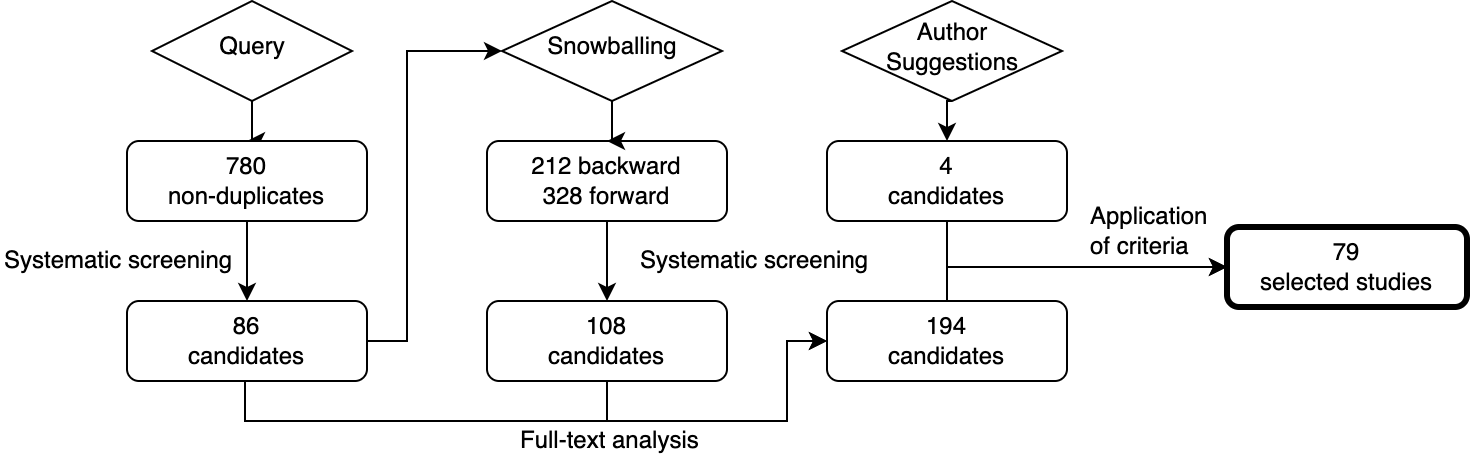
\includegraphics[width=0.8\linewidth]{slr_tight.png}
%  \caption{Diagram of the literature review process.}
%  \label{fig:literature_review}
%\end{figure}

%\newcommand{\rowselected}[6]{
\scriptsize \citetalias{#1} & % Citation alias
%\scriptsize \citep{#1} & % Standard citation
\scriptsize \citeyear{#1} & % Citation year
\scriptsize \nohyphens{\citet{#1}} & % Authors
\scriptsize #2 & % Full title
\scriptsize {\color{olive} #3} & % TCP
\scriptsize {\color{teal} #4} & % TCS
\scriptsize {\color{brown} #5} & % TSR
\scriptsize {\color{purple} #6} % TSA
\tabularnewline }

%\begin{table}[]

%\begin{center}
\rowcolors{3}{}{gray!10}
\setlength{\tabcolsep}{1.2pt}
\begin{longtable}{p{5mm}lp{22mm}p{90mm}llll}
\toprule
\scriptsize \textbf{ID} & 
\scriptsize \textbf{Year} & 
\scriptsize \textbf{Authors} & 
\scriptsize \textbf{Title} & 
\scriptsize \rotatedheader{olive}{\tcp} & 
\scriptsize \rotatedheader{teal}{\tcs} &
\scriptsize \rotatedheader{brown}{\tsr} &
\scriptsize \rotatedheader{purple}{\tsa}
\tabularnewline \midrule
%\input{tables/csv_selected.tex}

\rowselected{srikanth_requirements_2016}{Requirements Based Test Prioritization Using Risk Factors}{\fullcirc}{\emptycirc}{\emptycirc}{\emptycirc}
\rowselected{noor_similarity-based_2016}{A similarity-based approach for test case prioritization using historical failure data}{\fullcirc}{\emptycirc}{\emptycirc}{\emptycirc}
\rowselected{schwartz_cost-effective_2016}{Cost-effective regression testing through adaptive test prioritization strategies}{\fullcirc}{\emptycirc}{\emptycirc}{\emptycirc}
\rowselected{hirzel_graph-walk-based_2016}{Graph-walk-based selective regression testing of web applications created with Google web toolkit}{\emptycirc}{\fullcirc}{\emptycirc}{\emptycirc}
\rowselected{lu_how_2016}{How does regression test prioritization perform in real-world software evolution?}{\fullcirc}{\emptycirc}{\emptycirc}{\emptycirc}
\rowselected{vost_trace-based_2016}{Trace-based test selection to support continuous integration in the automotive industry}{\emptycirc}{\fullcirc}{\emptycirc}{\emptycirc}
\rowselected{wang_enhancing_2016}{Enhancing test case prioritization in an industrial setting with resource awareness and multi-objective search}{\fullcirc}{\emptycirc}{\emptycirc}{\emptycirc}
\rowselected{srikanth_test_2016}{Test Case Prioritization of Build Acceptance Tests for an Enterprise Cloud Application}{\fullcirc}{\emptycirc}{\emptycirc}{\emptycirc}
\rowselected{blondeau_test_2017}{Test case selection in industry: an analysis of issues related to static approaches}{\emptycirc}{\fullcirc}{\emptycirc}{\emptycirc}
\rowselected{pradhan_search-based_2016}{Search-Based Cost-Effective Test Case Selection within a Time Budget: An Empirical Study}{\emptycirc}{\fullcirc}{\emptycirc}{\emptycirc}
\rowselected{buchgeher_improving_2016}{Improving testing in an enterprise SOA with an architecture-based approach}{\fullcirc}{\fullcirc}{\emptycirc}{\emptycirc}
\rowselected{tahvili_dynamic_2016}{Dynamic integration test selection based on test case dependencies}{\fullcirc}{\fullcirc}{\emptycirc}{\emptycirc}
\rowselected{oqvist_extraction-based_2016}{Extraction-based regression test selection}{\emptycirc}{\fullcirc}{\emptycirc}{\emptycirc}
\rowselected{magalhaes_automatic_2016}{Automatic selection of test cases for regression testing}{\emptycirc}{\fullcirc}{\emptycirc}{\emptycirc}
\rowselected{aman_application_2016}{Application of Mahalanobis-Taguchi Method and 0-1 Programming Method to Cost-Effective Regression Testing}{\fullcirc}{\emptycirc}{\emptycirc}{\emptycirc}
\rowselected{busjaeger_learning_2016}{Learning for test prioritization: An industrial case study}{\fullcirc}{\emptycirc}{\emptycirc}{\emptycirc}
\rowselected{yoshida_fsx_2016}{FSX: A tool for fine-grained incremental unit test generation for C/C++ Programs}{\emptycirc}{\emptycirc}{\emptycirc}{\fullcirc}
\rowselected{tahvili_cost-benefit_2016}{Cost-benefit analysis of using dependency knowledge at integration testing}{\fullcirc}{\emptycirc}{\emptycirc}{\emptycirc}
\rowselected{ramler_tool_2017}{Tool support for change-based regression testing: An industry experience report}{\emptycirc}{\fullcirc}{\emptycirc}{\emptycirc}
\rowselected{strandberg_experience_2016}{Experience Report: Automated System Level Regression Test Prioritization Using Multiple Factors}{\fullcirc}{\fullcirc}{\emptycirc}{\emptycirc}
\rowselected{marijan_effect_2016}{Effect of time window on the performance of continuous regression testing}{\fullcirc}{\emptycirc}{\emptycirc}{\emptycirc}
\rowselected{gotlieb_using_2017}{Using global constraints to automate regression testing}{\emptycirc}{\emptycirc}{\fullcirc}{\emptycirc}
\rowselected{chi_multi-level_2017}{Multi-Level Random Walk for Software Test Suite Reduction}{\emptycirc}{\emptycirc}{\fullcirc}{\emptycirc}
\rowselected{bach_coverage-based_2017}{Coverage-Based Reduction of Test Execution Time: Lessons from a Very Large Industrial Project}{\fullcirc}{\fullcirc}{\emptycirc}{\emptycirc}
\rowselected{spieker_reinforcement_2017}{Reinforcement learning for automatic test case prioritization and selection in continuous integration}{\fullcirc}{\fullcirc}{\emptycirc}{\emptycirc}
\rowselected{vasic_file-level_2017}{File-Level vs. Module-Level Regression Test Selection for .NET}{\emptycirc}{\fullcirc}{\emptycirc}{\emptycirc}
\rowselected{celik_regression_2017}{Regression test selection across JVM boundaries}{\emptycirc}{\fullcirc}{\emptycirc}{\emptycirc}
\rowselected{ouriques_test_2018}{Test case prioritization techniques for model-based testing: a replicated study}{\fullcirc}{\emptycirc}{\emptycirc}{\emptycirc}
\rowselected{kwon_cost-effective_2017}{Cost-effective regression testing using bloom filters in continuous integration development environments}{\fullcirc}{\fullcirc}{\emptycirc}{\emptycirc}
\rowselected{garousi_multi-objective_2018}{Multi-objective regression test selection in practice: An empirical study in the defense software industry}{\emptycirc}{\fullcirc}{\emptycirc}{\emptycirc}
\rowselected{shi_evaluating_2018}{Evaluating test-suite reduction in real software evolution}{\emptycirc}{\emptycirc}{\fullcirc}{\emptycirc}
\rowselected{haghighatkhah_test_2018}{Test prioritization in continuous integration environments}{\fullcirc}{\emptycirc}{\emptycirc}{\emptycirc}
\rowselected{zhang_hybrid_2018}{Hybrid regression test selection}{\emptycirc}{\fullcirc}{\emptycirc}{\emptycirc}
\rowselected{miranda_fast_2018}{FAST Approaches to Scalable Similarity-Based Test Case Prioritization}{\fullcirc}{\emptycirc}{\emptycirc}{\emptycirc}
\rowselected{yilmaz_case_2018}{A case study to compare regression test selection techniques on open-source software projects}{\emptycirc}{\fullcirc}{\emptycirc}{\emptycirc}
\rowselected{chen_optimizing_2018}{Optimizing Test Prioritization via Test Distribution Analysis}{\fullcirc}{\emptycirc}{\emptycirc}{\emptycirc}
\rowselected{celik_regression_2018}{Regression Test Selection for TizenRT}{\emptycirc}{\fullcirc}{\emptycirc}{\emptycirc}
\rowselected{zhu_test_2018}{Test re-prioritization in continuous testing environments}{\fullcirc}{\emptycirc}{\emptycirc}{\emptycirc}
\rowselected{azizi_retest_2018}{Retest: A cost effective test case selection technique for modern software development}{\emptycirc}{\fullcirc}{\emptycirc}{\emptycirc}
\rowselected{guo_decomposing_2019}{Decomposing Composite Changes for Code Review and Regression Test Selection in Evolving Software}{\emptycirc}{\fullcirc}{\emptycirc}{\emptycirc}
\rowselected{zhong_testsage:_2019}{TestSage: Regression test selection for large-scale Web service testing}{\emptycirc}{\fullcirc}{\emptycirc}{\emptycirc}
\rowselected{fu_resurgence_2019}{Resurgence of Regression Test Selection for C++}{\emptycirc}{\fullcirc}{\emptycirc}{\emptycirc}
\rowselected{eda_efficient_2019}{An efficient regression testing approach for PHP Web applications using test selection and reusable constraints}{\emptycirc}{\fullcirc}{\fullcirc}{\emptycirc}
\rowselected{goyal_test_2019}{Test suite minimization of evolving software systems: A case study}{\emptycirc}{\emptycirc}{\fullcirc}{\emptycirc}
\rowselected{yu_terminator_2019}{TERMINATOR: better automated UI test case prioritization}{\fullcirc}{\emptycirc}{\emptycirc}{\emptycirc}
\rowselected{correia_motsd_2019}{MOTSD: A multi-objective test selection tool using test suite diagnosability}{\fullcirc}{\fullcirc}{\emptycirc}{\emptycirc}
\rowselected{machalica_predictive_2018}{Predictive Test Selection}{\emptycirc}{\fullcirc}{\emptycirc}{\emptycirc}
\rowselected{najafi_improving_2019}{Improving Test Effectiveness Using Test Executions History: An Industrial Experience Report}{\fullcirc}{\fullcirc}{\emptycirc}{\emptycirc}
\rowselected{leong_assessing_2019}{Assessing Transition-Based Test Selection Algorithms at Google}{\emptycirc}{\fullcirc}{\emptycirc}{\emptycirc}
\rowselected{cruciani_scalable_2019}{Scalable Approaches for Test Suite Reduction}{\emptycirc}{\emptycirc}{\fullcirc}{\emptycirc}
\rowselected{philip_fastlane:_2019}{FastLane: Test Minimization for Rapidly Deployed Large-Scale Online Services}{\emptycirc}{\emptycirc}{\fullcirc}{\emptycirc}
\rowselected{magalhaes_hsp_2020}{HSP: A hybrid selection and prioritisation of regression test cases based on information retrieval and code coverage applied on an industrial case study}{\fullcirc}{\fullcirc}{\emptycirc}{\emptycirc}
\rowselected{wu_time_2019}{A Time Window Based Reinforcement Learning Reward for Test Case Prioritization in Continuous Integration}{\fullcirc}{\emptycirc}{\emptycirc}{\emptycirc}
\rowselected{land_industrial_2019}{An Industrial Evaluation of Test Prioritisation Criteria and Metrics}{\fullcirc}{\emptycirc}{\emptycirc}{\emptycirc}
\rowselected{noemmer_evaluation_2020}{An Evaluation of Test Suite Minimization Techniques}{\emptycirc}{\emptycirc}{\fullcirc}{\emptycirc}
\rowselected{lubke_selecting_2020}{Selecting and Prioritizing Regression Test Suites by Production Usage Risk in Time-Constrained Environments}{\fullcirc}{\fullcirc}{\emptycirc}{\emptycirc}
\rowselected{yackley_simultaneous_2019}{Simultaneous refactoring and regression testing}{\emptycirc}{\fullcirc}{\emptycirc}{\emptycirc}
\rowselected{shi_understanding_2019}{Understanding and improving regression test selection in continuous integration}{\emptycirc}{\fullcirc}{\emptycirc}{\emptycirc}
\rowselected{lima_multi-armed_2022}{A Multi-Armed Bandit Approach for Test Case Prioritization in Continuous Integration Environments}{\fullcirc}{\emptycirc}{\emptycirc}{\emptycirc}
\rowselected{zhou_beating_2020}{Beating Random Test Case Prioritization}{\fullcirc}{\emptycirc}{\emptycirc}{\emptycirc}
\rowselected{peng_empirically_2020}{Empirically revisiting and enhancing IR-based test-case prioritization}{\fullcirc}{\emptycirc}{\emptycirc}{\emptycirc}
\rowselected{bertolino_learning--rank_2020}{Learning-to-rank vs ranking-to-learn: Strategies for regression testing in continuous integration}{\fullcirc}{\fullcirc}{\emptycirc}{\emptycirc}
\rowselected{chen_multi-objective_2021}{Multi-objective regression test selection}{\emptycirc}{\fullcirc}{\emptycirc}{\emptycirc}
\rowselected{zarges_artificial_2021}{An Artificial Immune System for Black Box Test Case Selection}{\emptycirc}{\emptycirc}{\emptycirc}{\emptycirc}
\rowselected{bagherzadeh_reinforcement_2022}{Reinforcement learning for test case prioritization}{\fullcirc}{\emptycirc}{\emptycirc}{\emptycirc}
\rowselected{elsner_empirically_2021}{Empirically evaluating readily available information for regression test optimization in continuous integration}{\fullcirc}{\fullcirc}{\emptycirc}{\emptycirc}
\rowselected{pan_dynamic_2020}{Dynamic Time Window based Reward for Reinforcement Learning in Continuous Integration Testing}{\fullcirc}{\emptycirc}{\emptycirc}{\emptycirc}
\rowselected{mehta_data-driven_2021}{Data-driven test selection at scale}{\emptycirc}{\fullcirc}{\emptycirc}{\emptycirc}
\rowselected{xu_requirement-based_2021}{A Requirement-based Regression Test Selection Technique in Behavior-Driven Development}{\emptycirc}{\fullcirc}{\emptycirc}{\emptycirc}
\rowselected{zhou_parallel_2022}{Parallel Test Prioritization}{\fullcirc}{\emptycirc}{\emptycirc}{\emptycirc}
\rowselected{sharif_deeporder_2021}{DeepOrder: Deep Learning for Test Case Prioritization in Continuous Integration Testing}{\fullcirc}{\emptycirc}{\emptycirc}{\emptycirc}
\rowselected{li_aga_2021}{AGA: An Accelerated Greedy Additional Algorithm for Test Case Prioritization}{\fullcirc}{\emptycirc}{\emptycirc}{\emptycirc}
\rowselected{chen_context-aware_2021}{Context-Aware Regression Test Selection}{\emptycirc}{\fullcirc}{\emptycirc}{\emptycirc}
\rowselected{zhang_comparing_2022}{Comparing and Combining Analysis-Based and Learning-Based Regression Test Selection}{\emptycirc}{\fullcirc}{\emptycirc}{\emptycirc}
\rowselected{abdelkarim_tcp-net_2022}{TCP-Net: Test Case Prioritization using End-to-End Deep Neural Networks}{\fullcirc}{\emptycirc}{\emptycirc}{\emptycirc}
\rowselected{cingil_black-box_2022}{Black-box Test Case Selection by Relating Code Changes with Previously Fixed Defects}{\emptycirc}{\fullcirc}{\emptycirc}{\emptycirc}
\rowselected{yaraghi_scalable_2022}{Scalable and Accurate Test Case Prioritization in Continuous Integration Contexts}{\fullcirc}{\emptycirc}{\emptycirc}{\emptycirc}
\rowselected{omri_learning_2022}{Learning to Rank for Test Case Prioritization}{\fullcirc}{\emptycirc}{\emptycirc}{\emptycirc}
\rowselected{greca_comparing_2022}{Comparing and combining file-based selection and similarity-based prioritization towards regression test orchestration}{\fullcirc}{\fullcirc}{\emptycirc}{\emptycirc}
\hiderowcolors
\midrule
& & & Totals & 46 & 41 & 8 & 1 
 \\ \bottomrule
\caption{Selected papers.}

%\\
%\hiderowcolors
%\bottomrule
%\caption{Selected papers.}
\label{table:selected}
\end{longtable}
%\end{center}

\setlength{\tabcolsep}{6pt}

%\begin{table}[]
%\centering
%\scriptsize
%\rowcolors{1}{}{gray!10}
%\begin{tabular}{llp{40mm}p{60mm}ll}
%\toprule
%\textbf{ID} & \textbf{Year} & \textbf{Authors} & \textbf{Title} & \textbf{Publisher} & \textbf{Ref.}  \\ \midrule
%%\input{tables/csv_selected_1.tex}
%%\rowselected{srikanth_requirements_2016}{Requirements Based Test Prioritization Using Risk Factors}{Elsevier}
%
%\bottomrule
%\end{tabular}
%%\caption{Selected papers.}
%\label{table:selected_1}
%\end{table}
%
%\begin{table}[]
%\centering
%\scriptsize
%\rowcolors{1}{}{gray!10}
%\begin{tabular}{llp{40mm}p{60mm}ll}
%\toprule
%\textbf{ID} & \textbf{Year} & \textbf{Authors} & \textbf{Title} & \textbf{Publisher} & \textbf{Ref.}  \\ \midrule
%\input{csv_selected_2.tex}
%\bottomrule
%\end{tabular}
%%\caption{Selected papers.}
%\label{table:selected_2}
%\end{table}
%
%\begin{table}[]
%\centering
%\scriptsize
%\rowcolors{1}{}{gray!10}
%\begin{tabular}{llp{40mm}p{60mm}ll}
%\toprule
%\textbf{ID} & \textbf{Year} & \textbf{Authors} & \textbf{Title} & \textbf{Publisher} & \textbf{Ref.}  \\ \midrule
%\input{csv_selected_3.tex}
%\bottomrule
%\end{tabular}
%\caption{Selected papers.}
%\label{table:selected_3}
%\end{table}

\subsection{Data Extraction}
\label{subsec:extraction}


To collect the data, each of the selected papers was assigned to one author to lead the data extraction, and to another author to review the data afterwards.
Thus, each paper was thoroughly reviewed by at least two authors.
At the end of this phase, the three authors performed a broad review of the collected information in order to ensure consistency of the results.

During the full-text analysis of the selected papers, we took notes of four groups of properties we wished to extract from each paper.
First, we wanted to have the core bibliographical information of the paper.
Then, we categorized the papers according to the \rt challenge being addressed and contextual factors such as software type and development environment.
We also took note of eight properties we considered important regarding \rea of each proposed technique or case study.
Finally, we synthesized the results of the papers by highlighting the types of approaches and metrics used and, if available, the open challenges/future work discussed by the authors.
The properties we collected are listed in \autoref{table:extraction}.

Some further explanation is needed regarding the ``applicability concerns'' properties.
During the data extraction, it became clear to us that there is some ambiguity regarding industrial motivation; among the non-selected papers, we also saw a great number of them briefly mentioning industry needs in the abstract and introduction, but not forming a connection between those needs and the technique being proposed.
So, for our criteria, industrial needs must not only be mentioned, but clearly stated with motivating evidence and/or references, and serve as the actual principle behind the idea of the study.

Regarding the industrial evaluation of results, this property is satisfied when experiments are performed directly on industrial software, usually through collaboration with a technology company.
However, there are plenty of papers that have robust experiments performed on notable open-source software, such as those from the Apache and Mozilla foundations.
Thus, we collect the following information about the subjects:
\begin{itemize}
	\item Its openness, which can be industrial proprietary, industrial open-source, fully open-source, or an academic dataset;
	\item Its testing scale (small up to 500 TCs, medium up to 2,000 TCs, large up to 10,000 TCs, or very large if more than that)\footnote{It is also important to note that the number of test cases is only one dimension of scale: on~\citetalias{cingil_black-box_2022}, for example, evaluation was performed on Smart TV apps with only 38 test cases, but the testing time was over 7 hours.};
	\item The language used for writing tests, which can be a programming language, natural language, a domain-specific language or a combination; and
	\item Its origin (the company that wrote it, or the dataset it is from).
\end{itemize}

We also checked to see if there is feedback from practitioners in the text of the paper.
Relatively few authors include feedback and, often times, it is only a brief passage.
Sometimes feedback seems to be implied, but we only considered explicit references to comments from practitioners (in either direct or indirect quotes).

The remaining properties are more straightforward:
For experiment subject(s) and industry partner, we merely point out the kind of software (or the specific software, if possible) used for evaluation, as well as any collaboration received from a company.
For industrial author(s), we check if the authors of the paper come from an academic, industrial or mixed background.
``Available tool'' is a URL pointing to an implementation of the technique, if it exists (regardless if it is source code, a plug-in, or a robust replication package).
Finally, ``put into practice'' indicates whether the technique was actually incorporated into the development workflow of a software, to the extent of the information contained in the paper.

Most of the data extracted according to the form can be found in this document under \autoref{table:selected} (bibliographical data); Figures \ref{fig:info_approaches} and \ref{fig:alg_approaches} (approaches); Figures \ref{fig:effectiveness_metrics} and \ref{fig:efficiency_metrics} (metrics); and Table \ref{table:relevance} (\rea relevance properties).
Additional properties, such as abstracts, DOIs, details on the experiment subjects, and links to supplementary material, can be found in the live repository.

%\newcommand{\rowextraction}[2]{
#1 & % Citation alias
#2 % Full title
\\ }
\newcommand{\rowextractionheader}[2]{
\textbf{#1} & % Citation alias
#2 % Full title
\\ }

\begin{table}[]
\centering
\scriptsize
\rowcolors{1}{}{gray!10}
\begin{tabular}{lp{0.8\textwidth}}
\toprule
%\textbf{Data} & \textbf{Description}  \\ \midrule
\rowextractionheader{Bibliographical data}{Basic information about the publication.}
\midrule
\rowextraction{Date}{The date the paper was made available online.}
\rowextraction{Authors}{The list of authors.}
\rowextraction{Title}{The title of the paper.}
\rowextraction{Abstract}{The abstract of the paper.}
\rowextraction{Venue and Publisher}{The conference or journal where it was published and its organization.}
\rowextraction{DOI}{The Digital Object Identifier of the paper.}
\midrule
\rowextractionheader{Categorization}{Details regarding the problem addressed by the paper.}
\midrule
\rowextraction{\rt challenges}{Whether the paper covers \tcp, \tcs, \tsr, \tsa or a combination.}
\rowextraction{Context}{The type of software targeted by the approach.}
\midrule
\rowextractionheader{Applicability concerns}{Properties of the paper related to its \rea.}
\midrule
\rowextraction{Industry motivation}{Whether the paper is clearly motivated by an industrially relevant problem.}
\rowextraction{Industry evaluation}{Whether the technique is evaluated in industrial software or sufficiently large-scale open-source projects.}
\rowextraction{Experiment subject(s)}{Which software or kind of software was used for the experimental evaluation of the technique, including the testing scale, the availability and the language in which tests are written.}
\rowextraction{Industry partner}{Which, if any, industrial partner collaborated with the development and/or evaluation of the technique.}
\rowextraction{Industrial author}{Whether one or more of the authors of the paper come from industry.}
\rowextraction{Practitioner feedback}{Whether practitioners were consulted to provide feedback to the results of the paper.}
\rowextraction{Available tool}{Whether the technique introduced in the paper is available to be used, either as a prototype or as a complete tool. If true, we also stored the relevant URLs.}
\rowextraction{Put into practice}{Whether the proposed tool has been adopted into the development process of a certain software.}
\midrule
\rowextractionheader{Findings}{Details of the proposed technique and remaining challenges.}
\midrule
\rowextraction{Approach}{What sort of algorithm and information the technique is using.}
\rowextraction{Metrics}{What criteria are being used for evaluating the techniques.}
\rowextraction{Open challenges}{What the authors list as next steps and unsolved issues related to the problem they addressed.}
\bottomrule
\end{tabular}
\caption{Data extraction form.}
\label{table:extraction}
\end{table}


\subsection{Questionnaire with Authors}
\label{subsec:questionnaires}

As we collected the data needed to answer the research questions, we realized the need of a perspective beyond what is possible to extract solely from the papers, particularly regarding the ongoing usage of the described techniques.
This happens because the information contained in the papers themselves might be out-of-date or unclear.
For example, the authors of~\citetalias{buchgeher_improving_2016} mention that their tool, TePSEx, was in use at the time of the publication; however, it is impossible to tell from the paper itself whether the situation has changed since 2016.
Conversely, there are also several papers that mention a practical implementation among their future work [\citetalias{wang_enhancing_2016}, 
\citetalias{tahvili_dynamic_2016}, 
\citetalias{gotlieb_using_2017}, 
\citetalias{celik_regression_2018}, 
\citetalias{philip_fastlane:_2019}], but we were not able to find follow-up papers clarifying whether that actually happened.

In order to provide a satisfactory answer to RQ3, we reached out to the authors of the papers via e-mail.
Our initial objective was to discover if techniques were ever put into practice and, if so, if they continue to be used to this day.
We also realized that the authors could also provide fruitful insight into RQ1 and RQ2, so it ultimately became an important pillar of this work.

We were able to contact authors from most of the papers; in some cases we were not able to locate the author's e-mail address, or the address is no longer valid.
The authors were given 12 days to respond and we received replies related to 51 out of the \numpapers papers --- in some cases, one author answered for several papers, in others several authors of the same paper provided answers.
The total number of responding authors was 45, although five of them did not provide meaningful answers (i.e. asked us to contact another co-author or said they were not able to answer our questions).

The e-mail sent out to the authors had the following questions:

\begin{tcolorbox}%[size=minimal]
\small
\begin{enumerate}
	\item  Is there a functional version of your technique (tool, prototype, source code, etc.) available online? If so, please share with us the URL.

	\item Was there an attempt to implement your technique in industrial or large open-source software? Is the technique currently in use with the software?

	\item If the technique was put into practice, were the metrics used in the paper relevant for the technique’s applicability? If not, were there other metrics that proved to be useful?
\end{enumerate}
\end{tcolorbox}

In addition, we also asked if the authors authorized their answers to be used in this study, if we could link them to their answers, and if they wish to be contacted about updates to this study.
All responding authors authorized the use of their answers, but several of them asked not to be linked directly to specific answers due to non-disclosure agreements with industrial partners; therefore, we use the received answers broadly, collecting quantitative and qualitative data from them without specifying which piece of information came from which author.
Whenever a direct quote is significant, we transcribe it anonymously; for readability we use an arbitrary ID numbering.

\subsection{Survey with Practitioners}
\label{subsec:prac_survey}

In addition to the questions we sent to the authors of reviewed papers, we also prepared a survey destined to practitioners.
The objective of this survey was to complement and verify some of the conclusions we draw from the literature, and help align the interests of academia and industry.

The survey was disseminated using a convenience sample, including contacts we personally know in industry and people who participated in software testing centric events.
We considered also putting the survey in public online forums centered on software testing/engineering, but ultimately decided against that for fear of low-quality responses and data pollution.

We received 23 responses from practitioners in six different countries (Brazil, Italy, Finland, Hungary, Portugal and Sweden). 
Obviously this survey covers an extremely small part of software testing practice, but it is possible to trace some common elements pointed out by the respondent that corroborate some of the findings and conclusions we had extracted from the literature.
When relevant, these responses are used in \autoref{sec:conclusions}.

Due to space concerns, we cannot include the full questionnaire here, but it is available online, along with the anonymized responses we received.
The main points covered in it were:
\begin{tcolorbox}%[size=minimal]
\small
\begin{enumerate}
	\item What are the most common pain points when it comes to regression testing?
	
	\item Do you know of, or have you ever used, a regression testing tool originating in academia?

	\subitem If so, how was the experience of using it?
	
	\item Do you stay informed on current advances in software engineering research? Are there attempts of collaboration between your company and academia?
	
\end{enumerate}
\end{tcolorbox}

We also asked their company, country and role, which we used to assess the diversity of respondents. This will not be published for privacy reasons.

\subsection{Replicability}
\label{subsec:replicability}

To allow replicability of our review and clearly describe the thought process behind the choice of included studies, we make a replication package available online\footnote{Available at: \url{https://bit.ly/3gCKh7V}.
For the purposes of review, we make the online material available through Google Sheets. This will be updated for the final release of the paper.}.
This package includes the original search queries, the list of papers that we included or excluded via the criteria, the full contents of the data extraction form, and the data used to generate the figures.
It also includes the full version of the e-mail template sent to the authors and the full questionnaire sent to practitioners.

%\section{State of the Art}\label{sec:lit_sota}

%\section{Live Repository}\label{sec:lit_live} 

\todo{spinoff as own chapter}

Literature reviews provide important information to researchers starting out in a field or practitioners who are curious to know the latest innovations, but do not have time to fully explore journals and conferences.
However, it is inevitable that a literature review such as this becomes outdated after some time, as new research comes out that cannot be included in the published paper.
This of course limits the long-term value of the work, since the text will no longer reflect the ongoing research in the field.

In order to aggregate long-term value to this work, we have made the list of papers and the information extracted from them available as an online live repository\footnote{Available at: \url{https://renangreca.github.io/literature-repository}.}.
The papers in \autoref{table:selected} serve as the starting point for a list that will continue to grow year over year.
We hope this website will serve as reference to anyone who is interested in practical applications of regression testing techniques in the coming years.

The main challenge is how to keep this repository alive in the long term.
It is unfeasible for us to add a relevant paper to the repository as soon as it is published, so our plan is to update the list in a yearly basis, re-running the query and screening steps detailed in \autoref{sec:methodology}.
That way, we can at least assure the most recent paper included is no more than one year old.
We are also looking into the possibility of getting automatic notifications when a paper that satisfies certain criteria is published in an online library.
For now, this work is done by the original authors of the literature review; according to future necessities, we will appoint other researchers or graduate students to help with the process.
In addition, we also encourage authors to submit their own work by filling a form linked on the website.

The repository also contains a separate section for relevant literature reviews.
This is initially populated by the reviews mentioned in \autoref{sec:related} and, upon publication, this very document.
With this we aim to provide a starting point for new researchers and a place to gather the overarching themes of the field.

It can also happen that, over the years, the definitions we selected for including a paper in the repository must be adjusted.
Whenever an author submits a paper, we will use the opportunity to consider whether or not the paper itself is a good fit for the repository, but also if there are new trends that our existing selection process does not account for.
There will likely be a point in the future when the industry/academia landscape has shifted and this study will no longer be needed.
When that happens, we will discuss the possibility of freezing the repository and stopping further expansions.

Aside from newer papers, it is always possible that we have missed some relevant papers for a variety of reasons, so the live repository is another way of mitigating that risk.
It is impossible to provide a complete and definitive overview of any field, but we believe that a live repository is the closest approximation that can be expected.

\todo{we want to keep the information summarized for future researchers/practitioners to gather data}

\todo{we want to keep it updated as to not need another systematic literature review on the same topic}

%\begin{figure}
%  \center
%  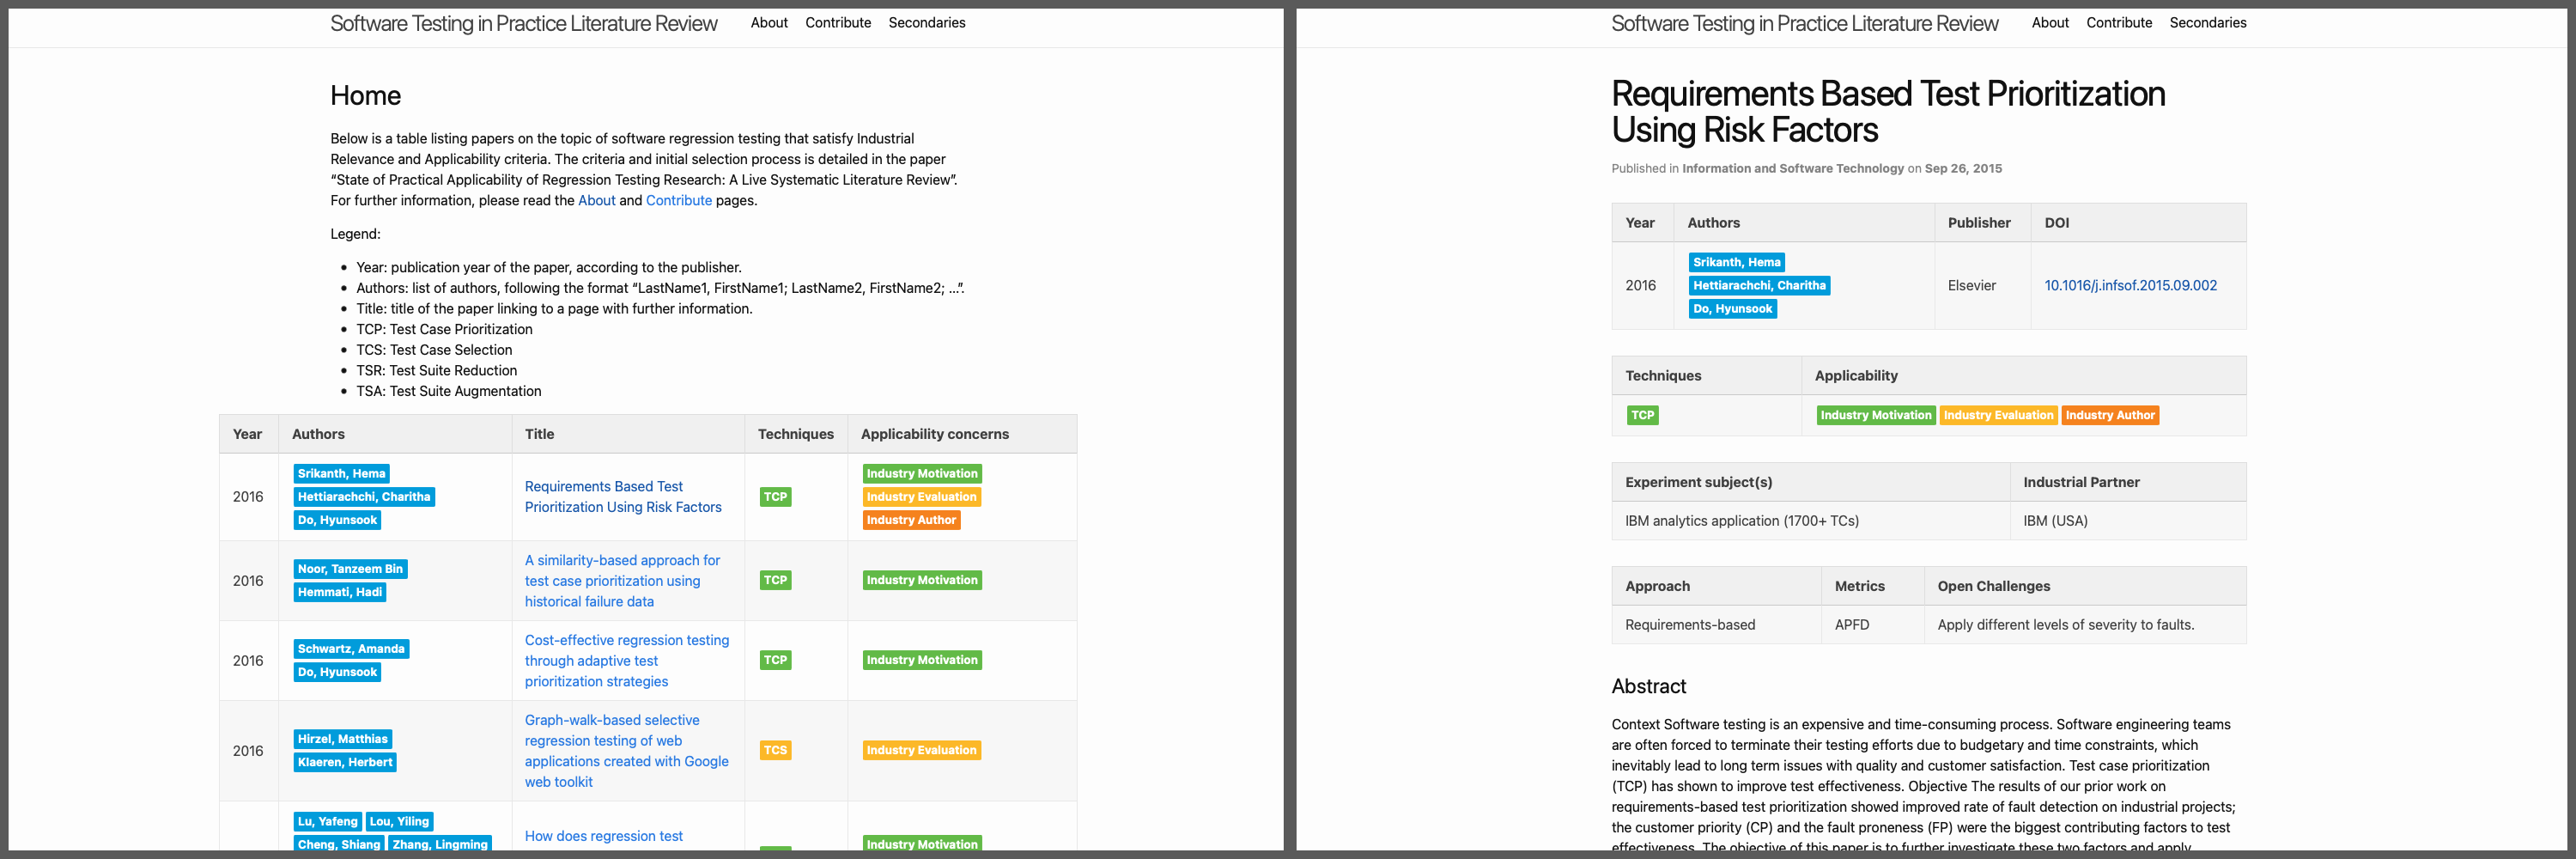
\includegraphics[width=\linewidth]{live_repository_screenshots_4.png}
%  \caption{Screenshots from the live repository. From left to right: 1) the main page listing the included papers; and 2) a single paper's page (\citetalias{srikanth_requirements_2016} used as example). }
%  \label{fig:live_repository}
%\end{figure}

\section{Discussion}\label{sec:lit_discussion}

\subsection{RQ1: Common Approaches and Metrics in \rt research}
\label{sec:lit_rq1}

A summary of the main approaches used to tackle \rt challenges is presented in \autoref{table:algo_approaches}.
We observe that the approaches adopted by a technique may serve to two different purposes:
one is regarding the source from where the information used as input for a technique is collected\footnote{This is also referred to as criteria in the literature~\citep{lou_survey_2018}.}; a second purpose refers to the actual algorithm used to address the problem to solve.
Correspondingly, the main approaches used to tackle \rt challenges are presented in \autoref{fig:info_approaches} and in \autoref{fig:alg_approaches}, respectively.
Regarding information, change-based, coverage-based, history-based and cost-aware approaches are the most common; while machine learning-based, search-based, similarity-based and graph-based are the popular algorithmic approaches.

%\newcommand{\rowapproach}[6]{
#1 & % Name
\textcolor{olive}{#2} & % TCP
\textcolor{teal}{#3} & % TCS
\textcolor{brown}{#4} & % TSR
\textcolor{purple}{#5} & % TSA
#6 % Description
\\}


\begin{figure}
  \center
  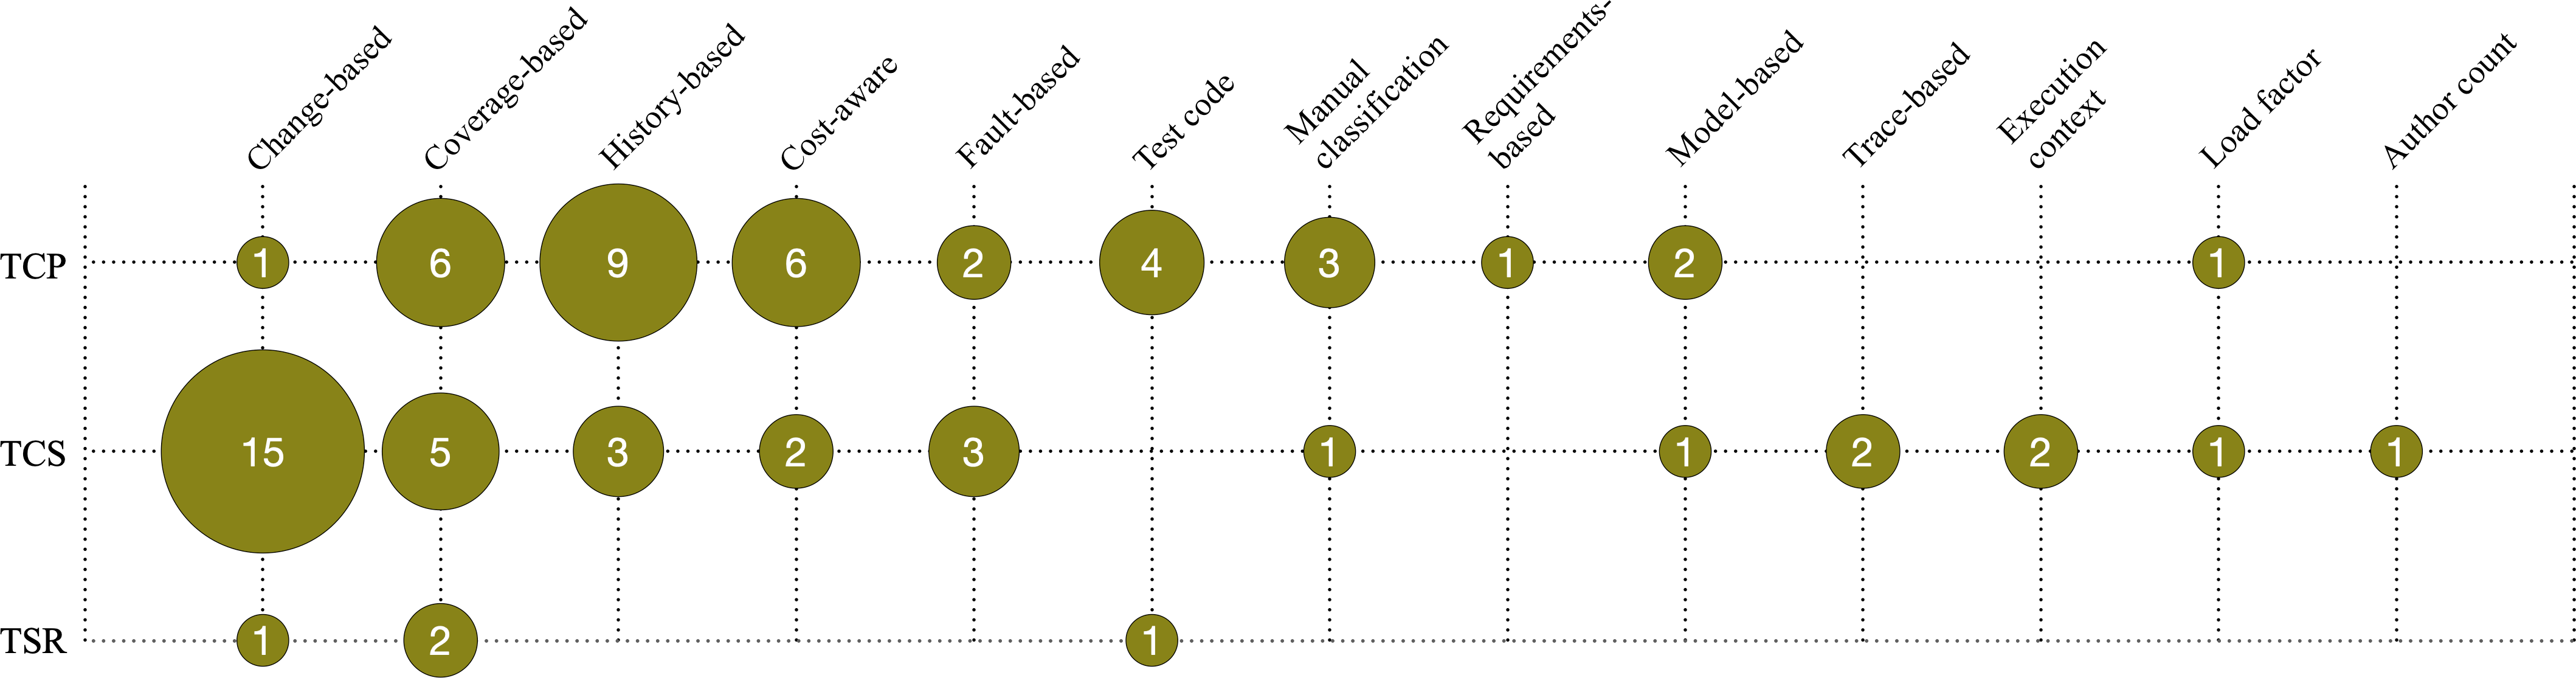
\includegraphics[width=\linewidth]{info_approach.png}
  \caption{Distribution of information approaches.}
  \label{fig:info_approaches}
\end{figure}

\begin{figure}
  \center
  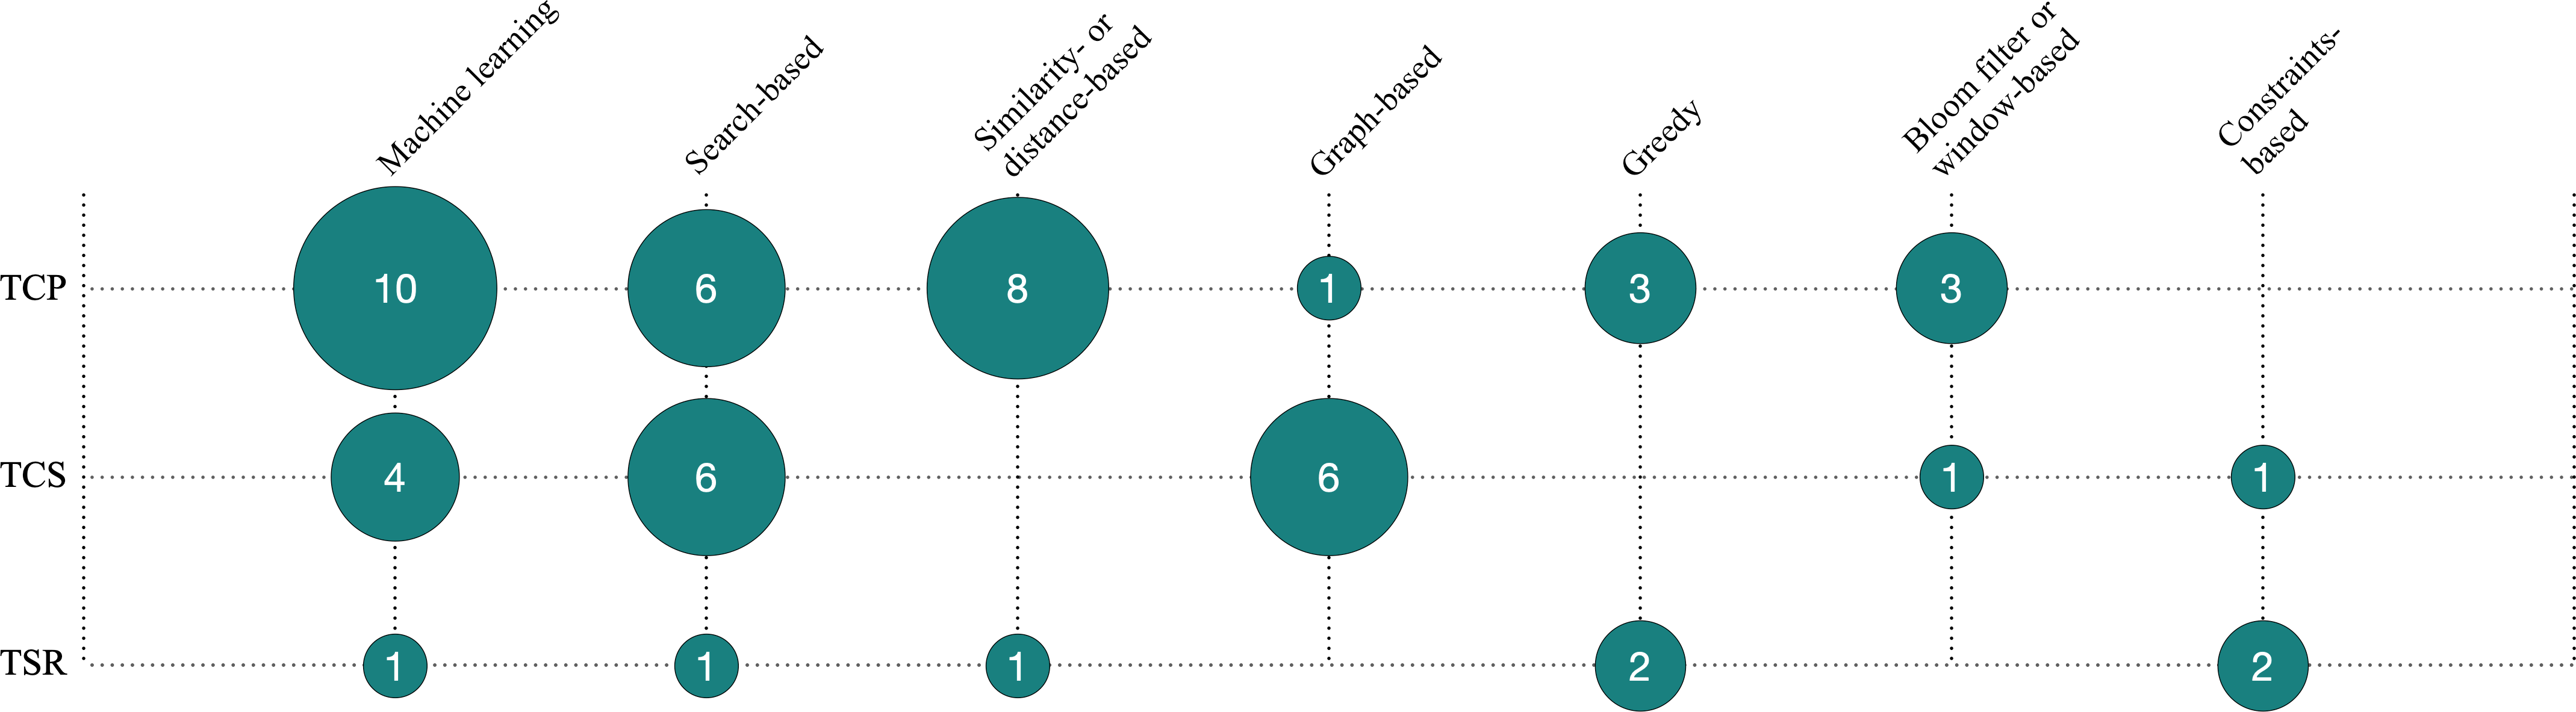
\includegraphics[width=\linewidth]{alg_approach.png}
  \caption{Distribution of algorithm approaches.}
  \label{fig:alg_approaches}
\end{figure}





\begin{table}[]
\scriptsize
\centering
\setlength{\tabcolsep}{1,2mm}
\begin{tabular}{p{23mm}p{18mm}p{18mm}p{8mm}p{3mm}p{55mm}}
\toprule
\textbf{Information} & 
\textcolor{olive}{\textbf{\tcp}} & 
\textcolor{teal}{\textbf{\tcs}} & 
\textcolor{brown}{\textbf{\tsr}} & 
\textcolor{purple}{\textbf{\tsa}} & 
\textbf{Description} \\ 
\midrule
%\rowcolors{1}{}{gray!10}
\showrowcolors
\input{tables/csv_approaches_information}
%\end{tabular}
%\caption{Information Approaches}	
%\label{table:info_approaches}
%\end{table}
%
%
%\begin{table}[]
%\scriptsize
%\centering
%\begin{tabular}{p{25mm}p{15mm}p{15mm}p{8mm}p{8mm}p{60mm}}
%\midrule
\textbf{Algorithm} & 
\textcolor{olive}{\textbf{\tcp}} & 
\textcolor{teal}{\textbf{\tcs}} & 
\textcolor{brown}{\textbf{\tsr}} & 
\textcolor{purple}{\textbf{\tsa}} & 
\textbf{Description} \\ 
\midrule
%\rowcolors{1}{}{gray!10}
\showrowcolors
\input{tables/csv_approaches_algorithm}
\end{tabular}
\caption{Information- and Algorithm-based Approaches}	
\label{table:algo_approaches}
\end{table}

%\begin{table}[]
%\scriptsize
%\centering
%\rowcolors{1}{}{gray!10}
%\setlength{\tabcolsep}{5pt}
%\begin{tabular}{c|p{15mm}|p{18mm}|p{18mm}|p{5.2mm}|p{5.3mm}|p{5.3mm}|p{50mm}}
%\toprule
% & \hspace{1mm} \textbf{Metric} & \textbf{\tcp} & \textbf{\tcs} & \textbf{\tsr} & \textbf{\tsa} & \textbf{Description} \\ 
%\midrule
%\rotatebox[origin=c]{90}{\textbf{Information}} &
%\multicolumn{6}{c}{
%%	\rowcolors{1}{}{gray!10}
%	\begin{tabular}{p{15mm}|p{18mm}|p{18mm}|p{5mm}|p{5mm}|p{50mm}}
%		\showrowcolors
%		\input{tables/csv_approaches_information}
%		
%
%	\end{tabular}
%}\\
%\midrule
%\rotatebox[origin=c]{90}{\textbf{Algorithm}} &
%\multicolumn{6}{c}{
%%	\rowcolors{1}{}{gray!10}
%	\begin{tabular}{p{15mm}p{18mm}p{18mm}p{5mm}p{5mm}p{50mm}}
%		\showrowcolors
%		\input{tables/csv_approaches_algorithm}
%		
%	\end{tabular}
%}\\
%
%\bottomrule
%
%\end{tabular}
%\caption{Approaches}	
%\label{table:approaches}
%\end{table}

The main metrics reported in the literature are shown in \autoref{table:other_metrics}, \autoref{fig:effectiveness_metrics} and \autoref{fig:efficiency_metrics}, grouped according to their main goal\footnote{In each figure, we omit \tsa due to space concerns, as only one paper~\citepalias{yoshida_fsx_2016} covers it.}.
The reported metrics primarily focus on effectiveness (how good a solution is at accomplishing its task) or efficiency (the time and cost of using the solution), but two metrics were identified that are neither --- namely, applicability/generality and diagnosability.

APFD is the most widely accepted metric for assessing \tcp{} approaches.
Because \tcs and \tsr both have the goal of running fewer tests than an original test suite, their metrics are mostly shared: testing time, selection count and fault detection ability are the most common ones.
The set of accuracy/precision/recall appears to be the effectiveness metric that covers the most situations.
For efficiency, the execution time of a technique is both widely used and is useful for any kind of solution.

%\newcommand{\rowmetric}[6]{
#1 & % Name
\textcolor{verdun}{#2} & % TCP
\textcolor{cyprus}{#3} & % TCS
\textcolor{derby}{#4} & % TSR
\textcolor{bossanova}{#5} & % TSA
#6 % Description
\\}

\begin{figure}
  \center
  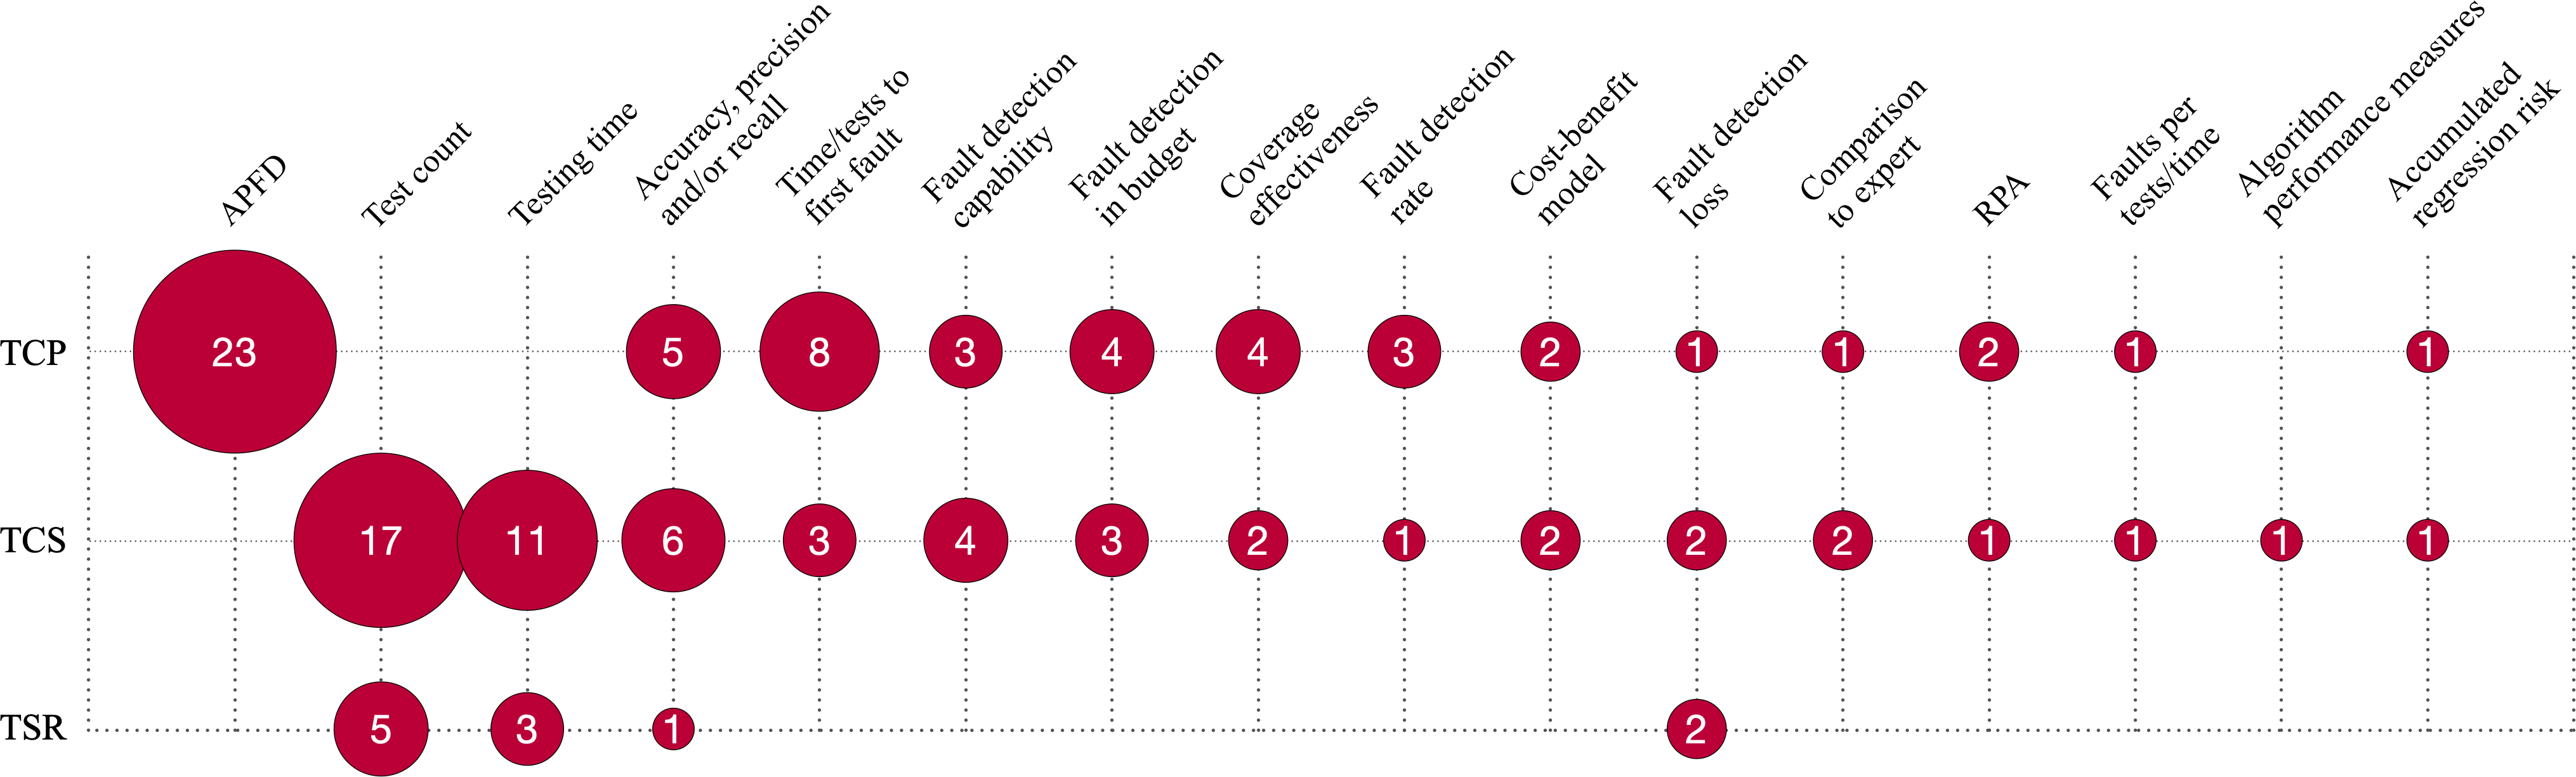
\includegraphics[width=\linewidth]{figures/effectiveness_metrics.pdf}
  \caption{Distribution of effectiveness metrics.}
  \label{fig:effectiveness_metrics}
\end{figure}

\begin{figure}
  \center
  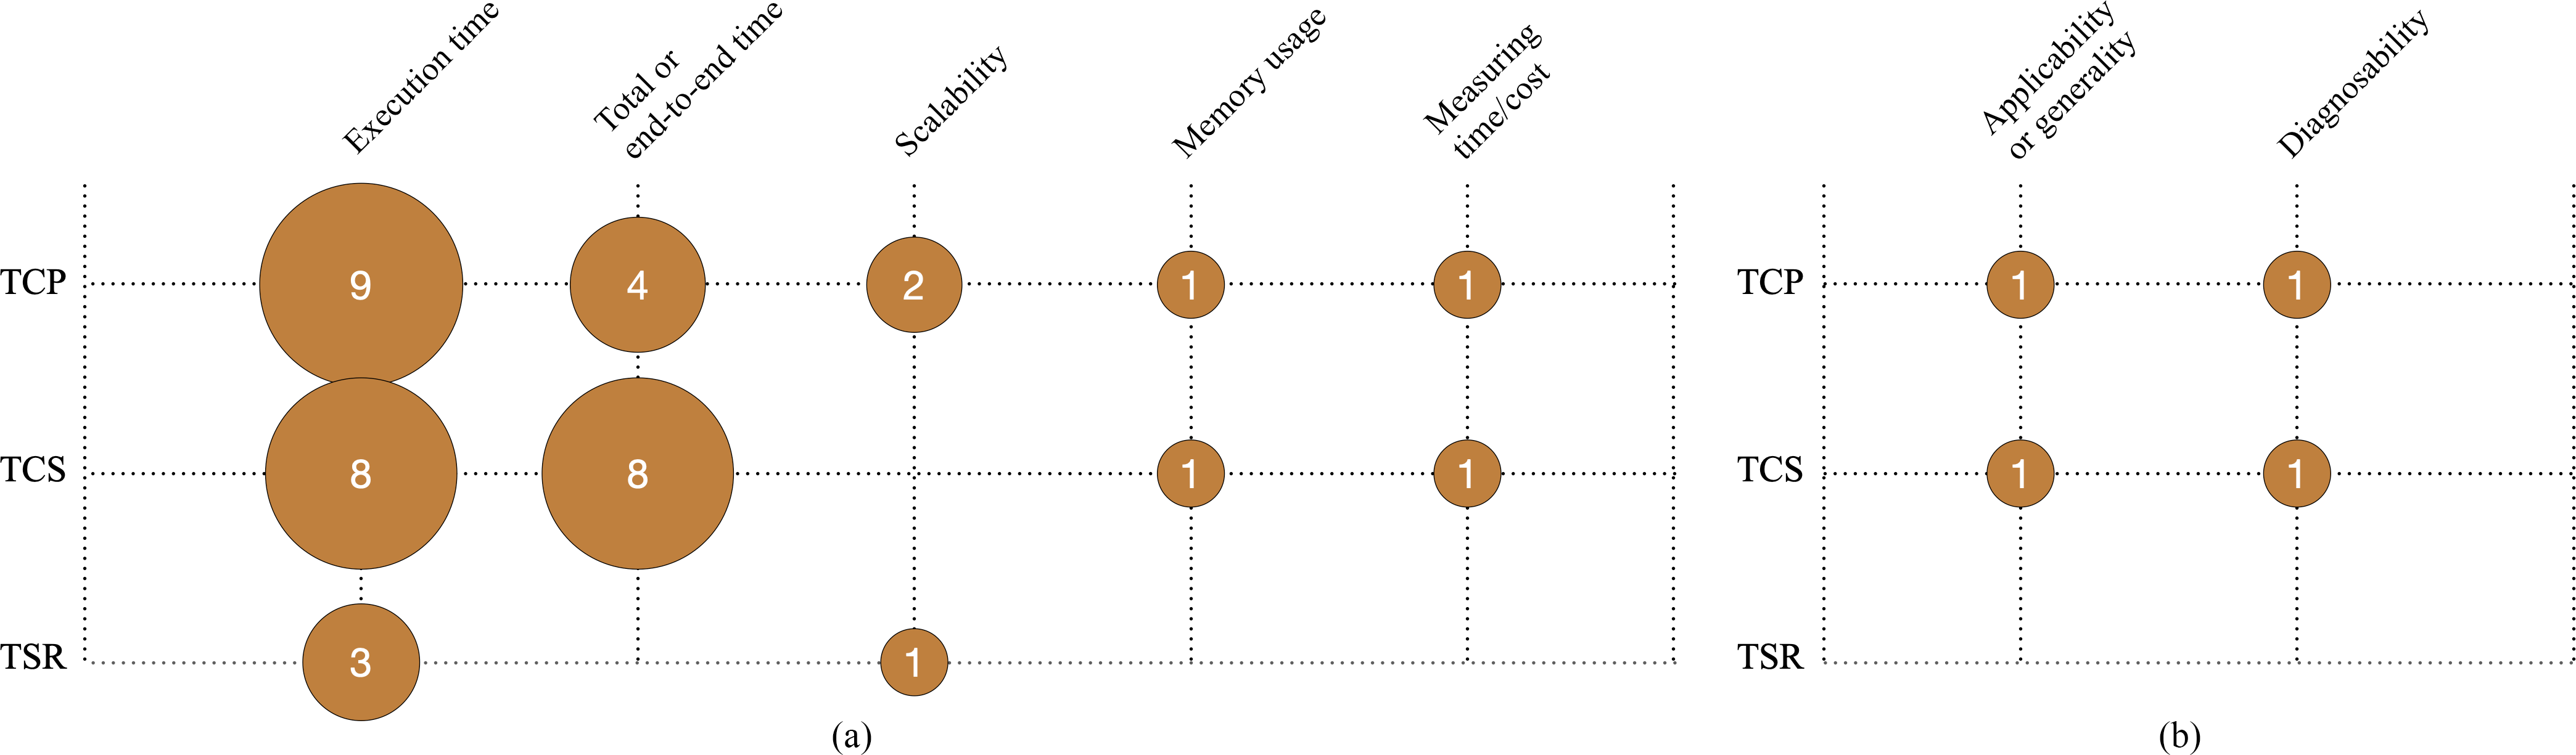
\includegraphics[width=\linewidth]{figures/efficiency_other_metrics.pdf}
  \caption{Distribution of (a) efficiency and (b) other metrics.}
  \label{fig:efficiency_metrics}
\end{figure}

\begin{table}[]
\scriptsize
\centering
\setlength{\tabcolsep}{1,2mm}
\begin{tabular}{p{23mm}p{18mm}p{18mm}p{8mm}p{8mm}p{60mm}}
\toprule
\textbf{Effectiveness} & 
\textcolor{verdun}{\textbf{\tcp}} & 
\textcolor{cyprus}{\textbf{\tcs}} & 
\textcolor{derby}{\textbf{\tsr}} & 
\textcolor{bossanova}{\textbf{\tsa}} & 
\textbf{Description} \\ 
\midrule
\showrowcolors
\input{tables/csv_metrics_effectiveness}
%\end{tabular}
%\caption{Effectiveness Metrics}	
%\label{table:effectiveness_metrics}
%\end{table}
%
%\begin{table}[]
%\scriptsize
%\centering
%\begin{tabular}{p{25mm}p{15mm}p{15mm}p{8mm}p{8mm}p{60mm}}
%\toprule
\textbf{Efficiency} & 
\textcolor{verdun}{\textbf{\tcp}} & 
\textcolor{cyprus}{\textbf{\tcs}} & 
\textcolor{derby}{\textbf{\tsr}} & 
\textcolor{bossanova}{\textbf{\tsa}} & 
\textbf{Description} \\ \midrule
\showrowcolors
\input{tables/csv_metrics_efficiency}
%\end{tabular}
%\caption{Efficiency Metrics}	
%\label{table:efficiency_metrics}
%\end{table}
%
%\begin{table}[]
%\scriptsize
%\centering
%\begin{tabular}{p{25mm}p{15mm}p{15mm}p{8mm}p{8mm}p{60mm}}
%\toprule
\textbf{Other} & 
\textcolor{verdun}{\textbf{\tcp}} & 
\textcolor{cyprus}{\textbf{\tcs}} & 
\textcolor{derby}{\textbf{\tsr}} & 
\textcolor{bossanova}{\textbf{\tsa}} & 
\textbf{Description} \\ \midrule
\showrowcolors
\input{tables/csv_metrics_other}
\end{tabular}
\caption{Effectiveness, Efficiency and Other Metrics}	
\label{table:other_metrics}
\end{table}

\setlength{\tabcolsep}{6pt}

%\begin{table}[h]
%\scriptsize
%\centering
%\begin{tabular}{cp{42mm}p{22mm}p{5.2mm}p{5.2mm}p{5.2mm}p{5.3mm}p{50mm}}
%\toprule
% & \hspace{1mm} \textbf{Metric} & \textbf{Referenced in} & \textbf{\tcp} & \textbf{\tcs} & \textbf{\tsr} & \textbf{\tsa} & \textbf{Description} \\ 
%\midrule
%
%\rotatebox[origin=c]{90}{\textbf{Effectiveness}} &
%\multicolumn{6}{c}{
%	\rowcolors{1}{}{gray!10}
%	\begin{tabular}{p{40mm}p{23mm}p{5mm}p{5mm}p{5mm}p{5mm}p{50mm}}
%	
%	\input{tables/csv_metrics_effectiveness}
%	
%	\end{tabular}
%}\\
%\midrule
%\rotatebox[origin=c]{90}{\textbf{Efficiency}} &
%\multicolumn{6}{c}{
%	\rowcolors{1}{}{gray!10}
%	\begin{tabular}{p{40mm}p{23mm}p{5mm}p{5mm}p{5mm}p{5mm}p{50mm}}
%	
%	\input{tables/csv_metrics_efficiency}
%		
%	\end{tabular}
%}\\
%\midrule
%\rotatebox[origin=c]{90}{\textbf{Other}} &
%\multicolumn{6}{c}{
%	\rowcolors{1}{}{gray!10}
%	\begin{tabular}{p{40mm}p{23mm}p{5mm}p{5mm}p{5mm}p{5mm}p{50mm}}
%	
%	\input{tables/csv_metrics_other}
%		
%	\end{tabular}
%}\\
%
%\bottomrule
%
%\end{tabular}
%\caption{Metrics}	
%\label{table:metrics}
%\end{table}

In our questionnaire to the authors, we included a question focused on the choice of metrics.
We asked authors who had successful or attempted attempts of implementing their technique whether the metrics described in the paper proved to be relevant in practice, or if additional measures were needed.
%
We received 27 meaningful responses to that question, out of which 24 were satisfied with the chosen metrics.
We quote some of the answers received:
``\textit{The metrics directly influenced decisions of the industrial partner}'' (respondent author \#16);
%
Respondent author \#8 stated that 
``\textit{[the] metrics were at the heart of the approach}'' 
and that the provided metrics were 
``\textit{always perceived as necessity by developers to support them in their work}'';
%
 ``\textit{The technique was put in practice for subsequent release and the metrics were useful and effective}'' (author \#17);
%
Respondent author \#23 answered that ``\textit{the metrics presented in the paper were critical for adoption and to measure ongoing improvements}'';
``\textit{they [the metrics] were relevant - they were also collected in the same environment in which the technique ended up being used}'' (author \#19).

Out of the three divergent responses, one suggested that the metrics were not a problem, but the dataset they used for the experiments was too small to provide meaningful evidence (author \#42).
Curiously, the remaining two complement each other. 
Author \#45 said that they proposed a new metric, which is believed to be relevant but has not been experimented in practice yet; while author \#25 claimed their own choice of metrics was not relevant to applicability, and is considering using the same metric proposed by \#45.


After analyzing all the answers to this question, two very interesting things emerged:
1) One author (\#14) reflected that although the metrics used were relevant at the time, looking back in retrospect other relevant metrics should have been used --- 
``\textit{Now, 7 years later, we have realized that some metrics were not included that should have been included}''.
The author was referring to the use of a metric for test case diversity as this could have helped them to tune the approach to avoid putting together many test cases targeting the same functionalities.
This reinforces the importance of following up the adoption of a proposed approach in its application environment:
even if we strive to anticipate all the possible uses of a proposed approach, observing its adoption in a real industrial context may reveal details and needs that were not captured while the approach was being conceived.
2) Two respondent authors (\#23 and \#36) reported that their approaches were evaluated with some additional metrics relevant to industry --- ``\textit{the company has also developed their own metrics}'' (respondent author \#36) --- that were not reported in their papers.
The answers do not make it clear if the metrics were omitted because the measurements were not available at the time the paper was published or if they were omitted on purpose (e.g., because they could reveal sensitive company data).

\begin{tcolorbox}%[size=fbox]
%\small
\textbf{Summary of RQ1.} The data reported in the figures show what are the most common approaches and metrics according to the objective of the \rt techniques. For example, we see that \tcp often relies on history-based and similarity-based approaches and uses APFD for evaluation, while \tcs is usually change-based with a focus on the number of selected tests.
We can also see that some overlap occurs and there are authors who choose unconventional but potentially promising combinations of techniques and metrics.
From the author responses we received, it appears that many authors are satisfied with their selection of metrics but a few indicate that more were discovered in the process of implementing the tool with their industrial partner.
\end{tcolorbox}


\subsection{RQ2: Applicability Concerns in Regression Testing Research}
\label{sec:lit_rq2}

%\newcommand{\rowrelevance}[7]{
\citetalias{#1} & % Citation alias
{\color{verdun} #2} & % Ind mot
{\color{cyprus} #3} & % Ind eval
{\color{derby} #4} & % Ind auth
{\color{bossanova} #5} & % Prac feed
{\color{diesel} #6} & % Avail tool
{\color{midnight} #7}   % In practice 
}

%\newcommand{\rotatedheaderfourtyfive}[2] {
%	\rotatebox[origin=c]{45}{\textbf{{\color{#1} #2}}}
%}

\newcommand{\relevanceheader} {
	\textbf{ID} & 
	\rotatedheader{verdun}{Ind. Mot.} &
	\rotatedheader{cyprus}{Ind. Eval.} &
	\rotatedheader{derby}{Ind. Auth.} &
	\rotatedheader{bossanova}{Prac. Feed.} &
	\rotatedheader{diesel}{Avail. Tool} &
	\rotatedheader{midnight}{In Practice}
}

%\begin{center}
%\scriptsize
%\rowcolors{3}{}{gray!10}
%\begin{longtable}{lllllll}
%\toprule
%\textbf{ID} & \textbf{Industrial} & \textbf{Industrial} & \textbf{Industrial} & \textbf{Practitioner} & \textbf{Available} & \textbf{Put into}  \\
%\textbf{} & \textbf{motivation} & \textbf{evaluation} & \textbf{author(s)} & \textbf{feedback} & \textbf{tool} & \textbf{practice} 
%\tabularnewline \midrule
%\input{tables/csv_relevance.tex}
%%\tabularnewline 
%%\hiderowcolors
%%\bottomrule
%%\caption{Relevance properties found in the papers.}
%\label{table:relevance}
%\end{longtable}
%\begin{center}
%\scriptsize
%\checkmark is used when the paper satisfies that property.\\ ? is used when it was not completely clear from the text if the property was satisfied or not.
%\end{center}
%\end{center}

%\begin{table}[]
%\scriptsize
%\centering
%\begin{tabular}{p{3mm}p{58mm}|p{3mm}p{58mm}}
%\toprule
%\textbf{ID} & \textbf{Properties} & \textbf{ID} & \textbf{Properties}\\ 
%\midrule
%\showrowcolors
%\input{tables/csv_relevance.tex}
%\end{tabular}
%\caption{Relevance properties found in the papers.}
%\scriptsize 
%{\color{olive} Ind. Mot.}: Industrial Motivation.
%{\color{teal} Ind. Eval.}: Industrial Evaluation.
%{\color{brown} Ind. Auth.}: Industrial Author(s).\\
%{\color{purple} Prac. Feed.}: Practitioner Feedback.
%{\color{orange} Avail. Tool}: Available Tool.
%{\color{cyan} In Practice}: Put into Practice.
%\label{table:relevance}
%\end{table}

\begin{table}[]
\scriptsize
\begin{center}
\rowcolors{2}{}{gray!10}
\setlength{\tabcolsep}{2pt}
\begin{tabular}{l llllll | l llllll | l llllll | l llllll}% | l llllll}
\toprule
\relevanceheader & \relevanceheader & \relevanceheader & \relevanceheader \\ 
\midrule
\input{tables/csv_relevance_4.tex}
\end{tabular}
\end{center}
\scriptsize 
\vspace{-9pt}
\textbf{\color{verdun} Ind. Mot.}: Industrial Motivation.
\textbf{\color{cyprus} Ind. Eval.}: Industrial Evaluation.
\textbf{\color{derby} Ind. Auth.}: Industrial Author(s).
\textbf{\color{bossanova} Prac. Feed.}: Practitioner Feedback.
\textbf{\color{diesel} Avail. Tool}: Available Tool.
\textbf{\color{midnight} In Practice}: Put into Practice.
%
A half-filled circle indicates a partially satisfied property. For example, a paper that provides its dataset but not its source code, or one that has some indication of having been implemented without explicitly stating so.
\caption{Relevance properties found in the papers.}
\label{table:relevance}
\end{table}

\setlength{\tabcolsep}{6pt}


To answer this research question, we look carefully at the applicability concerns extracted according to \autoref{table:extraction}.
The full mapping of the papers with the properties they satisfy is available in \autoref{table:relevance}.
It is worth observing that our conclusions here, as well as in the next section, are only relative to the set of primary studies that we retrieved; we cannot exclude the possibility that works that we did not select could eventually find application in practice.
For instance, a paper with no obvious practical motivation could be the theoretical foundation for a tool later adopted by practitioners.

Most of the selected papers satisfy the properties of having a clear industrial motivation: out of the \numpapers papers, only five~
[\citetalias{hirzel_graph-walk-based_2016}, 
\citetalias{aman_application_2016},
\citetalias{spieker_reinforcement_2017},  
\citetalias{yackley_simultaneous_2019}, 
\citetalias{shi_understanding_2019}] did not have a clear \rea motivation.
Regarding evaluation, 50 of the papers contained experiments on industrial (or industrial-scale) software.
In other words, it is quite clear that \rea is frequently a concern that motivates researchers to develop novel \rt techniques.
While providing adequate experimentation and evaluation to these techniques can be a tough challenge, it is one that researchers are indeed attempting to address.

Out of the 74 papers with relevant evaluation, 44 perform experiments with the direct collaboration of an interested partner --- in most cases a corporation, in one case a government department~\citepalias{garousi_multi-objective_2018}, indicating that such collaborations can play an important role in improving the relevance of experiments.
Curiously, there are also four papers that have industrial collaborations, but the experiments are not performed with software from that partner~
[\citetalias{yoshida_fsx_2016}, 
\citetalias{celik_regression_2017}, 
\citetalias{guo_decomposing_2019}, 
\citetalias{noemmer_evaluation_2020}].
Finally, there is one paper with an industrial partner but the objective of the work was not to develop a tool, so there are no experiments~\citepalias{land_industrial_2019}.

In our retrieved literature, the industrial background of the authors is significant in a few ways.
The papers with primarily industrial authors are the most likely ones to be relevant in practice, because these are generally designed with the application on a specific software product in mind; these papers usually provide insight into the testing workflow at large companies and share the lessons learned from applying a certain technique to a specific scenario.
Examples include \citetalias{machalica_predictive_2018} with Facebook; \citetalias{leong_assessing_2019} with Google and \citetalias{philip_fastlane:_2019} with Microsoft. There are also some cases of companies whose main product is not software, but software is an important part of their products (e.g., transportation manufacturers, as \citetalias{vost_trace-based_2016} with BMW).

Papers with a mix of industrial and academic authors also represent good progress in enhancing industry-academia collaborations, such as the collaborations between University of Texas at Austin and Microsoft [\citetalias{vasic_file-level_2017}, \citetalias{celik_regression_2018}] or between the Federal University of Pernambuco and Motorola \citepalias{magalhaes_automatic_2016, magalhaes_hsp_2020}.

Finally, we want to highlight the papers that have tools available online.
This is important for replicability and ease of access, but is still lacking in many publications.
To facilitate comparisons by other researchers and simplify experimentation by software developers, it is fundamental that a version of the technique exists, either in binary or source code format.
Only 22 of the surveyed papers made their tool available in some form (usually source code repository), making it improbable that any of the other tools were used by practitioners without direct contact with their developers.
Notably, there appears to be a change in this trend: between 2016 and 2020, only 14 papers had any sort of replication package or tool available.
In 2021 and 2022 (up until July), we found 8 papers satisfying this criteria.
The likely explanation to this is that noteworthy Software Engineering conferences have given more value to easily-replicable research in recent years and this has caused authors to make it a priority.
However, there are some cases where the code is made available with little to no documentation or explanation of how it works; on the bright side, there are also examples that stood out for having clear and detailed steps on how to use the code and replicate the experiments.
Among the e-mail responses from the authors, we received the source code repository URL for four additional papers, confirming that at least 26 papers have material available online --- whenever possible, the relevant URLs can be found in our live repository (\autoref{sec:repository}).

Out of the investigated URLs, only \citetalias{hirzel_graph-walk-based_2016} and \citetalias{zhang_hybrid_2018} provide clear usage instructions for arbitrary software projects; they are available as plug-ins for the Eclipse IDE and the Maven build system, respectively.
\citetalias{guo_decomposing_2019} also mentions the tool is available as an Eclipse plug-in, but we were unable to find a URL pointing to it.
The remaining papers provide their source code primarily for study replication, not necessarily intended for actual usage by developers, meaning that the tool is likely not sufficiently robust for practical usage beyond experiments.
It also happens frequently that tools developed in conjunction with an industrial partner end up becoming proprietary software and cannot be easily distributed (e.g. \citetalias{magalhaes_automatic_2016}, \citetalias{busjaeger_learning_2016}).
Authors of 14 papers said in their responses that the code or the tool could not be shared, since the resulting software is completely or partially proprietary or confidential.

An issue we identified is regarding the programming languages of the SUTs targeted by the experiments.
\autoref{fig:programming_languages} shows that there is a heavy bias towards Java, with 23 papers targeting software written in that language.
On most of the papers focused on a specific language, it is not clear if the same approach would be easy to adapt and would produce equivalent results on software developed using other widely used languages.
However, 12 papers target systems written in multiple languages, or explicitly state that the approach is language-agnostic, which highly increases its applicability.
Unfortunately, it was not possible to identify the target language of 21 papers; this creates a substantial challenge for both the replicability of the experiments and applicability of the technique.


%\begin{figure}
%  \center
%  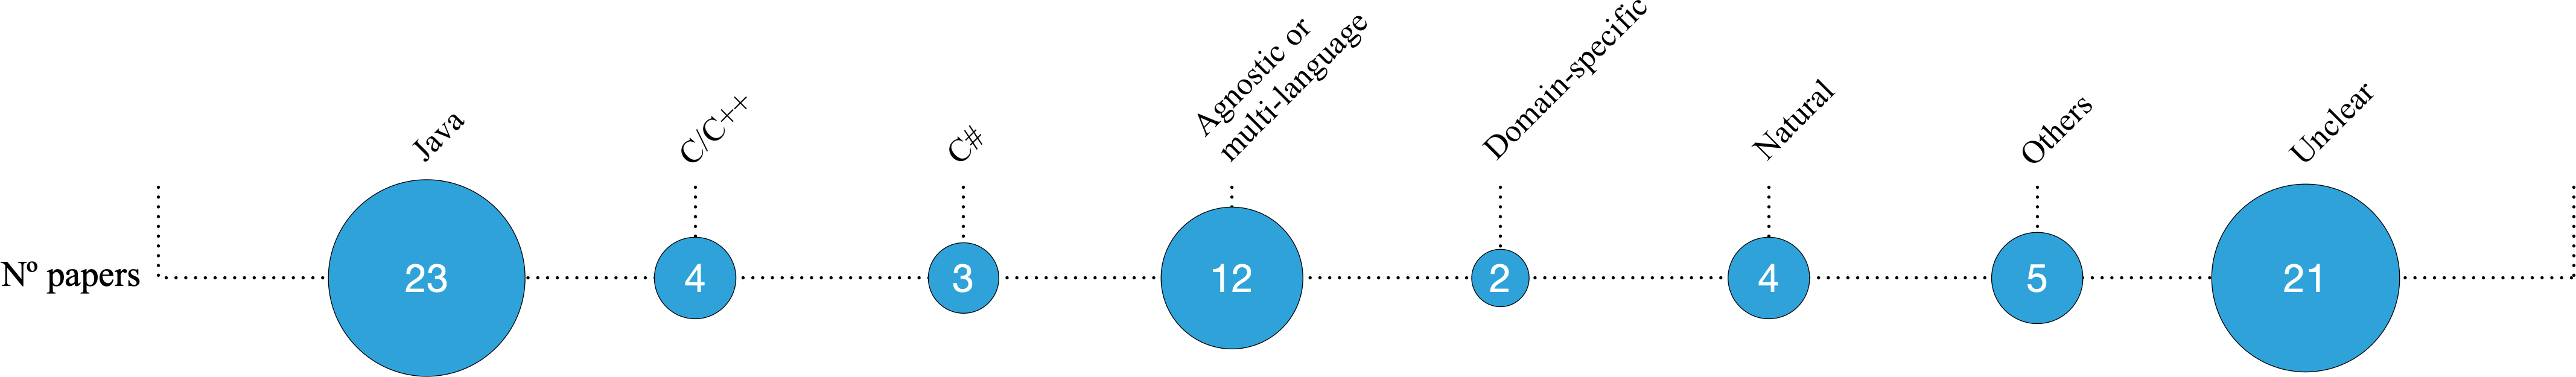
\includegraphics[width=\linewidth]{programming_languages.png}
%  \caption{Distribution of the targeted programming languages.}
%  \label{fig:programming_languages}
%\end{figure}


\begin{tcolorbox}%[size=fbox]%[boxsep=0mm,boxrule=0mm,size=minimal]
%\small
\textbf{Summary of RQ2.}
Our survey shows that a large number of papers exhibit \rea concerns in their motivations, and a smaller albeit still significant amount contains experiments at relevant scale. 
Most of the times, the techniques that are implemented into a software workflow are also papers that have authors from an industrial background. %while transferal of approaches that stem purely from academia still remains a challenge.
Unfortunately, few authors share their tools in a well-documented, open-source fashion, which hampers both future researchers, who wish to compare their solutions against the state-of-the-art, and practitioners, who might want to see how existing \rt tools can help their software.
\end{tcolorbox}






\subsection{RQ3: Evidences of Real-world Application of Regression Testing Techniques}
\label{sec:lit_rq3}

Our study is motivated by the concern that there is potentially valuable technology being proposed in academia that does not always make its way into usage in industry.
The difference between the state-of-the-art techniques proposed in academia and the ones actually used in real-world software is what we call the \emph{academia-industry technology transfer gap}.
Expressing concerns over \rea of \rt techniques is an important step towards awareness of the gap, although not sufficient \textit{per se} to solve the problem of actually putting these techniques into practice.
The focus of this section is to discover if and how much evidence exists of techniques developed by the research community being adopted by real-world software development.
As previously stated, there might be studies that have been put into practice, but escaped our review because they were not explicitly motivated by \rea; we hope that, in the future, our live repository solution will eventually find them and potentially widen the conclusions described here.

\autoref{table:relevance} contains only data extracted from the papers themselves; since the author responses are anonymous, we cannot map them directly to the table.
Thus,~\autoref{fig:relevance_count} displays the total number of papers that satisfy each of our applicability criteria, including updates from the author responses.
In other words, we consider the author response if it updates the information retrieved from the paper; otherwise the data extracted from the paper remains.

%\begin{figure}
%  \center
%  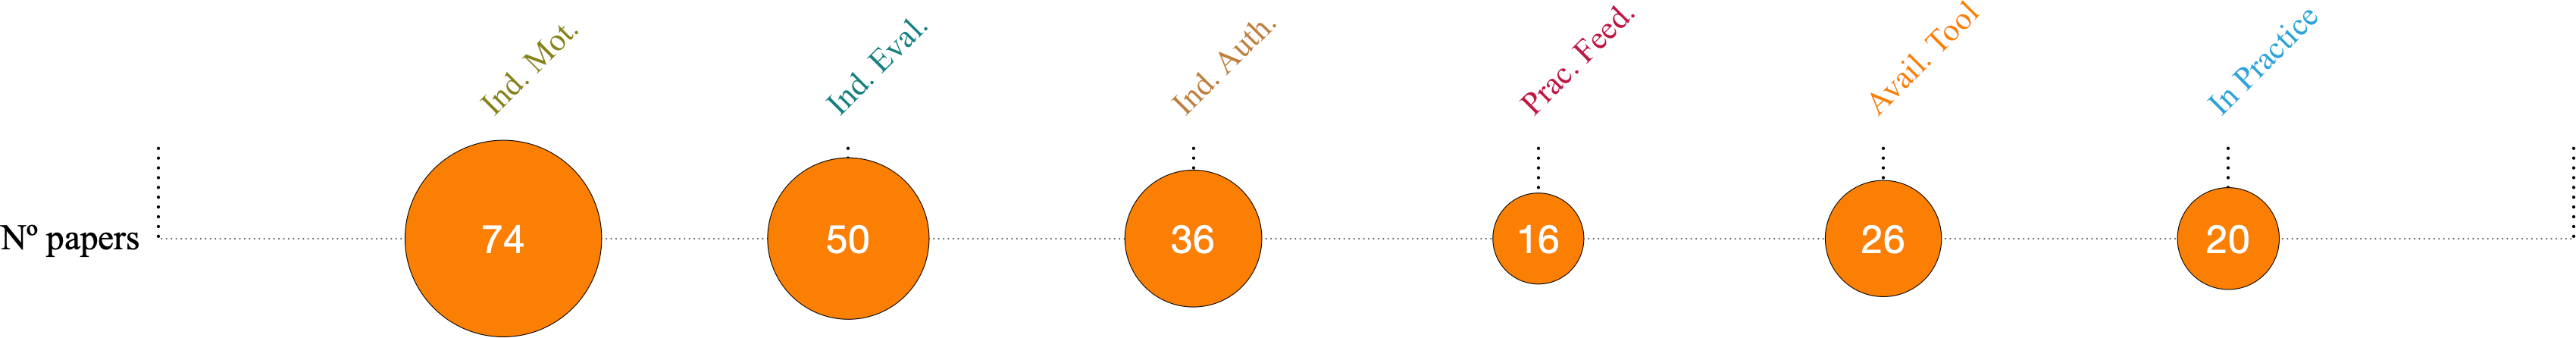
\includegraphics[width=\linewidth]{relevance_count.png}
%  \caption{Quantitative analysis of the satisfied criteria.}
%  \label{fig:relevance_count}
%\end{figure}


Regarding the adoption of the proposed approaches, \autoref{table:relevance} shows that 16 out of the \numpapers selected papers explicitly state that the proposal is applied with a partner, or suggest that implementation was ongoing at the time of publication, out of which six are confirmed to still be in use by their authors, while four say it fell out of use (the remaining six did not respond, so we assume no change).
Eight other authors claim their approach was implemented after publication, so the count in~\autoref{fig:relevance_count} is 20 (16-4+8).

We can observe that having a practitioner as a co-author helps to provide a direct line from the founding theory of the technique to its application in practice: 
indeed, 14 of these 20 papers have at least one author from industry.
This is not surprising, because such collaborations often originate directly from a need expressed by the practitioners.

However, we also see that only 8 out of those 20 papers featured feedback from the practitioners who actually used the developed tool.
That is, although the tool was incorporated into the production workflow, in many cases an assessment of long-term benefits and acceptance by its users is either not done or not reported.
%
Ultimately, the authors were our best chance of understanding the story behind each tool, revealing whether it is still being used by a partner and the reasons it might have fallen out of use.

From the respondent authors, we received six confirmations that the tool continues to be in use by their industrial partner in some form, e.g. ``\textit{The tool was implemented at a company [...] and it is still in use at the company [with significant changes].}'' from respondent author \#14.
Authors of another two papers stated that the technique is undergoing an implementation process at the time of the response.
Author \#37 claims that their work on a newer paper is seeing adoption by an industrial partner; however, at the time of writing, that paper remains in pre-print and cannot be formally included in this review.

Interestingly, eight authors say that the tool was successfully incorporated into an industrial partner's development cycle after the publication of the paper: ``\textit{the technique has been adapted and embedded into a random data selection tool by the [company]’s testing team, for purposes including but not limited to regression testing.}'' (author \#36); ``\textit{the [technique] has been in use at [company since roughly the date of publication. [It] is used to run relevant test cases for every code review in [company]'s main code repository.}'' (author \#23).
However, the details are not always known to them: ``\textit{We were told it was put into practice but we were not given any information, due to confidentiality rules.}'' (author \#44).

To the extent of the authors' knowledge, 12 papers were never put in practice, although some say there was a discussion to do so at some point.
From author \#35: ``\textit{We discussed the possibility of conducting a research visit at one of the corporation branches to experiment with the technique} in vivo\textit{, but in the end it did not go through.}''

Authors of ten papers (out of which four were tagged as implemented in~\autoref{table:relevance}) said that the tool saw usage but fell out of use after a few years; an additional three claimed some sort of attempt, but the current status is unknown.
What this means is that, even if a technique is incorporated into a software, a lot of work must still be done to ensure that the approach remains viable in a longer term.
Some challenges mentioned by these authors include:

\paragraph{The tool became outdated and it was not updated to remain relevant}
``\textit{It was implemented in an industrial setting, but this work is several years old and has to be evolved to stay relevant for business.}'' (author \#20).
This can be either due to a technical issue, e.g. the tool was designed for an older version of a programming language or platform and would require some effort to be updated and be used on newer software, or because the tool does not consider newer requirements of its subject software.

\paragraph{The authors noticed that adapting an academic prototype into an industry-strength tool required more time and budget than the project permitted}
``\textit{There is a gap between developing a research prototype and an industrial-strength tool. Evolving research prototypes towards industry-ready tools was beyond the project budget.}''(author \#8)
It can happen that a technique seems promising in initial experiments, but an enormous amount of work would be needed to actually incorporate it into a workflow.
The technique might require data that is not currently being collected, or use some manual process for the evaluation that would need to be automated.
The tool must also be verified for correctness and robustness before practical usage.

\paragraph{Authors lost contact with their partners and no longer follow development of the tool}
``\textit{[The tool] was supported by [our partner]. We have no input if the tool has been used.}'' (author \#26)
There are cases where the partnership does not continue after the publication of the paper or some other condition occurs.
The industrial partner is likely free to continue using the developed tool, but the authors from the academic side are no longer part of its evolution and do not receive updates and feedback regarding the subsequent challenges and achievements.

\paragraph{The cost-benefit ratio was off}
``\textit{We tried to use it within [our partner]. It seemed to work fine but the cost associated with the 1\% bugs that were missed is too high.}'' (author \#43)
Even if a \tcs technique detects 99\% of bugs by running a very small set of tests, practitioners will be skeptical of using as a replacement for TestAll strategy.
After all, although testing is a costly procedure, it is still much cheaper to detect an error during testing than after the software has been shipped to customers.

%\begin{figure}
%  \center
%  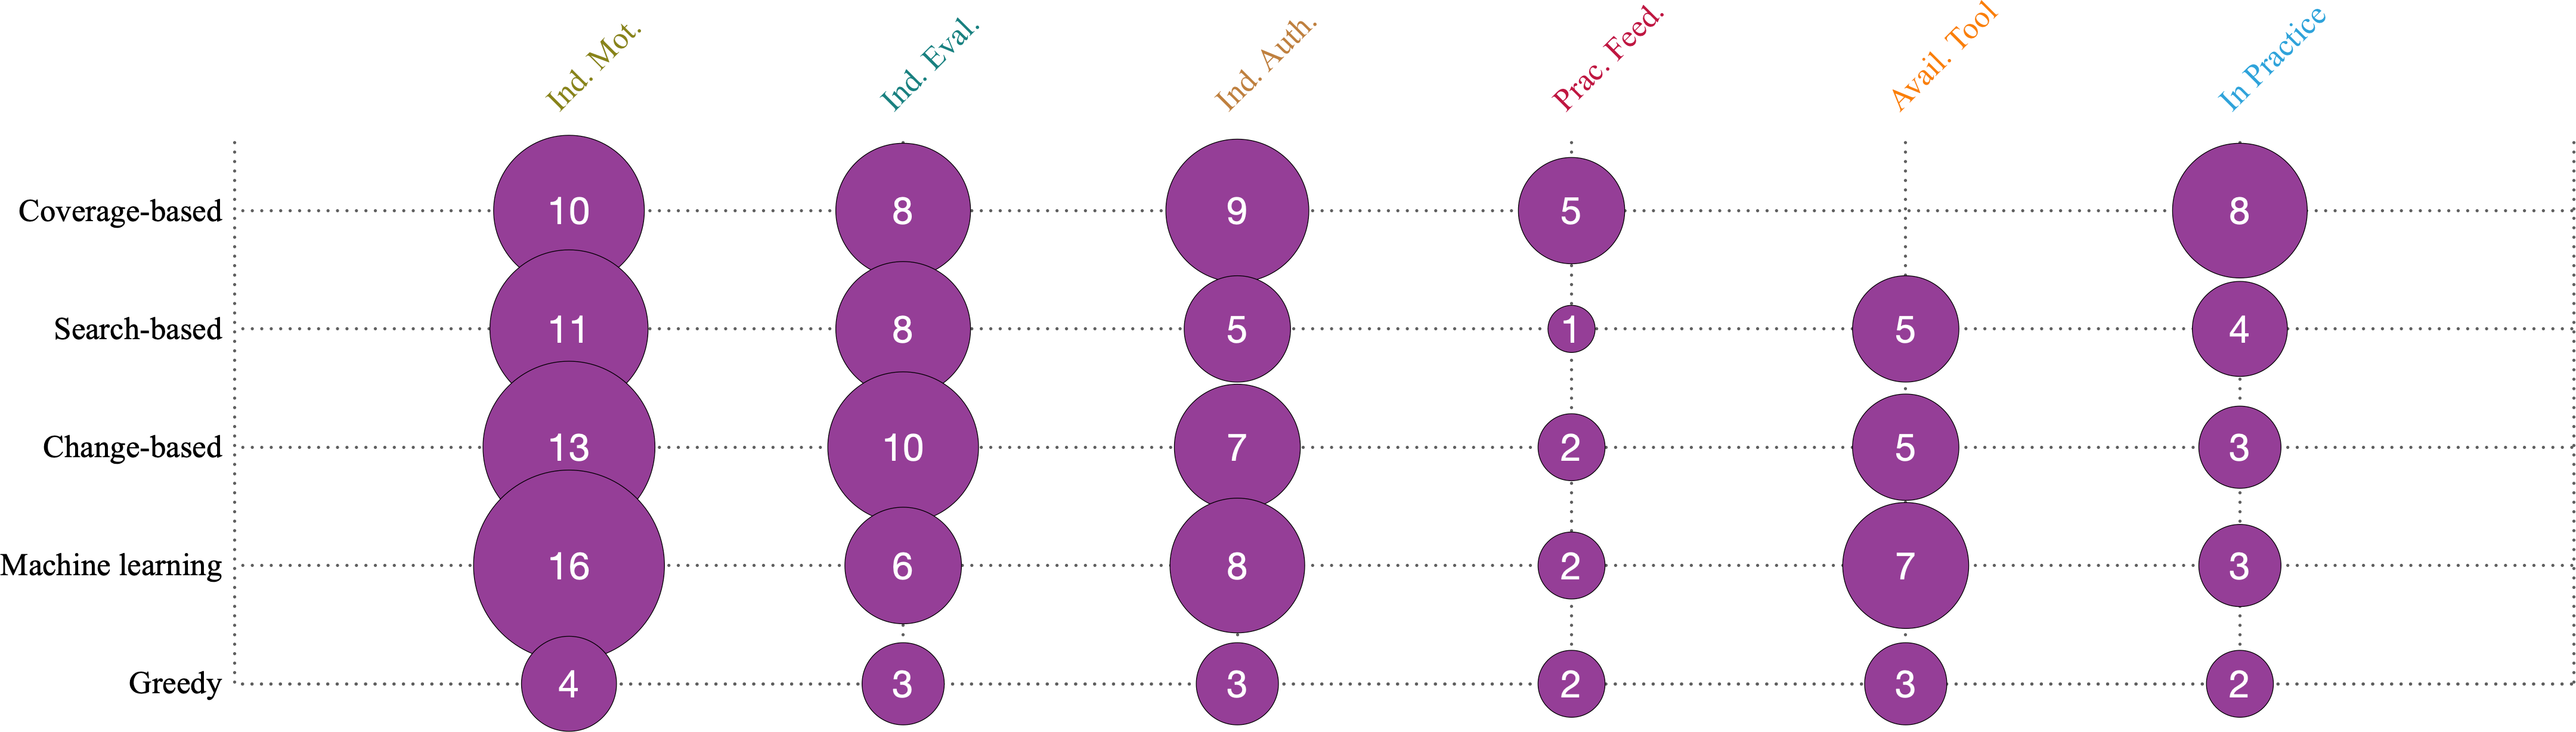
\includegraphics[width=\linewidth]{approaches_applicability.png}
%  \caption{Mapping of approaches and techniques that have seen practical application on at least 2 papers.}
%  \label{fig:approaches_applicability}
%\end{figure}

\autoref{fig:approaches_applicability} shows the relationship between the applicability criteria and the approaches that have seen real-world usage.
The figure shows approaches with at least two papers put into practice\footnote{Constraint-based, graph-based, similarity-based, trace-based, manual classification, cost-aware and history-based approaches have one paper each implemented in practice.}.
Unsurprisingly, the most common information-type and algorithm-type approaches are the ones that see the most real-world usage.
Coverage-based approaches dominate the implementations of techniques, despite previous concerns regarding the cost of measuring coverage \cite{herzigkeynote}; although time-consuming, coverage measurements are easy to obtain in most programming languages.
Conversely, there are 16 papers proposing machine learning approaches, but only three were implemented, likely because machine learning models are only as good as the data they are fed; often, obtaining data of enough volume and quality is more difficult than implementing the method itself.

From the practitioners' point of view, one possible source of information is grey literature --- that is, material produced by experts and published without peer-review.
However, this data is decentralized and unstructured, making it difficult to locate useful information.
We did find one example: Netflix has a post on their blog \cite{netflixlerner} describing a system they developed inspired by \citetalias{spieker_reinforcement_2017}.
This indicates that grey literature might be worthy of investigation, but such an effort would fall beyond the scope of the current study.

To provide some insight into the state of practice, we surveyed 23 practitioners who are involved with software development and/or testing at their workplace.
60\% of respondents claim they do not know about \rt tools that originated from research, which corroborates the well-known lack of communication.
35\% say they use or have used a tool to aid \rt; however most of these claim the tool was developed specifically for their needs, so it is not clear that their origins can be traced back to Software Engineering research.


\begin{tcolorbox}%[size=fbox]
%\small
\textbf{Summary of RQ3.} From the papers and the responses we received, we have evidence that 20 papers propose techniques that are still being used in practice.
It is a relatively small number, but it shows that \rt research can have concrete positive impact on real-world software development.
Unfortunately, many of the techniques that are implemented fall out of use after some time, as an ongoing effort is needed to motivate their usage and keep the tool relevant and updated.
There is a hint of evidence stemming from grey literature, although practitioners themselves, when surveyed, mostly claim to be unaware of \rt techniques originated in academia.
\end{tcolorbox}

%----------------------------------------------------------------------------------------
%	Test Suite Orchestration
%----------------------------------------------------------------------------------------
\chapter{Test Suite Orchestration}\label{chap:orchestration}
\lhead{\emph{Test Suite Orchestration}} % Set the left side page header to "Introduction"
%----------------------------------------------------------------------------------------
%	Insights from Industry
%----------------------------------------------------------------------------------------
\chapter{Insights from Industry}\label{chap:industry}
\lhead{\emph{Insights from Industry}} % Set the left side page header to "Introduction"

\section{Summary}\label{sec:ind_summary}

It is well-known that not many ideas proposed in academia make their way into practical usage.

Recently, there has been research specifically about the ``Industry-academia gap''.

In this paper, we aim to bring more light into this topic by drawing some comparisons between points frequently discussed in the literature and the actual state of practice in an industrial partner.

Section \ref{sec:background} gives some background on regression testing. Section \ref{sec:rqs} contains the research questions and their discussions. Section \ref{sec:related} highlights relevant related work. Section \ref{sec:threats} points potential threats to the validity of this study. Finally, \ref{sec:conclusion} offers our closing thoughts.


\section{Research Questions}
\label{sec:ind_rqs}

The following research questions represent the main objectives of the collaborative interaction with the industrial partner.
Generally, the contribution of this period is the identification and explanation of notable challenges involved with industry-academia collaboration and the advancement of practical software testing techniques.

Keep in mind these are not the questions asked directly to the practitioners (these are found in \Cref{app:surveys}), but they were used a starting point to design the interviews.

\paragraph{RQ\ref{chap:industry}.1. What are the issues most frequently noted by software testing practitioners?} --- We want to hear from the practitioners themselves what are the testing challenges they face on a daily basis.
It is important to understand whether these challenges are the same that motivate software testing research, or if there are concerns from industry that are yet unaddressed by researchers.

\paragraph{RQ\ref{chap:industry}.2. What are the challenges that arise when trying to incorporate academic insight in practice?} --- Based on their previous experiences with software testing techniques, we would like to know what worked and what didn't, and for what reasons.
We know beforehand that it is not trivial to convert academic knowledge and insights into a company environment, but we should understand with more details why this conversion is so difficult to accomplish.

\paragraph{RQ\ref{chap:industry}.3. What are potential paths to improve collaboration between academics and practitioners?} --- With this we seek to capture what the practitioners are looking for when they are approached by academics.
This discussion should help researchers propose more relevant collaborative projects, as well as set the expectations of practitioners as to what is feasible to achieve when working together with academics.


%\todo{Note: The RQs are 5.x because this is chapter 5 of the thesis, it appears as ch.1 because I've omitted the others}
%How can academics make their work more accessible for interested practitioners?


\section{Overview of Testing at Ericsson}\label{sec:ind_overview}

Regression testing is a topic that has been extensively studied for decades.

It includes topics such as \textit{test case selection}, \textit{test case prioritization} and \textit{test suite reduction}.



\subsection{Regression Testing in the Literature}

Most academic studies are focused on unit tests or lower-level integration tests.

\subsection{Regression Testing at Ericsson}

In the mid-2000s there was a shift to agile development which affected the testing workflow.

Ericsson employs a ``test strategy pyramid'' that starts with unit tests at the lower end and goes up to network tests at the high end.

A substantial part of the testing cost comes from the high-level network tests, which are complex and expensive, as they involve multiple layers of software as well as physical and simulated hardware.

There is a ``shift left'' objective that aims to bring fault-finding into lower levels of the pyramid.

There are frequently executed ``checks'' (that may employ some sort of test case selection) and overnight ``tests''.

When an overnight test fails, it is often due to test flakiness or environment misconfiguration. Often it is not an error in the SUT proper.

In the integration/multi-component level, it is often the case that higher-level/more complex tests cover lower-level/simpler functionality by definition. However, there is no system in place to refactor and remove older tests that are no longer necessary.


\section{Interviews}
\label{sec:ind_interviews}


Information about how testing is performed at the industrial partner and regarding the challenges still faced at the company was gathered via a series of interviews.
This was initially in the form of unstructured conversation, while the interviewer understood the central details.
After the basics were covered, we performed a series of 30- to 60-minute sessions with 1 to 3 people at a time asking more focused questions.

\Cref{table:interviewees} lists the roles of the interviewees, who are anonymized for this study.

\begin{table}[]
\centering
%\scriptsize
\rowcolors{1}{}{gray!10}
%\setlength{\tabcolsep}{6pt}
\begin{tabular}{ll}
\toprule
\textbf{ID} & \textbf{Role} \\
\midrule
R1 & Functional Area Domain Tester \\
R2 & Functional Area Domain Tester \\
R3 & Functional Area Domain Tester \\
R4 & Continuous Integration Test Manager \\
R5 & Module Test Manager \\
R6 & Module Test Manager \\
R7 & Senior Test Specialist \\
R8 & Senior Test Specialist \\
\bottomrule
\end{tabular}\\
\caption{Team members interviewed for this study.}
\label{table:interviewees}
\end{table}

%\todo{List of acronyms is here to help with writing/reading the chapter in isolation; later this will be moved to the appropriate page.}
%
%Acronyms:
%\begin{itemize}
%	\item MCT: multi-component testing
%	\item SDC: source delivery check
%	\item SBT: source baseline check
%	\item XFT: cross-functional team
%	\item CI/CD: continuous integration/delivery
%	\item TR: trouble report
%	\item FOSS: free and open-source software
%	\item FAD: functional area domain
%\end{itemize}

\subsection{Roles and experience}

R1, R2 and R3 are members of the Functional Area Domain team\footnote{These team members were interviewed jointly; others interviews were one-on-one sessions.}.
They describe themselves as \quoter{the owners of the test suite}{R2} and are responsible for \quoter{monitoring the test results}{R2}.
In particular, they \quoter{are monitoring the nightly runs}{R1}, i.e. the LIRT or non-blocking tests.

R4, R5 and R6 are test managers, albeit R4 has a different responsibility.
The module test managers, R5 and R6, are responsible for the testing of particular modules, meaning \quoter{not working on specific features}{R5}.
\quoter{I also guide the teams on how to write test cases [...], how we organize test suites and so on}{R6}.
Meanwhile, the CI Test Manager R4 is \quoter{responsible for the machines and environment and some of the test framework parts. To simplify, we are doing the framework, the developers are writing the tests, the managers are designing the strategy}{R4}.

Finally, R7 and R8 are designated as test specialists, meaning they handle longer-term strategy.
\quoter{I work a lot with test strategies. How we should test features and products [...] from now until 2025}{R7}.
Despite the similar titles, there is a key difference between the two specialists: R7 is responsible for a long-term strategy of a specific core of products, while R8 has an overview of the entire company, so their job also includes sharing technologies and strategies among distant teams.

Aside from R8, who has a PhD on the topic of software testing, most of the interviewees did not have testing as a focus of their education while at university.
When asked about their education, R4, R5 and R6 are computer scientists and/or engineers, and most of the testing knowledge they had prior to working at the company was \quoter{standard university [curriculum], which contains tests}{R5}.
Meanwhile, R7 \quotes{graduated in media and communication}, so testing was \quotes{not covered in university}.
R4, R5 and R7 mention having a certification by the ISQTB\footnote{International Software Testing Qualifications Board}.
Additionally, R4 also mentions taking testing courses led by R8 internally, while R5 reports having attended workshops from \quoter{people [from the main office] presenting how testing should be done, but it was so high level that I couldn't understand how to apply it to my level}{R5}.
It is unclear if the testing courses/workshops mentioned by R4 and R5 are the same.

\subsection{Current practices}

Regarding the current testing practices, we want to understand what are the day-to-day activities performed by the team.
We would also like to know if there are any implementations of the regression testing techniques classically studied in research (selection, prioritization, reduction, amplification).

The interviewed team members are mostly working on MCT and have all mentioned two key processes for this layer: \quoter{[one] for delivery, [another] for less frequent runs}{R1}.
As previously discussed, we use the acronym SIRT to refer to a short execution of the test suite that happens whenever a developer pushes changes to be merged into the main branch of a module.
Due to time and resource constraints, \quoter{for [SIRT] there is selection, in nightly we run everything}{R1}.
This is also called the ``gating loop'', since a failing test prevents the change from being merged.
At the time of the interviews, \quoter{it's manually decided what goes in [SIRT]}{R6} and \quoter{the running time [...] for MCT is 15-20 mins}{R5}.
The LIRT is also known as ``assessment loop'', which includes all tests in the suite, and can take up to 10 hours.
As a general rule, the tests in SIRT are a subset of the LIRT suite.

\paragraph{Selection.} In MCT, it is manually determined whether a test should be included in the SIRT. As an example, \quoter{yesterday, we got the question, `should we include this in gating?' I don't know, I just go by feeling. We have to see if the feature seems fundamental or important somehow}{R5}.
Despite this practice, most of the interviewees are aware that there could be a better way of doing things: \quoter{I think there should be more strategy than just me thinking}{R5}.
When this finding was reported to R8, who oversees testing all over the company and does not work with R1-7 on a daily basis, they mentioned that the company does have an internal tool for test selection and was surprised to find out this team did not use it.
R4 explains: \quotes{we had attempts to integrate [the test tool mentioned by R8] but it did not work out so well. I think we never built a business case for [the new version of the system] and it ended up way in the backlog. In 2017 or 2018 we said `this is something we should add to our plan', but we did not do anything.} 
However, \quoter{it might be deployed in other parts of the company}{R7}.
That said, R8 questioned the necessity of \tcs in a well-designed agile production: \quoter{why do you need to select? The agile principle says we should test everything}{R8}.

\paragraph{Prioritization.} This does not appear to be an active concern for the team and there are no techniques in place for advanced prioritization: \quoter{for prioritization, nothing specific}{R1}.
\quoter{We have suites, which are groups, e.g. for sub-modules, gating or not. Then I think it's just the order they're written.}{R5}.
However, \quoter{now we have introduced shuffling for the assessment}{R5}, i.e. random ordering of the test cases.
The motivation for this is not decreasing the feedback time, but rather \quoter{to help find problems with unstable tests}{R1}, which might be flaky according to the execution order.
R8 again expressed a concern: \quoter{using the same TCP approach every time, wouldn't the same test be top priority every time?}{R8}.

\paragraph{Reduction and Amplification.} These techniques are absent in the workflow. \quoter{We don't have any tools that helps us in any way in shrinking or expanding the tests}{R5}. \quoter{No, we don't have anything like that}{R6}.
Regarding reduction, \quoter{if it happens that there are too many tests for overnight, there would be an initiative to reduce}{R1}, but \quoter{we can put more machines and we can run more}{R6}.
Interviewees generally agree that it is more cost-efficient to increase computing capacity of testing servers than to spend human time determining which tests to remove.
For amplification, there appears to be no interest in automating the process.
There is a protocol, however, to manually augment the test suite in the situations where a fault slips through a layer of testing: \quoter{if a fault was found later in test or in the field, we try to investigate why did it slip through, and we should have a test for that}{R1}; then, \quoter{after the fact, if there is time, we can go back and understand why a needed test was not in the plan}{R2}.

\subsection{Common issues with regression testing}

Part of the questions asked interviewees to detail the common issues they notice with the current state of the test suite and the testing practices at their team.
They were asked to elaborate on five key points: fault detection, flaky tests, running time, increasing test scope and reducing test scope.

\paragraph{Fault detection.} Most respondents have reasonable confidence on the fault detection capability of the test suite, although several admit that they might not have the data needed to be sure and it mostly relies on the fact that few faults are detected in the delivered product.
Since most of the monitoring of the test suite happens within the CI/CD pipeline, there is an understanding that most of the fault detection actually happens before that, on the developers' local environments.
\quoter{Perhaps a suite is going green always, but it's being used by a developer while they are writing}{R5}; \quoter{the very good test cases [...] find faults when running locally at the developer's computer}{R1}.
\quoter{[Developers] are quite happy doing MCT testing locally. I think they find a lot of bugs there. They rely on SIRT to feel confident they won't break everything when delivering}{R2}.
Thus, most of the faults detected during the SIRT would be a result of conflicts between changes merged by two developers asynchronously, rather than the result of poor code submitted by a single developer.
That said, the team recognizes that the current version of the test suite is not 100\% effective in avoiding faults or ``slips'' (when a failure is detected in a higher layer of testing than it should have been), especially during the gating loop.
\quoter{We can't have all the test scope in the gating loop. There is a discussion of having specific test cases for gating in order to have more coverage, instead of just a subset}{R6}.
There is a back-and-forth discussion between two sides of the team: one wants the gating loops to pass more often and let the changes through, the other wants them to be stricter.
\quoter{The flow guys remove everything to get the flow going, but we are like I don't know, this test might be important}{R5}.
Once a fault slips and it is detected at a later testing phase or in the field, there is \quoter{a systematic way of processing trouble reports (TRs) and we can identify where it is needed to add tests}{R5}.
Regarding that, R8 brings an analogy: \quotes{if you only take care of the shootings, you do not solve crime}, implying that the above is not an effective strategy for delivering a fault-free product.

\paragraph{Flaky tests.} Although techniques for addressing flaky tests falls beyond the scope of this thesis, it was a topic brought up frequently during the discussions --- \quoter{that's the worst, we have a lot of those}{R5} --- it is strongly related to the above point regarding fault detection.
\quoter{The tests are run distributed in several computers connected to a network, so when the load gets really high, running thousands of tests at night, we can get different behavior compared to running the tests manually}{R2}.
To account for this, \quoter{we started shuffling the order of the tests}{R3}, although sometimes the developer who wrote the test case admits \quoter{'I don't know why it fails if it comes later in the suite'}{R3}.
There is an agreement that \quoter{creating stable [non-flaky] tests is cumbersome}{R1} and, \quoter{if it's due to the code, it's usually timing issues}{R2}.
Some team members believe this could be relieved with better test design: \quoter{most of the times, flaky tests are caused by poor testing}{R8}; \quoter{a lot of people develop tests but are not very familiar [with test design principles]}{R1}.
In fact, upon investigation, testers in the functional team \quoter{find more problems with the tests than with the products}{R1}.
The test managers share this perspective: one says \quoter{less than 50\% of our failures are actually a product fault}{R6}, while another thinks \quoter{it's 30/30/30 [actual error/test design/environment issues]}{R5}.
Despite being aware of this, the team has learned to deal with the issue.
For example, \quoter{we have one test that is mostly working, but it's failing once a week}{R1}.
At first glance, it might appear that this test is not adding value to the suite, but actually, \quoter{we can double and triple check that it's not actually a bug in the product}{R2} and, \quoter{if it starts failing every day, we would look into it, so there is some value}{R1}.
Due to situations like this, \quoter{every day there's at least one failure}{R6} in LIRT runs, but the team recognizes the troublesome tests.
That's not to say these tests are ignored: \quoter{usually, we are currently working on a solution but it's not done yet}{R2}.
Since these tests are particularly difficult to fix and they still provide some value to the test results, they are left as-is unless a fault related to it slips to another layer of testing.

\paragraph{Running time.} Test managers claim that \quoter{the running time is fairly okay, [...] for MCT 15-20 mins}{R5}.
More important than the running time itself (which is offloaded to virtualized testing server) is the queueing time, which increases during the day as more test jobs are dispatched to the servers by the developers. 
For this, \quoter{we can also test in parallel a lot of things [...] and spin up more virtual machines as needed}{R5}.
Naturally, \quoter{the main pain point is the gating loop, since we want to have shorter feedback, it's more loaded during the day as people are working and at night it's mostly free}{R6}.
The parallelization is limited, however, at least in some layers of testing.
Since the main branch of a module is updated linearly, separate commits cannot simply be tested in parallel and then merged without being tested together, so what may happen is that a certain number of commits is tested in parallel and, if the tests of at least one passes without issue, only one is merged into the branch.
Failing tests are sent back to the developer, and other passing commits are queued for execution again, using the newly-updated branch as the base.

\paragraph{Increasing test scope.} Although simply increasing the number and even coverage of tests is not a challenge on its own, doing so maintaining quality and consistency might be.
Currently, \quoter{it's the feature developers who write tests}{R6} or, in other words, developers mostly write tests to cover their own code.
\quoter{The problem is that cross-functional teams (XFTs) are racing for product delivery}{R6} but, since many developers are not necessarily proficient in good test design, \quoter{it's easier to copy paste code. Tests are not always great. I would say it's something we need to work on.}{R6}.
As the product itself grows in scope, \quoter{it makes sense that the tests increase at the same rate, but to me we are not increasing the test scope at fast as the product}{R7}, so there is still a feeling that the tests are seen as secondary compared to the product itself.


\paragraph{Reducing test scope.} Many interviewees agree that this is a difficult challenge that is not currently well addressed.
\quoter{Cleaning and updating old tests is most difficult}{R1}, but \quoter{who can decide if a test case should be removed?}{R5}.
Even if refactoring or reducing the test suite is discussed, \quoter{it's cheaper to leave [the test] there and run it than spend money to have people looking at it}{R5}, especially in LIRT.
On the more restrictive \quoter{SIRT, if new tests are coming in, we have to shift out legacy tests}{R6}, so in this situation the tightening of test scope is essential.
Although this perspective has changed over time: \quoter{in the beginning of [the new version of the system], we said `everything should be gating', but now we have too many test cases}{R6}.
Often, a test \quoter{might make sense when it's first written, but many developers go into the same same suite, so over time it might degenerate a bit}{R7}, which would call for refactoring if not outright removal.
The specialists bring a complementary insight: \quoter{even if tests are obsolete in terms of fault detection, they might still be useful for root causing}{R8}, meaning that a test that doesn't find faults might help narrow down the causes why other tests are failing.

\paragraph{Testing costs.}
Testing costs is often discussed in the literature when it comes to the applicability of solutions, but it is not a major concern to most of the interviewees.
The team uses cloud-based testing, and \quoter{the cloud infrastructure is completely ours}{R4}, not outsourced to other companies.
The functional testers \quoter{don't know [the cost]}{R1}, but it is \quoter{probably a lot}{R2}.
R6 also says \quotes{I don't know how much kilowatts it's drawing}, but, according to R5, \quotes{I don't think it's more expensive than watching a youtube video}.
It's understood by several team members that resources can be increased if required, and one manager goes on to ask \quoter{why not run everything more and faster, instead of selecting things? It might not be cheaper, but it seems like the company is more willing to pay for equipment than employees}{R5}.
When asked specifically who would know this, the answer is \quoter{the area product owner}{R4}, who \quoter{handles the budget with inputs from us, according to how much we use and how much we'll need}{R4}.
The specialists highlight that \quoter{earlier test loops are much cheaper}{R7}, so it is important to detect faults as early as possible.
Furthermore, even if \quoter{electricity is so cheap}{R2}, \quoter{we have some hardware that is super expensive, it costs as much as house}{R7}.
For this reason, \quoter{we want to make sure the test cases that execute on that hardware are only the most important ones}{R7} and this type of load balancing is still being worked on by the cloud infrastructure team.


\subsection{Collaboration with Academia}

Another point relevant to this study is the practitioners' current relationship with academia.
Firstly, they were asked if they keep themselves informed about recent research trends in software engineering.
Most respondents answered in the lines of no, \quoter{I don't find the time or I don't prioritize it}{R1}, \quoter{our level, we don't really have time}{R5}. 
R2 occasionally reads books on the topic, although these are more practical in nature rather than research works.
Time is the main issue, because \quoter{because the research world is huge and there's so much happening}{R7}.
R5 thinks \quotes{it would be interesting to see how other big companies do it}, which alludes to initiatives such as the Google Journal Club \cite{googlejournal} that have seen success in some companies but does not appear to be a practice in this case.
\quoter{I suppose someone at the company has this assignment somewhere}{R5} and, indeed, this someone is likely R8: \quotes{I read the literature and try to apply it}.
However, \quoter{academia is both ahead and behind [the state of practice]. It's ahead because it's looking into techniques that might be useful many years from now. It's behind because it doesn't keep up with the current challenges in the state of practice}{R8}.
There is a perception that academic work is important, but ultimately disparate from the immediate needs of practitioners.

A follow-up question asked if the team member were aware of any current tool or practice at the company that had origins in academic research.
The general response to this was uncertain.
Nobody could point to a specific and concrete example, but there are some possibilities, for example \quoter{before we used to run everything manually, then this scheduler was developed that can define when and what to run}{R5}, but \quoter{I don't know if that's from academia}{R5}.
Furthermore, \quoter{over the years we have had much cooperation with research, so I would assume there is something}{R7}, but again no clear example was given.

When asked if they still keep in touch with a friend or colleague in the academic world, it appears this is not common.
\quoter{We always have old colleagues that are PhD, but unfortunately we don't hang out so much}{R5}, and \quoter{I think all my friends from college are now in industry}{R4}.

Continuing on this line of thought, some respondents mention there is some collaborative projects that happen involving the company and a nearby university.
\quoter{At least in [this city], we have been keeping a close relationship with the university}{R4}, although the main objective is not necessarily to develop new research or technology, but rather \quoter{to vacuum the competencies from the university towards us}{R4}.
This mostly occurs through co-sponsorship of Master degree students: \quoter{we announce some thesis work and try to keep them here}{R4}.
R7, however, mentions volunteering \quotes{a study by another company [about] roles for testers, [...] I think [the researcher] is employed by both that company and the local university}, indicating there is some cooperation happening between the two companies and the local university.
R1, R2, R3 and R6 provide a negative answer: \quoter{no, there hasn't [been collaboration] from what I know}{R6}.
Regarding specifically an experience similar to the present work, e.g. a visiting researcher collecting data and performing a study on the current practices of the company, \quoter{no, I think you're the first PhD I'm having contact with}{R7}.

When asked what would motivate the team to incorporate a technique from academia into their workflow, the main factor is the ease of use and the resulting reduction of workload from the team: \quoter{how easy to implement is it? Does it remove manual work?}{R6}.
However, regarding risks and challenges of doing so, there are several relevant points.
A major one is the matter of security.
It is recognized that \quoter{external tools can be security risks}{R8} especially because \quoter{we don't know if the researchers are rigorous with their implementation}{R8}; indeed, it appears that \quoter{something happened some years ago and, for security reasons, we don't want to incorporate open-source tools into the process without making sure what they are}{R5}.
Due to this, \quoter{we have this [free and open-source software] (FOSS) process. If you want to use open-source you need to submit a ticket, then it needs to be scanned and approved}{R5}.
Furthermore, it is hardly the case that general open-source tools can be incorporated without bespoke modifications: \quoter{it usually doesn't fit}{R8}.
For example, \quoter{researchers might assume a certain level of quality or standardization among test cases, but in reality test design is often bad}{R8}, which could explain in part the existing gap between academic experiments and real-world usage.
In addition, \quoter{we have to figure out how to feed data to the tool}{R2}, which is not always trivial: \quoter{the algorithms are usually fine, but it's hard to provide the data that is asked for}{R7}.
One possible reason for this lack of data is that many of the test executions are triggered by the developers themselves while they are still working on a new feature or bug fix. 
A failure at this point might be a legitimate detection of an error, or it might be expected by the developer who triggered the test while being aware that the code was unfinished; it is difficult to filter out this type of data and provide a ``clean'' input to an algorithm.

Despite the above concerns, the team members expressed a drive to make changes to their workflow and say that \quoter{we are quite good at solving technical difficulties}{R2} and performing the necessary modifications and experiments is not the main obstacle to overcome.
Rather, \quoter{the big problem is that there are unclear responsibilities}{R1}, so \quoter{It's not clear who we would need to convince to make changes to the process}{R1}.
This opinion is corroborated by other team members: \quoter{I always see bureaucracy as a part of the difficulty of getting things done}{R5}; \quoter{I think the main challenge would be convincing people to spend time and money on it}{R6}; \quoter{the problem [...] is to find out who is going to pay for it}{R4}.
Considering the scale the company, however, \quoter{I think it's good we have this organization, the company is really big so we need structure, but it can make it harder to make these smaller changes}{R4}, but it is clear that \quoter{programs are measured by how many features they are developing, especially in the customer end. You're measured more on feature throughput than product care}{R4}, so software quality activities such as testing and refactoring, which are ``invisible'' to the customer, are hard to prioritize.
R7 mentions a dedicated internal group \quoter{who can work with anyone within the company}{R7}.
Together, they performed a study to improve test case selection in their next-generation products, but it is \quoter{challenge to convince someone to do it}{R7}.
\quoter{The project [with the internal group] was a theoretical experiment, but we did not try it in practice. There's a limited budget to how many improvements we can do in parallel and other things were prioritized}{R7}.

\subsection{Metrics}

In conversations with R4, the topic of metrics for measuring test suite effectiveness was discussed.
Metrics familiar to researchers, such as APFD, is not part of the common language at the company, but there is a current initiative to add some measurements to the testing flow and extract useful metrics from them.
Specifically, three metrics, all under consideration but not in active use, were explained:

\paragraph{Product Fault Finding Capability (PFFC).}
The objective of this metric is to determine whether faults are being detected in the ``correct'' layer of testing, or if they are slipping to more complex and costly testing.
It is measured by two variables: (1) the number of \textit{new product faults found} ($npff$), which counts the number of new faults after a test execution and analysis of failures, and (2) the number of \textit{slips} ($slips$), which is the number of faults detected in a certain layer of testing that, upon inspection, should have been found earlier in the testing stack.

$$ PFFC = \frac{npff}{npff + slips} $$

\paragraph{Cost to Fault Ratio (C).}
It is particularly difficult to measure the cost of an individual test, but it should be possible to at least estimate the cost of an entire test suite, or the cost of each detected fault.
This metric does that by multiplying the \textit{machine costs} ($MC_n$) with the number or sizes of \textit{system test plans} ($STP_n$) meant for execution in that machine.
The resulting value is then divided by the number of detected faults in order to get the cost per fault.
Ideally, this should ensure only critical tests are executed in the most costly testing servers.

$$ C = \frac{MC_1 \times STP_1 + MC_2 \times STP_2 + ... + MC_n \times STP_n}{faults\ detected} $$

The obvious flaw with this metric is that it might disfavor products with a low number of faults --- as fewer faults are detected, the cost per fault ratio will greatly increase.

\paragraph{Reliability (R).}
This metric targets specifically flaky tests, providing a value to their reliability.
It is simply a division of the number of \textit{faults detected} ($fd$) by the test suite by the number of \textit{failed runs} ($fr$) of that same suite.

$$ R = \frac{fd}{fr} $$

Suites with low reliability are ones that fail often, but rarely lead to a true detection of errors in the SUT.

\section{Challenges Identified}\label{sec:ind_challenges}

%----------------------------------------------------------------------------------------
%	The Industry-Academia Knowledge Gap
%----------------------------------------------------------------------------------------
\chapter{Challenges Between Industry and Academia}\label{chap:gap}
\lhead{\emph{\nameref{chap:gap}}}

\todo{Is there a better title for this?}

While the review in \Cref{chap:literature_review} indicates that \rea is a growing concern among \rt researchers, it's still only being addressed with any depth on a minority of secondary studies.
It is clear that several authors believe \rea is a challenge worth addressing in research, but there is not a lot of available \rt literature focusing on the steps that need to be taken in order to improve academia-industry communication and shorten the technology transfer gap.

We conclude this work by highlighting some key challenges that we have identified, combining data found in the literature itself, in the authors' responses and in the practitioner survey.
These are challenges that may have been addressed in certain circumstances but remain unsolved in a broad sense, as they are still present in several recent works.
Along with each challenge, we make some suggestions that could be applied by Software Engineering researchers and/or Software Testing practitioners — these could be actionable steps for upcoming primary studies, or further avenues of investigation for secondary or meta studies.
\Cref{table:challenges} provides the summary of the challenges we identified, indicating the primary source of our observation (i.e. the literature, the authors and/or the practitioners).

\begin{table}[]
\centering
\scriptsize
\rowcolors{1}{}{gray!10}
%\setlength{\tabcolsep}{6pt}
\begin{tabular}{llllll|llllll}
\toprule
\textbf{ID} & \textbf{Title} & \textbf{L}  & \textbf{A} & \textbf{P} & \textbf{I} &
\textbf{ID} & \textbf{Title} & \textbf{L}  & \textbf{A} & \textbf{P} & \textbf{I}\\
\midrule
CH1 & Alignment of motivations             &   				&  			     & \fullcirc      & \fullcirc &
CH6 & Absence of TSR/TSA                   & \fullcirc 		&                & \fullcirc 	  & \fullcirc \\

CH2 & Realistic experimentation            & \fullcirc 		&                &                & &
CH7 & Clarity of target                    & \fullcirc 		&                &        	      & \\

CH3 & Scalability                          & \fullcirc 		&                &                & &
CH8 & Skepticism                           &                & 	 & 	  & \fullcirc \\

CH4 & Relevance of metrics                 & \fullcirc 		& \fullcirc 	 &                & &
CH9 & Data quality/availability        &                & 	 & 	  & \fullcirc \\

CH5 & Developing usable tools			   &            	& \fullcirc 	 & \fullcirc      & \fullcirc &
CH10 & Communication                       &                & \fullcirc 	 & \fullcirc 	  & \fullcirc \\
\bottomrule
\end{tabular}\\
\begin{flushleft}
\scriptsize Source(s): \textbf{L}: Literature; \textbf{A}: Author questionnaire; \textbf{P}: Practitioner survey; \textbf{I}: Industry partner.
\end{flushleft}
\caption{Summary of main challenges identified by this study.}
\label{table:challenges}
\end{table}

% ===================

\paragraph{CH1: Alignment of motivations}
When asked what would convince them to implement and use an~\rt tool, eight surveyed practitioners gave responses that can be synthesized into ``\textit{it would make my work easier}''.
This general sentiment matches the responses received during interviews at our industrial partner.

There exists a mismatch between academic motivations and industrial needs: research is concerned with discovering novel techniques that might provide marginal effectiveness gains over the state-of-the-art, while practitioners are mostly concerned with any solution that simplifies their workflow.
In other words, even if an \rt technique has the potential to greatly reduce the testing time of a suite, practitioners will weigh those benefits against the effort required to implement the technique and adapt/maintain it for their needs.
This is not to say that the current research motivations are ill-informed: it is the role of academia to push the boundaries of what is possible in theory first, and sometimes this theory takes many years to find relevance in practice.
One interviewee from \Cref{chap:industry} gave an example of this: \quoter{mutation testing\footnote{Mutation testing refers to a set of techniques that introduce artificial errors in the \sut in order to validate the efficacy of a test suite \cite{somethingsomethingmutation}.} has been in the literature since the 1990s, and it is starting to see adoption in industry today}{R8}.

If the researchers have the objective of implementing their approach, they must be certain that it is addressing the current needs of practitioners.
An obvious way to achieve this, which is also confirmed by our literature review, is by developing techniques through direct partnerships between academic researchers and industrial practitioners (or even open-source communities).
In these cases, the practitioners bring realistic examples of the challenges they face and, as a result, these collaborative works tend to produce results suitable for practical applications and could serve as a guideline for other, purely academic, approaches.

Naturally, not all research can be done with industrial partnerships, and in these cases there is difficulty in finding what exactly is relevant to current practitioners.
One possible source of this information is grey literature: information produced by experts in a field, but without necessarily following academic guidelines, in the form of blog posts, videos, magazine articles, talks etc.
Practitioners who produce grey literature can help inform researchers about the current state of practice, the main existing challenges in software development, and successful implementations of techniques (e.g. the aforementioned Netflix blog~\cite{netflixlerner} which details the process of bringing a technique from a paper into their workflow).

Ultimately, the unavoidable reality is that academics and practitioners work towards different goals.
Researchers are motivated and driven by publication; indeed, the point of research is to aggregate information into a body of knowledge that grows gradually over time.
Historically, academia does not encourage researchers to continue working on a project after the related paper is published and ``see it through'' to an eventual application of a technique.
In fact, the pursuit for novelty can diminish the perceived value of a researcher who is willing to perform experiments and do the additional work to implement a technique.

This is in direct contrast with the desires of industry.
Few companies are willing to commit time, money and human resources into developing novel techniques that may or may not provide value or savings in the long term.
Rather, they would rather adopt practices with a proven and predictable outcome.
%The space between novel and theoretically valid techniques and ones that ensure long-term value in practice is 

% ===================

\paragraph{CH2: Realistic experimentation}
It is clearly not possible for every research paper to feature practitioner co-authors or to rely on an industrial partnership for experimentations.
Selecting the right subject for experiments is a decisive point when writing a paper about a technique.
Older studies on \rt would often rely on the ``Siemens programs''~\cite{hutchins1994experiments}, which is believed to have caused an overfitting of results to a particular kind of software~\cite{do_recent_2016}.
More recently, the Software Infrastructure Repository (SIR)~\cite{do2005supporting} (e.g. \citepalias{schwartz_cost-effective_2016}) and Defects4J~\cite{just2014defects4j} (e.g. [\citetalias{noor_similarity-based_2016}, \citetalias{azizi_retest_2018}]) have been used to similar ends.
Having common subjects can provide replicability benefits when directly comparing techniques, although is not always clear if they approximate the difficulty of testing real software.
Authors who are able to collaborate directly with members of industry gain an enormous advantage if they are allowed to run experiments on production code, but it is also clear that not every paper will have that opportunity.

The most obvious alternative is to use large-scale open-source software (e.g. from the Mozilla \citepalias{zhou_beating_2020} and Apache 
[\citetalias{oqvist_extraction-based_2016}, 
\citetalias{bertolino_learning--rank_2020}, 
\citetalias{pan_dynamic_2020}, 
\citetalias{bagherzadeh_reinforcement_2022}, 
\citetalias{chen_context-aware_2021}]
 foundations) as subjects, since the communities developing these programs follow procedures much like the developers working for corporations .
This is also far from trivial.
The larger the software, the more time a researcher will need to dedicate in order to understand it and to adapt the technique to it, sacrificing the possibility of experimenting on a larger variety of subjects and thus again bringing the risk of overfitting.
Additionally, there is no established consensus regarding which properties an open-source program must satisfy in order to be a satisfactory subject.

Alleviating this issue would require effort from both researchers and practitioners.
For example, Google has an open dataset of testing results~\cite{googledataset}, and \citetalias{spieker_reinforcement_2017} combined it with one from ABB Robotics.
As a result, this combined dataset has already been used by other papers covering machine learning 
[\citetalias{wu_time_2019}, 
\citetalias{lima_multi-armed_2022}, 
\citetalias{pan_dynamic_2020}, 
\citetalias{sharif_deeporder_2021}, 
\citetalias{omri_learning_2022}].
Two practitioners mention that ``\textit{open source code/data is not provided}'' due to confidentiality reasons.
In those cases, our suggestion would be to provide some opaque information regarding the system, e.g. its programming language, the number of lines of code and/or tests, how many developers work on it, how frequently is the code updated, etc.
At the very least, this would help researchers choose subjects with similar characteristics.

% ===================

\paragraph{CH3: Scalability}
\rt techniques provide the most savings when applied to large-scale software projects, which can have multiple thousands of test cases.
Therefore, it is important that techniques are designed to scale up to any size of test suite, but few papers tackle this issue directly.
The trouble is that scalability is very hard to measure unless multiple subjects of different sizes are used.
One way to demonstrate scalability, beyond relying on industrial partners or large-scale open-source projects, is to artificially generate large datasets (e.g.~[\citetalias{miranda_fast_2018}, \citetalias{cruciani_scalable_2019}]), which are useful from the algorithmic perspective, but might not address other issues that arise in large-scale software development.
It is also worth mentioning that many \rt techniques can become \textit{disadvantageous} when applied to small test suites, as the cost of running the technique does not outweigh the savings in testing time.
So selecting the size of the experiment subject is important both to highlight the scalability of the tool in large software and also to consider whether the necessary overhead is a deal-breaker on small or medium projects.


% ===================
\paragraph{CH4: Relevance of metrics}
\Cref{sec:lit_rq1} shows that a wide variety of metrics has been used to evaluate the effectiveness of \rt techniques.
Some are used almost universally for a certain kind of challenge (e.g. APFD for \tcp), while others have nearly no presence beyond the paper that introduced them.

The abundant use of APFD and its variants indicate that, at least among researchers, there is a consensus of its utility and importance when evaluating \tcp approaches, although the usage of specific variants might hamper that benefit.
At the same time, it is not clear that a technique optimized for only APFD is sufficient to satisfy the needs of software developers in practice.
Still, APFD has been in use for over 20 years and it cannot simply be dismissed: at the very least it provides an agreed-upon method of directly comparing different techniques.

For the cases of \tcs and \tsr, there is less controversy on what are the most important metrics; reduction rate and fault detection loss appear to be the consensus among researchers, and there are fewer novel and single-use metrics.
As an example,~\citetalias{mehta_data-driven_2021} interviewed practitioners at Microsoft before deciding on their \tcs metrics, obtaining three main targets: reduction of cost, reduction of time and the failure detection rate.
We can observe in~\Cref{sec:rq1} that these concerns are reasonably addressed by \tcs techniques, although researchers still appear to prioritize reducing the selected set rather than ensuring all failures are detected.

The metrics of applicability and diagnosability \citepalias{correia_motsd_2019, zhou_beating_2020} are interesting propositions that consider other degrees of usefulness of a tool to developers.
Their existence indicates that some researchers still believe there is room for improved metrics that, perhaps, better map the requirements of real-world software, although these are rarely found in the literature.
Furthermore, ease-of-use is an important point to consider and, as far as we could detect, there is no established method of measuring it.

One practitioner stated: ``\textit{I don't think that academic tools are the best in a professional environment, I prefer commercial tools,}'' implying they believe academics are not measuring the results that matter most to them.
Indeed, managers allocating development funds will usually focus on the dollar savings a technique can bring, regardless of its theoretical effectiveness in fault-finding (as mentioned by respondent author \#43: \quotes{the cost associated with the 1\% bugs that were missed is too high}).

% ===================
\paragraph{CH5: Converting research into usable tools}
When techniques are designed in an academic context, they are normally developed as proof-of-concept works.
That is, the purpose is to show that the technique works and provides significant results according to some metrics.
However, this leads to two issues: either primary studies do not make their solution available for implementation, as we discussed in~\Cref{sec:lit_rq2}, or their experiments do not thoroughly consider practical concerns such as efficiency or the data requirements of a proposed approach.
Finally, what seems to matter the most is time and budget for developing a tool.
Papers are usually written targeting a hard deadline and their prototypes often do not see further work past publication.
It is inevitable that researchers will move on to new challenges, but their contribution would be amplified if the tool is, at the very least, open-source and well-documented so that other interested parties can continue the work in the future if desired.

If an \rt technique is implemented as a prototype that is shown to work on a certain kind of software, it is much easier to get the attention from a practitioner and convert the solution into something used in practice.
If feasible, an available prototype with solid documentation and usage instructions can be valuable both for study replicability and as a way to get developers interested in using it.
That said, the responsibility of developing fully functional tools should not fall solely upon researchers.
One practitioner stated that ``\textit{[\rt tools] need full security screening}'', and other said ``\textit{it requires an adaptation}''; these steps are not actionable by researchers in isolation.
As industry stands to benefit from scientific advances, it should be in its best interest to promote and fund the collaborations needed to continue development of promising prototypes.

This strongly relates to \textbf{CH1} regarding the motivations of academics and practitioners.
Even if a researcher has the desire to see a technique through to its applicability, or even just to provide a robust source code for the implementation of an approach, there is little incentive from the academic side for doing so.
Certain software engineering conferences have started to encourage or even require the inclusion of replication packages and source code of studies with an empirical component, which is a step in the right direction.

%\todo{Whose responsibility is it? A PhD student for example could work on this, but are there academic/publishing motivations for it?}

% ===================
\paragraph{CH6: Absence of \tsr/\tsa}
Out of \numpapers papers, only 8 are about \tsr and, surprisingly, only one covers \tsa 
 \citepalias{yoshida_fsx_2016}.
60\% of the surveyed practitioners claim that ``creating or updating tests'' is a major challenge in real-world \rt, so the desire for \tsa exists and there appears to be ample room for experimenting with new approaches and metrics.
However, most practitioners interviewed at the industry partner claim that increasing test scope is not a major concern, as even the manually-written tests can be too many.

On the other hand, they do mention the difficulty of refactoring and removing obsolete test cases as a frequent challenge, which aligns with 47\% of the surveyed practitioners.
\tsr could prove valuable to testers who need to manage ever-growing test suites and hardly find the time to manually assess tests that are obsolete or in need of refactoring.
In reality, this is often addressed by simply increasing the capacity of testing servers, but this is a costly and non-scalable solution.

This assessment of \tsr and \tsa techniques indicate an opportunity for researchers to develop novel methods for these challenges and to progress in directions that are in need of improvement in software development workflows.

% ===================
\paragraph{CH7: Clarity of target}
Several of the papers we reviewed don't clearly state key characteristics of their SUT, such as its programming language or its scale (either in lines of code or test cases).
For practitioners and other researchers to consider a paper worthy of investigation, it is important to know for which kind of system a piece of research was designed.

As mentioned in~\Cref{sec:lit_rq2}, few \rt techniques are language-agnostic and many do not inform the target language at all.
Similarly, the type of software (web, mobile, embedded, distributed, etc.) or its development paradigm are important factors to mention, seen in studies such as~\citetalias{zhong_testsage:_2019} for web services and~\citetalias{lima_multi-armed_2022} for software developed and delivered through continuous integration.
Not every tool can be used in any type of software, and it is likely that specific types of software might require specific solutions, so it is important to state the particularities of certain subject programs.
This is akin to the point of ``context factors'' brought up by~\citet{bin_ali_search_2019}, which helps to alleviate the issue by introducing a base taxonomy that can be used to categorize techniques.

Critically, there is often ambiguity on the very definition of test case.
Software testing can include unit tests, integration tests, multi-component tests, system tests, end-to-end tests and so forth.
Most papers do not make it explicit which layer of testing it is addressing. While it can sometimes be inferred with some domain knowledge, it is difficult to be certain for most readers.
This information would be valuable for interested practitioners and also for researchers who are looking to identify gaps in the literature.
On top of that, some papers use the term ``test case'' to refer to test methods, while others use it when referring to test classes/files (which contain several test methods), so the granularity of the technique is not always clear, and this can impact both effectiveness and efficiency analysis.
This challenge can be solved by having a paragraph dedicated to explicitly describing the properties and context factors of the experiment subjects.

% ===================
\paragraph{CH8: Skepticism}
In general, there is some degree of skepticism from practitioners regarding automated solutions.
For example, some interviewees at the industrial partner expressed concerns that a \tcs solution might leave out an important test, or that \tcp algorithms might always prioritize the same tests.
Their intuition is that performing selection (or even prioritization) manually allows for easier troubleshooting in case something goes wrong.
As for what can go wrong, the fear is to detect a fault later on, only to find out the test to detect it already existed, but was not selected or prioritized by the automated tool.

This calls back to a comment made by one of the responding authors in \Cref{sec:lit_rq2}: even if 99\% of faults are detected at a fraction of the testing costs, the remaining 1\% of slips is unnerving to the people responsible for the tests.
And even if a tool is shown to be safe, there is still a feeling that there \textit{might} be a slip that will only be revealed much later than it should have been.

Regarding \tsr, most developers are also opposed to outright removing tests, but are willing to put these tests in less-frequent rotations, e.g. weekly instead of daily.
Finally, for \tsa the practitioners are also doubtful that automatically generated or enhanced tests are as good as human-designed ones, but wouldn't be against to trying it if the need arises.

% ===================
\paragraph{CH9: Data quality and availability}
Another point raised by the interviewed practitioners at the industrial partner is their own ability to provide the data required by an automated tool.
History-based approaches, for example, are more effective when there are many test logs archived for analysis, but in reality these logs are only stored temporarily.

Furthermore, even if the data exists it might not be of sufficient quality to, for example, serve as a training set for a machine learning model.
This extends to the test code itself, as highlighted by one of the interviewees:
\quoter{researchers might assume a certain level of quality or standardization among test cases, but in reality test design is often bad}{R8}.
If the existing test cases are not standardized and high-quality, automated attempts to improve them are unlikely to yield the desired benefits.

% ===================
\paragraph{CH10: Communication}
The main challenge, which connects most of the previous ones, is communication.
Researchers and practitioners both lead busy lives, focusing on their day-to-day affairs, and ultimately communication between the two realms suffers.

There are some steps that can be taken to improve this.
Companies can start by having round-table discussions on recent research publications (e.g. the Google Journal Club \cite{googlejournal}) and, if possible, they should invite the author(s) to participate.
On the other side, universities can host lectures by practitioners in addition to other researchers.
This can start small — find people in the same city, perhaps alumni of the university, who are working on something interesting and have a conversation.

Out of the practitioners we surveyed for \Cref{chap:literature_review}, 56\% claimed they keep contact with a friend or colleague who is a researcher in Software Engineering.
After all, most academics have interacted with people who are currently practitioners during their education process, and vice-versa.
This means that both sides have an opportunity to network and communicate beyond their current professions, giving each other ideas of what is currently relevant in industrial software development and what is the latest state-of-the-art in academic research.
Unfortunately, the practitioners interviewed for \Cref{chap:industry} have mostly lost contact with their academic colleagues and today struggle to keep up with the advancement of research.

It can be a daunting idea to catch up to latest research trends, so larger companies could consider having employees dedicated to understanding the internal processes and challenges while searching for collaborations with academics, or at least promote internal reading club sessions.
Many researchers would be thrilled to receive a message inviting them for a joint effort with palpable outcomes.
%----------------------------------------------------------------------------------------
%	Live Repository
%----------------------------------------------------------------------------------------
\chapter{Live Repository}\label{chap:live}
\lhead{\emph{Live Repository}} % Set the left side page header to "Introduction"

Literature reviews provide important information to researchers starting out in a field or practitioners who are curious to know the latest innovations, but do not have time to fully explore journals and conferences.
However, it is inevitable that a literature review such as this becomes outdated after some time, as new research comes out that cannot be included in the published paper.
This of course limits the long-term value of the work, since the text will no longer reflect the ongoing research in the field.

In order to aggregate long-term value to this work, we have made the list of papers and the information extracted from them available as an online live repository\footnote{Available at: \url{https://renangreca.github.io/literature-repository}.}.
The papers in \Cref{table:selected} serve as the starting point for a list that will continue to grow year over year.
We hope this website will serve as reference to anyone who is interested in practical applications of regression testing techniques in the coming years.

The main challenge is how to keep this repository alive in the long term.
It is unfeasible for us to add a relevant paper to the repository as soon as it is published, so our plan is to update the list in a yearly basis, re-running the query and screening steps detailed in \Cref{sec:methodology}.
That way, we can at least assure the most recent paper included is no more than one year old.
We are also looking into the possibility of getting automatic notifications when a paper that satisfies certain criteria is published in an online library.
For now, this work is done by the original authors of the literature review; according to future necessities, we will appoint other researchers or graduate students to help with the process.
In addition, we also encourage authors to submit their own work by filling a form linked on the website.

The repository also contains a separate section for relevant literature reviews.
This is initially populated by the reviews mentioned in \Cref{sec:related} and, upon publication, this very document.
With this we aim to provide a starting point for new researchers and a place to gather the overarching themes of the field.

It can also happen that, over the years, the definitions we selected for including a paper in the repository must be adjusted.
Whenever an author submits a paper, we will use the opportunity to consider whether or not the paper itself is a good fit for the repository, but also if there are new trends that our existing selection process does not account for.
There will likely be a point in the future when the industry/academia landscape has shifted and this study will no longer be needed.
When that happens, we will discuss the possibility of freezing the repository and stopping further expansions.

Aside from newer papers, it is always possible that we have missed some relevant papers for a variety of reasons, so the live repository is another way of mitigating that risk.
It is impossible to provide a complete and definitive overview of any field, but we believe that a live repository is the closest approximation that can be expected.

\todo{we want to keep the information summarized for future researchers/practitioners to gather data}

\todo{we want to keep it updated as to not need another systematic literature review on the same topic}

%\begin{figure}
%  \center
%  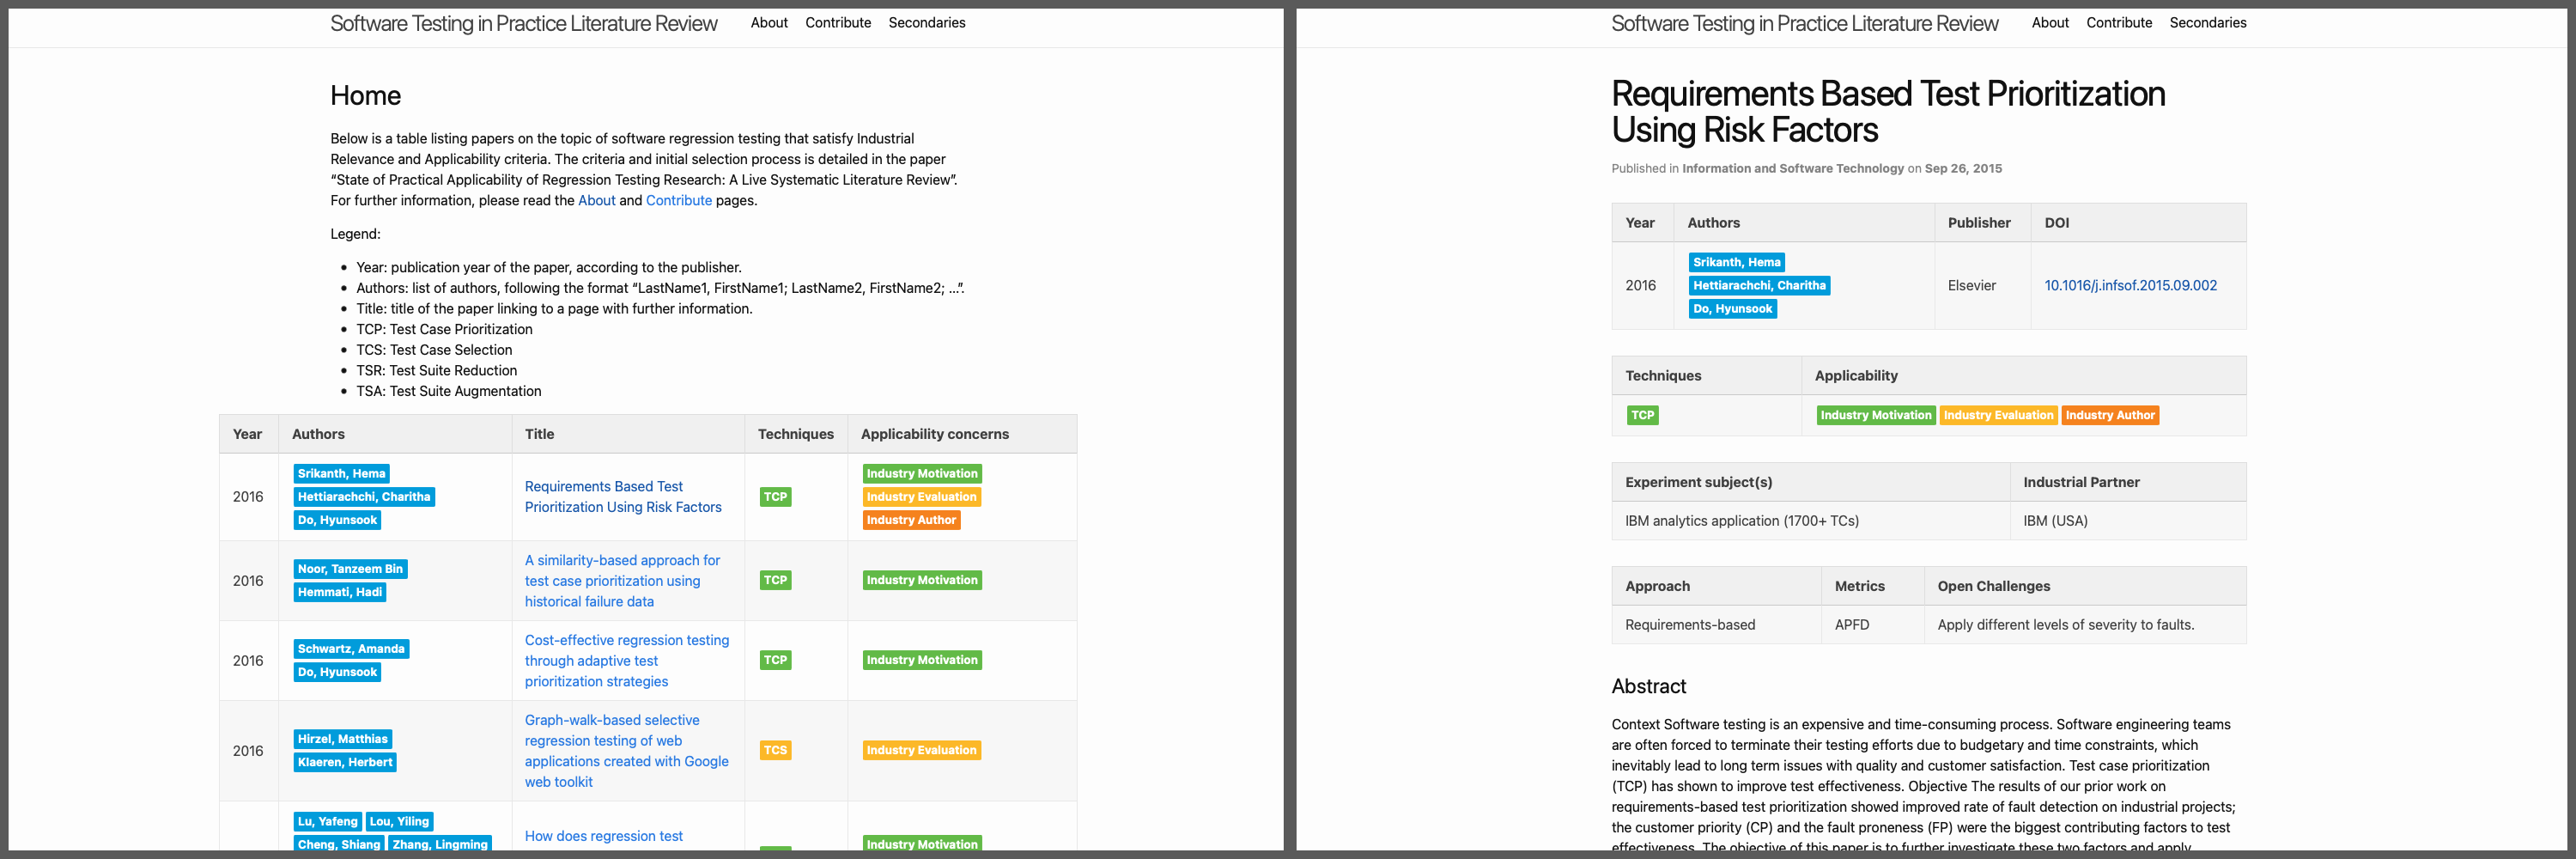
\includegraphics[width=\linewidth]{live_repository_screenshots_4.png}
%  \caption{Screenshots from the live repository. From left to right: 1) the main page listing the included papers; and 2) a single paper's page (\citetalias{srikanth_requirements_2016} used as example). }
%  \label{fig:live_repository}
%\end{figure}
%----------------------------------------------------------------------------------------
%	Conclusion
%----------------------------------------------------------------------------------------
\chapter{Conclusion}\label{chap:conclusion}
\lhead{\emph{\nameref{chap:conclusion}}}

\section{Threats to Validity}\label{sec:threats}

\subsection{Threats to \Cref{chap:literature_review} }

\paragraph{Construct validity} Despite our efforts to comprehensively find all primary studies that meet our selection criteria, we might have missed some.
To mitigate this threat, we performed a systematic search over five broad digital libraries and complemented the search with a snowballing cycle and a check with authors of all found studies, who in fact suggested a few additional entries.

As usual for this kind of study, our selection of papers was performed through queries, followed by manual filtering.
To diminish potential bias of the latter step, the filtering process was systematically reviewed and agreed upon among all the three authors.

\paragraph{Internal validity} The internal validity of this study is strongly dependent on the three research questions that guided all our analysis as well as the data extraction form we  built.
We took great care in ensuring that they properly reflect our objectives, although it is unavoidable that, by formulating  different questions or using other data extraction forms, we could have obtained other results.
We might also have overlooked or misinterpreted some important information or arguments in the primary studies, beyond our best efforts and accuracy in the full reading of all selected papers.
To mitigate such threats we provide all extracted data in traceable format, highlighting the main points we extracted from each primary study.
Furthermore, the responses we received directly from authors often provide additional context that reduce the risk of misinterpretation.
That said, we cannot make the full responses available due to non-disclosure requests from some authors.

\paragraph{Conclusion validity}
The conclusions we drew in terms of  the information  we summarize from the primary studies, the detected challenges we discuss in the above section and the recommendations we formulate in the conclusions might have been influenced by our background, and other authors might have reached different conclusions.
Such potential bias is unavoidable in this type of study, however we tried to mitigate it by aiming at full consensus of all authors behind each conclusion.
Furthermore, by documenting in detail the data extraction process, we ensure a fully transparent study that can be verified and replicated.
The survey sent to practitioners helps to validate our conclusions.
Although the sample of 23 responses is very small, it shows a degree of alignment among people working in six different countries.
A convenience sample was used to distribute the survey; thus, the practitioners we reached are more likely to have some contact with ongoing research.
To avoid excessive bias in that direction, we did not contact members of industry who are known to regularly publish in Software Engineering events.

\paragraph{External validity}
We do not make any claim of validity of our conclusions beyond the \numpapers papers analyzed.
As more primary studies are published, they should be read and analyzed on their own, and our conclusions should be revised accordingly. In consideration of this threat, in the aim of ensuring validity even in future, we are committed to keep the live repository up-to-date, taking into account the community inputs.
Moreover, we believe that the framework we developed consisting of the three research questions, the data extraction form and the structured tables for summarizing the approaches and the metrics could be still applicable also by other external authors.

\subsection{Threats to \Cref{chap:orchestration} }

We evaluated \fz using faults available in \dfj.  Our results and
conclusions could be different had we used another bug repository.
However, \dfj is among the most popular bug repositories and is
heavily used in research on regression testing.  Additionally, it
includes real faults, which strengthens our findings.

The fact that we use \dfj means that we were running experiments on
project versions that are potentially very far apart (e.g., years).
In this setup, \ek might select a very large number of tests, because
it was designed for small code changes between two
consecutive commits~\cite{gligoricEk, VasicETAL17EkstaziSharp}.  However, 
\ek ended up performing well
even in our setup.

We defined the testing budget as the number of tests that one can run
at each project version, which does not take into account the
differences in individual test execution time.  As we focus on unit
tests, we do not expect that there would be substantial differences in
execution time across tests.

To measure effectiveness, we used \ttff and \apfd. As known the \dfj subjects contain only one fault per version and hence the two measures behave similarly. 
To mitigate this issue, we need to perform more studies on subjects containing multiple faults, for which the \apfd measure becomes more valuable. 

In our experiments we assume that test execution is deterministic,
which we know  does not always hold in practice, i.e.,
tests are flaky~\cite{luo2014empirical,harman2018start}.  We have not observed any flaky behavior in our
experiments: only the expected set of tests was failing in each run.

\subsection{Threats to \Cref{chap:industry} }

These observations relate to a few teams at the company and might not generalize to software industry as a whole.

\subsection{Threats to \Cref{chap:gap} }

\section{Contributions}

The following papers produced and published during performed during this thesis.

\nociteP{rossi2020defensive_p}

\nociteP{greca_comparing_2022_p}

%\bibentry{greca_comparing_2022}
%
\nociteP{greca_live_2022_p}

\section{Conclusion}

%\input{chapters/intro}
%
%\input{chapters/background}
%
%\input{chapters/sota}
%
%\input{chapters/proposal}

%----------------------------------------------------------------------------------------
%	THESIS CONTENT - APPENDICES
%----------------------------------------------------------------------------------------

\addtocontents{toc}{\vspace{2em}} % Add a gap in the Contents, for aesthetics
%
\appendix % Cue to tell LaTeX that the following 'chapters' are Appendices

%% Include the appendices of the thesis as separate files from the Appendices folder
%% Uncomment the lines as you write the Appendices

%\lhead{\emph{Appendix A}} % Set the left side page header to "Appendix A"
%%----------------------------------------------------------------------------------------
%	Appendix A
%----------------------------------------------------------------------------------------
\chapter{Tables}\label{app:tables}
\lhead{\emph{Appendix \ref{app:tables}: \nameref{app:tables}}}

\todo{Write your Appendix content here, if needed.}
%----------------------------------------------------------------------------------------
%	Appendix B
%----------------------------------------------------------------------------------------
\chapter{Surveys}\label{app:surveys}
\lhead{\emph{Appendix \ref{app:surveys}: \nameref{app:surveys}}}

%\todo{Write your Appendix content here, if needed.}

\section{E-mail Template Sent to Authors of Surveyed Papers}
\label{sec:app_email}

\begin{tcolorbox}
\small
Dear \{\{Name\}\},

I am Renan Greca, a PhD student at the Gran Sasso Science Institute, under the supervision of Professors Antonia Bertolino and Breno Miranda. Currently, we are performing a systematic literature review on the topic of software regression testing, focusing on the real-world relevance and applicability of techniques proposed in academia.

The following paper(s) of your authorship has(have) been selected for our study:

\{\{Paper 1\}\}\\
\{\{Paper 2\}\}\\
\{\{Paper 3\}\}\\

If possible, we would like some information about the outcome of your research after the publication of the paper(s). We have a few questions regarding your work:

\textbf{1. Is there a functional version of your technique (tool, prototype, source code, etc.) available online? If so, please share with us the URL.}

\textbf{2. Was there an attempt to implement your technique in industrial or large open-source software? Is the technique currently in use with the software?}

\textbf{3. If the technique was put into practice, were the metrics used in the paper relevant for the technique’s applicability? If not, were there other metrics that proved to be useful?}

Furthermore, please let us know whether we can link your comments directly to your work in our literature review or, if not, if we can mention these comments without referencing which author gave them.

Finally, please inform us if you are interested and available for further contact related to the outcome of this research at a later date.

We kindly ask you to provide answers by September 23, or to let us know by then if more time is needed.

If you have received a similar email before, it is because we are updating our study and we have included another paper from your authorship, so please respond regarding these new paper(s).

Best regards,

Renan Greca (GSSI)\\
Breno Miranda (UFPE)\\
Antonia Bertolino (ISTI-CNR)\\
\end{tcolorbox}

\section{Questionnaire Sent to Practitioners During Literature Review}
\label{sec:app_prac_questionnaire}

\begin{table}[h!]
\centering
\small
\rowcolors{1}{}{gray!10}
%\setlength{\tabcolsep}{6pt}
\begin{tabular}{p{0.05\linewidth}p{0.9\linewidth}}
\toprule
\textbf{Nº} & \textbf{Question} \\
\midrule
\textbf{1} & \textbf{Survey for software testing practitioners}

We are researchers studying the state of collaboration between academic researchers and industrial practitioners, considering the topic of software regression testing. This survey has the goal of better understanding practitioners' perspective on past and ongoing usage of methods, techniques and tools initially developed in an academic context.

Fill this form if you are directly or indirectly involved with software testing at the company you work for. If you have colleagues that also work with software testing, please share the form with them.

Please submit your responses by {{deadline}}.

By answering these questions, you provide consent to the authors to handle this data and use it for research purposes. The data will not be used for any other purposes.

If you have questions or need clarifications, feel free to contact the authors:
Antonia Bertolino (antonia.bertolino@isti.cnr.it)
Breno Miranda (bafm@ufpe.br)
Renan Greca (renan.greca@gssi.it) \\

\textbf{1.1} & \textbf{Please tell us what are the most common pain points when it comes to running regression testing suites.}

\textit{Multiple choices can be selected.}

a) Detecting failures

b) Flaky (unreliable) tests 

c) Running time of the test suite

d) Creating new tests or updating existing ones

e) Cleaning up obsolete tests 

Other... \\

\textbf{1.2} & \textbf{Do you know of, or have you used, any tool for improving regression testing with roots in academic research?}

By regression testing, we mean running and re-running tests that cover previously-existing functionality. Examples of techniques that can help are test case selection, test case prioritization, test suite augmentation or test suite reduction.

\textit{A single choice can be selected.}

a) I have used one or more tools. (go to Section 2)

b) I know about one or more, but never used them. (go to Section 3)

c) I don't know about these tools. (go to Section 4) \\
\bottomrule
\end{tabular}\\
\caption{Questionnaire for practitioners, Section 1.}
\label{table:interview_questions}
\end{table}


\begin{table}[]
\centering
\small
\rowcolors{1}{}{gray!10}
%\setlength{\tabcolsep}{6pt}
\begin{tabular}{p{0.05\linewidth}p{0.9\linewidth}}
\toprule
\textbf{Nº} & \textbf{Question} \\
\midrule
\textbf{2} & \textbf{About the tools you have used.} 

In the previous page, you answered that you have used tools to improve regression testing. Please tell us about them.	\\

\textbf{2.1} & \textbf{Which tools have you used?}

\textit{Full body answer.}\\

\textbf{2.2} & \textbf{Please mark how much you agree with the following statements.}

If you have used multiple tools, you may offer general sentiments about them collectively.

\textit{Possible values: Strongly disagree, Disagree, Neutral, Agree, Strongly agree.}

You had a positive experience using the tool.

The tool was easy to learn and use.

The tool satisfied what you were looking for.

The tool was designed targeting your company.

The tool is currently still in use by you or your colleagues. \\

\textbf{2.3} & \textbf{Feel free to share further thoughts about your experience with the tool(s).}

\textit{Full body answer.}\\
\bottomrule
\end{tabular}\\
\caption{Questionnaire for practitioners, Section 2.}
\label{table:interview_questions}
\end{table}


\begin{table}[]
\centering
\small
\rowcolors{1}{}{gray!10}
%\setlength{\tabcolsep}{6pt}
\begin{tabular}{p{0.05\linewidth}p{0.9\linewidth}}
\toprule
\textbf{Nº} & \textbf{Question} \\
\midrule
\textbf{3} & \textbf{About the tools you know.}

In the previous page, you answered that you know about tools to improve regression testing. Please tell us which ones.	\\

\textbf{3.1} & \textbf{Which tools do you know about?}

\textit{Full body answer.}\\
\bottomrule
\end{tabular}\\
\caption{Questionnaire for practitioners, Section 3.}
\label{table:interview_questions}
\end{table}

\begin{table}[]
\centering
\small
\rowcolors{1}{}{gray!10}
%\setlength{\tabcolsep}{6pt}
\begin{tabular}{p{0.05\linewidth}p{0.9\linewidth}}
\toprule
\textbf{Nº} & \textbf{Question} \\
\midrule
\textbf{4} & \textbf{Collaboration with academia.}

This page focuses on the possibilities of collaboration between practitioners and academics.\\

\textbf{4.1} & \textbf{Please mark how much you agree with the following statements.}

\textit{Possible values: Strongly disagree, Disagree, Neutral, Agree, Strongly agree.}

You stay informed about recent research in Software Engineering.

A piece of Software Engineering research has directly improved your workflow.

You keep contact with a friend or colleague doing research in Software Engineering.

There have been attempts of collaboration between members of your company and academia.

Your company provide open datasets or open-source software that could be used as research subjects.\\

\textbf{4.2} & \textbf{If you haven't already, what would convince you to try using a technique proposed in academia in your workflow? After trying it, what should it satisfy to become a permanent part of your process?}

\textit{Full body answer.}\\

\textbf{4.3} & \textbf{If you have materials to share, such as results of previous collaborations or open-source data provided by your company, please put links below.}

\textit{Full body answer.}\\

\textbf{4.4} & \textbf{Feel free to share any other comment you might have regarding industry-academia collaboration for regression testing.}

\textit{Full body answer.}\\

\bottomrule
\end{tabular}\\
\caption{Questionnaire for practitioners, Section 4.}
\label{table:interview_questions}
\end{table}

\begin{table}[]
\centering
\small
\rowcolors{1}{}{gray!10}
%\setlength{\tabcolsep}{6pt}
\begin{tabular}{p{0.05\linewidth}p{0.9\linewidth}}
\toprule
\textbf{Nº} & \textbf{Question} \\
\midrule
\textbf{5} & \textbf{Demographics}

This final section is optional, but would help improve the quality of our results.\\

\textbf{5.1} & \textbf{Company}

The company for which you work.

\textit{Full body answer.} \\

\textbf{5.2} & \textbf{Country}

The country where you work.

\textit{A single choice can be selected, from a list of countries.} \\

\textbf{5.3} & \textbf{Role}

What title best describes your role at the company?

a) Software Engineer

b) Software Tester

c) Product Manager

d) Test Manager

Other... \\

& \textbf{Thank you for your time!} \\

\bottomrule
\end{tabular}\\
\caption{Questionnaire for practitioners, Section 5.}
\label{table:interview_questions}
\end{table}

\clearpage

\section{Questions for Practitioners at the Industrial Partner}
\label{sec:app_ind_questions}

\begin{table}[h!]
\centering
\small
\rowcolors{1}{}{gray!10}
%\setlength{\tabcolsep}{6pt}
\begin{tabular}{p{0.05\linewidth}p{0.9\linewidth}}
\toprule
\textbf{Nº} & \textbf{Question} \\
\midrule
\textbf{1} & \textbf{Roles \& education} \\
\textbf{1.1} & What is your role at the company and what are the main ways you interact with the regression testing suite? \\
\textbf{1.2} & What is your education in testing? \\
\midrule
\textbf{2} & \textbf{Are these common issues when dealing with the test suite?} \\
\textbf{2.1} & Correctly detecting failures (avoiding slips) \\
\textbf{2.2} & Flaky (unreliable tests) \\
\textbf{2.3} & Running time of the test suite \\
\textbf{2.4} & Creating or updating tests (increasing test scope) \\
\textbf{2.5} & Cleaning up obsolete tests (reducing test scope) \\
\midrule
\textbf{3} & \textbf{Current practices} \\
\textbf{3.1} & Are you familiar with these terms? Do you use them? \\
\textbf{3.1.1} & Test Case Selection \\
\textbf{3.1.2} & Test Case Prioritization \\
\textbf{3.1.3} & Test Suite Reduction \\
\textbf{3.1.4} & Test Suite Augmentation \\
\textbf{3.2} & Does your team separate test execution into shorter, frequent runs and longer overnight runs? \\
\textbf{3.3} & Are there people in your team solely responsible for testing, or is it a job of the developer? \\
\textbf{3.4} & Do you believe the current test suite is effective in avoiding fault propagation upon delivery of an update? \\
\textbf{3.5} & How often are there failing tests from the overnight run in the morning? \\
\textbf{3.6} & How often is a test failure a sign of actual SUT error vs. poor test quality vs. environment misconfiguration? \\
\textbf{3.7} & What do you do when the same test fails many days in a row? \\
\textbf{3.8} & What is the standard procedure for dealing with potentially flaky tests? \\
\textbf{3.9} & Is there a policy in place for refactoring and/or removing aging tests? \\
\textbf{3.10} & Do you have an idea of how much money or how much electricity is needed to run a test suite? Is this concern increasing or reducing over the years? \\
\textbf{3.11} & Do you personally ever review test code? How much trust do you have that it's being done correctly and at high quality? \\
\midrule
\textbf{4} & \textbf{Interaction with academia} \\
\textbf{4.1} & Do you stay informed about recent research in Software Engineering? \\
\textbf{4.2} & Has a piece of Software Engineering research directly improved your workflow? \\
\textbf{4.3} & Do you keep contact with a friend or colleague doing research in Software Engineering? \\
\textbf{4.4} & Before me, have there been attempts of collaboration between members of your team and academic researchers? \\
\textbf{4.5} & What does a tool need to do/have in order to convince you to use it as a permanent part of your workflow? \\
\textbf{4.6} & What are the risks and benefits of using a new tool for regression testing improvement? \\
\textbf{4.7} & Have you ever used an open-source regression testing approach as-is, or is it always necessary to re-engineer it for usability/security/compatibility reasons? \\
\textbf{4.8} & If I came to you saying ``I have this algorithm that would help your testing workflow'', what would be your reaction? \\
\bottomrule
\end{tabular}\\
\caption{List of questions asked during interviews.}
\label{table:interview_questions}
\end{table}

\addtocontents{toc}{\vspace{2em}} % Add a gap in the Contents, for aesthetics

\backmatter

\clearpage

%----------------------------------------------------------------------------------------
%	BIBLIOGRAPHY
%----------------------------------------------------------------------------------------

\label{Bibliography}

%\newcites{P}{Papers related to this thesis}
%\newcites{C}{Conferences related to this thesis}

%\fullcite{greca_comparing_2022}

%\bibliographystylec{IEEEtran}
%
%\nocitec{greca_comparing_2022}

%\bibliography{bibliographies/production.bib}

%\printbibliography

\lhead{\emph{Bibliography}} % Change the page header to say "Bibliography"

%\bibliographystyleP{unsrtnat}
%\bibliographyP{production.bib}

%\bibliographystyleS{unsrtnat}
%\bibliographyS{slr.bib}

%\nociteS{srikanth_requirements_2016}
\nociteS{noor_similarity-based_2016}
\nociteS{schwartz_cost-effective_2016}
\nociteS{hirzel_graph-walk-based_2016}
\nociteS{lu_how_2016}
\nociteS{vost_trace-based_2016}
\nociteS{wang_enhancing_2016}
\nociteS{srikanth_test_2016}
\nociteS{blondeau_test_2017}
\nociteS{pradhan_search-based_2016}
\nociteS{buchgeher_improving_2016}
\nociteS{tahvili_dynamic_2016}
\nociteS{oqvist_extraction-based_2016}
\nociteS{magalhaes_automatic_2016}
\nociteS{aman_application_2016}
\nociteS{busjaeger_learning_2016}
\nociteS{yoshida_fsx_2016}
\nociteS{tahvili_cost-benefit_2016}
\nociteS{ramler_tool_2017}
\nociteS{strandberg_experience_2016}
\nociteS{marijan_effect_2016}
\nociteS{gotlieb_using_2017}
\nociteS{chi_multi-level_2017}
\nociteS{bach_coverage-based_2017}
\nociteS{spieker_reinforcement_2017}
\nociteS{vasic_file-level_2017}
\nociteS{celik_regression_2017}
\nociteS{ouriques_test_2018}
\nociteS{kwon_cost-effective_2017}
\nociteS{garousi_multi-objective_2018}
\nociteS{shi_evaluating_2018}
\nociteS{haghighatkhah_test_2018}
\nociteS{zhang_hybrid_2018}
\nociteS{miranda_fast_2018}
\nociteS{yilmaz_case_2018}
\nociteS{chen_optimizing_2018}
\nociteS{celik_regression_2018}
\nociteS{zhu_test_2018}
\nociteS{azizi_retest_2018}
\nociteS{guo_decomposing_2019}
\nociteS{zhong_testsage:_2019}
\nociteS{fu_resurgence_2019}
\nociteS{eda_efficient_2019}
\nociteS{goyal_test_2019}
\nociteS{yu_terminator_2019}
\nociteS{correia_motsd_2019}
\nociteS{machalica_predictive_2018}
\nociteS{najafi_improving_2019}
\nociteS{leong_assessing_2019}
\nociteS{cruciani_scalable_2019}
\nociteS{philip_fastlane:_2019}
\nociteS{magalhaes_hsp_2020}
\nociteS{wu_time_2019}
\nociteS{land_industrial_2019}
\nociteS{noemmer_evaluation_2020}
\nociteS{lubke_selecting_2020}
\nociteS{yackley_simultaneous_2019}
\nociteS{shi_understanding_2019}
\nociteS{lima_multi-armed_2022}
\nociteS{zhou_beating_2020}
\nociteS{peng_empirically_2020}
\nociteS{bertolino_learning--rank_2020}
\nociteS{chen_multi-objective_2021}
\nociteS{zarges_artificial_2021}
\nociteS{bagherzadeh_reinforcement_2022}
\nociteS{elsner_empirically_2021}
\nociteS{pan_dynamic_2020}
\nociteS{mehta_data-driven_2021}
\nociteS{xu_requirement-based_2021}
\nociteS{zhou_parallel_2022}
\nociteS{sharif_deeporder_2021}
\nociteS{li_aga_2021}
\nociteS{chen_context-aware_2021}
\nociteS{zhang_comparing_2022}
\nociteS{abdelkarim_tcp-net_2022}
\nociteS{cingil_black-box_2022}
\nociteS{yaraghi_scalable_2022}
\nociteS{omri_learning_2022}
\nociteS{greca_comparing_2022}


%\begin{refsection}[S]
%    \printbibliography[heading=S]
%\end{refsection}

%\begin{refsection}[S]
%	\newrefcontext[labelprefix=S]
%%	\nocite{*}
%    \printbibliography[heading=S]
%\end{refsection}

\newrefcontext[sorting=nyt]
\printbibliography
%\bibliographystyle{unsrtnat} % Use the "unsrtnat" BibTeX style for formatting the Bibliography
%\bibliography{secondaries.bib,bibliography.bib,production.bib,slr.bib} % This contains only the 
%\bibliography{}

\end{document}